\documentclass[12pt,a4paper,twoside,openright]{report}
%
%-----Packages
%
\usepackage[english]{babel}
\usepackage{setspace}
\usepackage[T1]{fontenc}
\usepackage[latin1]{inputenc}
\usepackage[intlimits]{amsmath}
\usepackage{amsfonts,amssymb}
\usepackage{natbib}
\usepackage[normalsize,bf]{caption}
\usepackage[dvips]{graphicx}
\usepackage{color}
\usepackage[breaklinks,linktocpage]{hyperref}
\usepackage{fancyhdr}
\usepackage{setspace}
\usepackage{subfigure}
\usepackage{float}
\usepackage{lettrine}
\usepackage{comment}
\usepackage{pifont}
\usepackage{soul, color}  %\hl
\usepackage{booktabs}	  %\toprule in table
\usepackage{tabularx}	  %\tabular
\usepackage{multicol}	  %table col
\usepackage{multirow}	  %table row
\usepackage{diagbox}

\newcommand{\hlg}[2][green]{{\sethlcolor{#1}\hl{#2}}}
\newcommand{\tabincell}[2]{\begin{tabular}{@{}#1@{}}#2\end{tabular}}
\sloppy\par
%****************************************************************
% ===========Optional packages (uncomment as needed)=============
%****************************************************************
\usepackage{wrapfig}
%\usepackage{makeidx}
\usepackage{amsbsy}
\usepackage{latexsym}
\usepackage{amsthm}
\usepackage{datatool}
%\usepackage{glossary}
\usepackage{glossaries}
%\makeglossary
%\makeglossaries


%=======================================================
%
%-----Layout
%
\onehalfspacing
\hoffset = -1 in
\voffset= -1 in
%
%-----Set margins for a4 paper
%
\topmargin = 3.0cm
\textwidth = 17cm
\textheight = 22cm
\oddsidemargin =  2cm
\evensidemargin = 2cm
%
%-----Headers and Footers
%
\pagestyle{fancyplain}
\renewcommand{\chaptermark}[1]%
{\markboth{#1}{}}
\renewcommand{\sectionmark}[1]%
{\markright{\thesection\ -- #1}}
\lhead[\fancyplain{}{\thepage}]%
{\fancyplain{}{\rightmark}}
\rhead[\fancyplain{}{\leftmark}]%
{\fancyplain{}{\thepage}}
\cfoot{}
%
%-----No headers on empty pages before new chapter
%
\makeatletter
\def\cleardoublepage{\clearpage\if@twoside \ifodd\c@page\else
	\hbox{}
	\thispagestyle{plain}
	\newpage
	\if@twocolumn\hbox{}\newpage\fi\fi\fi}
\makeatother \clearpage{\pagestyle{plain}\cleardoublepage}
%
%-----Footnotes
%
\renewcommand{\thefootnote}{\fnsymbol{footnote}} % Footnotes are marked with symbols instead of literals
\setlength{\textfloatsep}{8pt plus 4pt minus 4pt}        % Separation of floats from text
\renewcommand{\bibnumfmt}[1]{{\scriptsize #1}}
\setlength{\bibhang}{2em}
%
%-----Define Horizontal rule
%
\newcommand{\HRule}{\rule{\textwidth}{0.5mm}}
%
%-----Define Hyperlink colors
%
\definecolor{darkred}{rgb}{0.25,0,0}
\definecolor{darkgreen}{rgb}{0,0.25,0}
\definecolor{darkblue}{rgb}{0,0,0.5}
\hypersetup{colorlinks,linkcolor=black,filecolor=black,urlcolor=darkblue,citecolor=black}
\usepackage{breakurl}
%****************************************************************
% ===========Add user definitions as needed=====================
%****************************************************************
%\include{definitions}
\newtheorem{theorem}{Theorem}[chapter]
\newtheorem{principle}{Principle}[chapter]
\newtheorem{algorithm}{Algorithm}[chapter]
\newtheorem{law}{Law}
%\theoremstyle{plain}  % Default
\theoremstyle{definition}
%\theoremstyle{remark}
\newtheorem{problem}{Problem}[chapter]
\newtheorem{example}{Example}[chapter]
\newtheorem{definition}{Definition}[chapter]




%%***********Config file orginal backup*********
%\immediate\write18{makeindex \jobname.nlo -s nomencl.ist -o \jobname.nls}
%\documentclass[12pt,a4paper,twoside,openright]{report}
%%
%%-----Packages
%%
%\usepackage[english]{babel}
%\usepackage{setspace}
%\usepackage[T1]{fontenc}
%\usepackage[latin1]{inputenc}
%\usepackage[intlimits]{amsmath}
%\usepackage{amsfonts,amssymb}
%\usepackage{natbib}
%\usepackage[normalsize,bf]{caption}
%\usepackage[dvips]{graphicx}
%%\usepackage{color}
%%\usepackage{mathdots}
%%\usepackage{mathtools}
%%\usepackage{booktabs}
%%\usepackage{multirow}
%%\usepackage{ps2pdf}
%\usepackage{epstopdf}
%\usepackage[breaklinks,linktocpage]{hyperref}
%\usepackage{fancyhdr}
%\usepackage{setspace}
%\usepackage{subfigure}
%\usepackage{lettrine}
%\newcommand{\tabincell}[2]{\begin{tabular}{@{}#1@{}}#2\end{tabular}}
%\sloppy\par
%%****************************************************************
%% ===========Optional packages (uncomment as needed)=============
%%****************************************************************
%\usepackage{wrapfig}
%%\usepackage{makeidx}
%\usepackage{amsbsy}
%\usepackage{latexsym}
%\usepackage{amsthm}
%\usepackage{datatool}
%\usepackage{nomencl}
%\makenomenclature
%\usepackage{glossaries}
%\makeglossaries
%\usepackage{ifthen}
%\usepackage{graphicx}
%\usepackage{color, soul}
%%\usepackage{wasysym}
%%\usepackage{psfrag}
%%\usepackage{subfig}
%%\usepackage{pifont}
%%\usepackage{longtable}
%%\setlength\LTleft{0pt}
%%\setlength\LTright{0pt}
%%=======================================================
%%
%%-----Layout
%%
%\onehalfspacing
%\hoffset = -1 in
%\voffset= -1 in
%%
%%-----Set margins for a4 paper
%%
%\topmargin = 3.0cm
%\textwidth = 17cm
%\textheight = 22cm
%\oddsidemargin =  2cm
%\evensidemargin = 2cm
%%
%%-----Headers and Footers
%%
%\pagestyle{fancyplain}
%\renewcommand{\chaptermark}[1]%
%            {\markboth{#1}{}}
%\renewcommand{\sectionmark}[1]%
%            {\markright{\thesection\ -- #1}}
%\lhead[\fancyplain{}{\thepage}]%
%      {\fancyplain{}{\rightmark}}
%\rhead[\fancyplain{}{\leftmark}]%
%     {\fancyplain{}{\thepage}}
%\cfoot{}
%%
%%-----No headers on empty pages before new chapter
%%
%\makeatletter
%\def\cleardoublepage{\clearpage\if@twoside \ifodd\c@page\else
%    \hbox{}
%    \thispagestyle{plain}
%    \newpage
%    \if@twocolumn\hbox{}\newpage\fi\fi\fi}
%\makeatother \clearpage{\pagestyle{plain}\cleardoublepage}
%%
%%-----Footnotes
%%
%\renewcommand{\thefootnote}{\fnsymbol{footnote}} % Footnotes are marked with symbols instead of literals
%\setlength{\textfloatsep}{8pt plus 4pt minus 4pt}        % Separation of floats from text
%\renewcommand{\bibnumfmt}[1]{{\scriptsize #1}}
%\setlength{\bibhang}{2em}
%%
%%-----Define Horizontal rule
%%
%\newcommand{\HRule}{\rule{\textwidth}{0.5mm}}
%%
%%-----Define Hyperlink colors
%%
%\definecolor{darkred}{rgb}{0.25,0,0}
%\definecolor{darkgreen}{rgb}{0,0.25,0}
%\definecolor{darkblue}{rgb}{0,0,0.5}
%\hypersetup{colorlinks,linkcolor=black,filecolor=black,urlcolor=darkblue,citecolor=black}
%\usepackage{breakurl}
%
%%****************************************************************
%% ===========Add user definitions as needed=====================
%%****************************************************************
%\include{definitions}
%\newtheorem{theorem}{Theorem}[chapter]
%\newtheorem{principle}{Principle}[chapter]
%%\newtheorem{algorithm}{Algorithm}[chapter]
%\newtheorem{law}{Law}
%%\theoremstyle{plain}  % Default
%\theoremstyle{definition}
%%\theoremstyle{remark}
%\newtheorem{problem}{Problem}[chapter]
%\newtheorem{example}{Example}[chapter]
%\newtheorem{definition}{Definition}[chapter]
%%=======================================================
%%%%%%%%%%%%%
%%-----Begin Document
%%%%%%%%%%%%%
%\begin{document}
%\pagenumbering{roman}
%%
%%-----Title page
%%
%
%\begin{titlepage}
%\noindent {\bf Shanghai Jiao Tong University \\
%University of Michigan- Shanghai Jiao Tong University Joint Institute}\\
%\noindent \HRule \vspace{0.0455\textheight}
%%****************************************************************
%% ===========Edit the following lines to get the right title============
%%****************************************************************
%\begin{center}
%{\huge \bf Proposal Name}\\[0.016\textheight]
%{\Large \bf Doctoral Dissertation Proposal} \\[0.032\textheight]
%\large{by} \\[0.032\textheight] \Large{ \bf Jibin Song}\\
%%=======================================================
%\vspace{5cm}
%\normalsize{A proposal submitted in satisfaction of the \\
%requirements for the degree of Doctor of Philosophy in \\
%Control Science and Engineering at Shanghai Jiao Tong University}
%\HRule \\[0.023\textheight]
%%****************************************************************
%%======Edit the following lines to get the right committee members======
%%****************************************************************
%\begin{tabular*}{\textwidth}{@{}l@{\extracolsep{\fill}}r@{}}
%\textbf{Committee in charge:} &  \textbf{Shanghai}\\
%\textbf{Professor XXX} &  \textbf{July, 2020}\\
%\textbf{Professor XXX} & \\
%\textbf{Professor XXX} & \\
%\textbf{Professor XXX} & \\
%\textbf{Professor XXX} & \\
%\end{tabular*}
%%=======================================================
%\end{center}
%\end{titlepage}
%
%%
%%-----Abstract
%%
%\thispagestyle{empty}
%\cleardoublepage
%%****************************************************************
%%===========Your abstract goes in the file Abstract.tex==============
%%****************************************************************
%
%
%
%\begin{abstract}
\noindent

Here is the abstract. Here is the abstract. Here is the abstract. Here is the abstract.

Here is the abstract. Here is the abstract. Here is the abstract. Here is the abstract.

Here is the abstract. Here is the abstract. Here is the abstract. Here is the abstract.

Here is the abstract. Here is the abstract. Here is the abstract. Here is the abstract.

Here is the abstract. Here is the abstract. Here is the abstract. Here is the abstract.

Here is the abstract. Here is the abstract. Here is the abstract. Here is the abstract.

Here is the abstract. Here is the abstract. Here is the abstract. Here is the abstract.

Here is the abstract. Here is the abstract. Here is the abstract. Here is the abstract.
\end{abstract}



%\cleardoublepage
%\newlength{\nomitemorigsep}
\setlength{\nomitemorigsep}{\nomitemsep}
\setlength{\nomitemsep}{-\parsep}
\makenomenclature
\renewcommand{\nomgroup}[1]{%
  \itemsep\nomitemorigsep%
  \ifthenelse{%
    \equal{#1}{A}%
  }{%
  \item[\textbf{Abbreviations}]%

  }{%
    \ifthenelse{\equal{#1}{S}}{%
    \item[\textbf{List of Symbols}]%

    }{}%
  }%
  \itemsep\nomitemsep
}
\renewcommand{\nomname}{Nomenclature}
\markboth{\MakeUppercase\nomname}{\MakeUppercase\nomname}
\printnomenclature[0.8in]
\nomenclature[A]{ADS}{Advanced Design System}
\nomenclature[A]{ESR}{Equivalent series resistance}
\nomenclature[A]{MOSFET}{Metal-oxide-semiconductor field effect transistor}
\nomenclature[A]{MWPT}{Multiple-receiver wrieless power transfer}
\nomenclature[A]{PA}{Power amplifier}
\nomenclature[A]{RF}{Radio frequency}
\nomenclature[A]{SRR}{Synchronous Resonant Rectifier}
\nomenclature[A]{WPT}{Wireless power transfer}
\nomenclature[A]{ZVS}{Zero-voltage-switching}




\nomenclature[S]{$C_{0}$}{Capacitor in resonant tank of Class E PA}
\nomenclature[S]{$C_{r}$}{Diode/switch shunt capacitor of Class E rectifier}
\nomenclature[S]{$C_{S}$}{Switch shunt capacitor of Class E PA}
\nomenclature[S]{$C_{rx}$}{Compensation capacitor of receiving coil}
\nomenclature[S]{$C_{tx}$}{Compensation capacitor of transmitting coil}
\nomenclature[S]{$k$}{Mutual inductance coefficient of coupling coils}
\nomenclature[S]{$k_{ij}$}{Mutual inductance coefficient between $i$-th and $j$-th coils in MWPT}
\nomenclature[S]{$L_{0}$}{Inductor in resonant tank of Class E PA}
\nomenclature[S]{$L_{rx}$}{Inductance of receiving coil}
\nomenclature[S]{$L_{tx}$}{Inductance of transmitting coil}
\nomenclature[S]{$M$}{Mutual inductance of coupling coils}
\nomenclature[S]{$M_{ij}$}{Mutual inductance between $i$-th and $j$-th coils in MWPT}
\nomenclature[S]{$r_{rx}$}{ESR of receiving coil}
\nomenclature[S]{$r_{tx}$}{ESR of transmitting coil}
\nomenclature[S]{$R_{L}$}{Dc load of rectifier}
\nomenclature[S]{$R_{rec}$}{Input resisance of rectifier}
\nomenclature[S]{$v_{DS}$}{Drain-source voltage of MOSFET}
\nomenclature[S]{$v_{GS}$}{Gate-source voltage of MOSFET}
\nomenclature[S]{$X_{rec}$}{Input reactance of rectifier}
\nomenclature[S]{$Z_{rec}$}{Input impedance of rectifier}
\nomenclature[S]{$Z_{coil}$}{Input impedance of transmitting coil}
\nomenclature[S]{$\eta_{PA}$}{Efficiency of PA}
\nomenclature[S]{$\eta_{rec}$}{Efficiency of rectifier}
\nomenclature[S]{$\eta_{sys}$}{Dc-dc efficiency of WPT system}
\nomenclature[S]{$\eta_{coil2load}$}{Power transfer efficiency from transmitting coil to dc load}


\cleardoublepage 







%\cleardoublepage
%%\printglossary
%%=======================================================
%%
%%-----Table of contents
%%
%%\clearpage
%\setcounter{tocdepth}{1}
%\setcounter{page}{1}
%\tableofcontents
%\doublespacing
%\listoffigures
%\doublespacing
%\listoftables
%\doublespacing
%
%
%
%
%
%\setcounter{page}{1}
%\pagenumbering{arabic}
%%****************************************************************
%%================Include each chapter in a different file===========
%%======For large theses, chapters should be in different directories=======
%%=============Add \cleardoublepage between each chapter==========
%%****************************************************************
%\ifx\allfiles\undefined   
	\documentclass[12pt,a4paper,twoside,openright]{report}
%
%-----Packages
%
\usepackage[english]{babel}
\usepackage{setspace}
\usepackage[T1]{fontenc}
\usepackage[latin1]{inputenc}
\usepackage[intlimits]{amsmath}
\usepackage{amsfonts,amssymb}
\usepackage{natbib}
\usepackage[normalsize,bf]{caption}
\usepackage[dvips]{graphicx}
\usepackage{color}
\usepackage[breaklinks,linktocpage]{hyperref}
\usepackage{fancyhdr}
\usepackage{setspace}
\usepackage{subfigure}
\usepackage{float}
\usepackage{lettrine}
\usepackage{comment}
\usepackage{pifont}
\usepackage{soul, color}  %\hl
\usepackage{booktabs}	  %\toprule in table
\usepackage{tabularx}	  %\tabular
\usepackage{multicol}	  %table col
\usepackage{multirow}	  %table row
\usepackage{diagbox}

\newcommand{\hlg}[2][green]{{\sethlcolor{#1}\hl{#2}}}
\newcommand{\tabincell}[2]{\begin{tabular}{@{}#1@{}}#2\end{tabular}}
\sloppy\par
%****************************************************************
% ===========Optional packages (uncomment as needed)=============
%****************************************************************
\usepackage{wrapfig}
%\usepackage{makeidx}
\usepackage{amsbsy}
\usepackage{latexsym}
\usepackage{amsthm}
\usepackage{datatool}
%\usepackage{glossary}
\usepackage{glossaries}
%\makeglossary
%\makeglossaries


%=======================================================
%
%-----Layout
%
\onehalfspacing
\hoffset = -1 in
\voffset= -1 in
%
%-----Set margins for a4 paper
%
\topmargin = 3.0cm
\textwidth = 17cm
\textheight = 22cm
\oddsidemargin =  2cm
\evensidemargin = 2cm
%
%-----Headers and Footers
%
\pagestyle{fancyplain}
\renewcommand{\chaptermark}[1]%
{\markboth{#1}{}}
\renewcommand{\sectionmark}[1]%
{\markright{\thesection\ -- #1}}
\lhead[\fancyplain{}{\thepage}]%
{\fancyplain{}{\rightmark}}
\rhead[\fancyplain{}{\leftmark}]%
{\fancyplain{}{\thepage}}
\cfoot{}
%
%-----No headers on empty pages before new chapter
%
\makeatletter
\def\cleardoublepage{\clearpage\if@twoside \ifodd\c@page\else
	\hbox{}
	\thispagestyle{plain}
	\newpage
	\if@twocolumn\hbox{}\newpage\fi\fi\fi}
\makeatother \clearpage{\pagestyle{plain}\cleardoublepage}
%
%-----Footnotes
%
\renewcommand{\thefootnote}{\fnsymbol{footnote}} % Footnotes are marked with symbols instead of literals
\setlength{\textfloatsep}{8pt plus 4pt minus 4pt}        % Separation of floats from text
\renewcommand{\bibnumfmt}[1]{{\scriptsize #1}}
\setlength{\bibhang}{2em}
%
%-----Define Horizontal rule
%
\newcommand{\HRule}{\rule{\textwidth}{0.5mm}}
%
%-----Define Hyperlink colors
%
\definecolor{darkred}{rgb}{0.25,0,0}
\definecolor{darkgreen}{rgb}{0,0.25,0}
\definecolor{darkblue}{rgb}{0,0,0.5}
\hypersetup{colorlinks,linkcolor=black,filecolor=black,urlcolor=darkblue,citecolor=black}
\usepackage{breakurl}
%****************************************************************
% ===========Add user definitions as needed=====================
%****************************************************************
%\include{definitions}
\newtheorem{theorem}{Theorem}[chapter]
\newtheorem{principle}{Principle}[chapter]
\newtheorem{algorithm}{Algorithm}[chapter]
\newtheorem{law}{Law}
%\theoremstyle{plain}  % Default
\theoremstyle{definition}
%\theoremstyle{remark}
\newtheorem{problem}{Problem}[chapter]
\newtheorem{example}{Example}[chapter]
\newtheorem{definition}{Definition}[chapter]




%%***********Config file orginal backup*********
%\immediate\write18{makeindex \jobname.nlo -s nomencl.ist -o \jobname.nls}
%\documentclass[12pt,a4paper,twoside,openright]{report}
%%
%%-----Packages
%%
%\usepackage[english]{babel}
%\usepackage{setspace}
%\usepackage[T1]{fontenc}
%\usepackage[latin1]{inputenc}
%\usepackage[intlimits]{amsmath}
%\usepackage{amsfonts,amssymb}
%\usepackage{natbib}
%\usepackage[normalsize,bf]{caption}
%\usepackage[dvips]{graphicx}
%%\usepackage{color}
%%\usepackage{mathdots}
%%\usepackage{mathtools}
%%\usepackage{booktabs}
%%\usepackage{multirow}
%%\usepackage{ps2pdf}
%\usepackage{epstopdf}
%\usepackage[breaklinks,linktocpage]{hyperref}
%\usepackage{fancyhdr}
%\usepackage{setspace}
%\usepackage{subfigure}
%\usepackage{lettrine}
%\newcommand{\tabincell}[2]{\begin{tabular}{@{}#1@{}}#2\end{tabular}}
%\sloppy\par
%%****************************************************************
%% ===========Optional packages (uncomment as needed)=============
%%****************************************************************
%\usepackage{wrapfig}
%%\usepackage{makeidx}
%\usepackage{amsbsy}
%\usepackage{latexsym}
%\usepackage{amsthm}
%\usepackage{datatool}
%\usepackage{nomencl}
%\makenomenclature
%\usepackage{glossaries}
%\makeglossaries
%\usepackage{ifthen}
%\usepackage{graphicx}
%\usepackage{color, soul}
%%\usepackage{wasysym}
%%\usepackage{psfrag}
%%\usepackage{subfig}
%%\usepackage{pifont}
%%\usepackage{longtable}
%%\setlength\LTleft{0pt}
%%\setlength\LTright{0pt}
%%=======================================================
%%
%%-----Layout
%%
%\onehalfspacing
%\hoffset = -1 in
%\voffset= -1 in
%%
%%-----Set margins for a4 paper
%%
%\topmargin = 3.0cm
%\textwidth = 17cm
%\textheight = 22cm
%\oddsidemargin =  2cm
%\evensidemargin = 2cm
%%
%%-----Headers and Footers
%%
%\pagestyle{fancyplain}
%\renewcommand{\chaptermark}[1]%
%            {\markboth{#1}{}}
%\renewcommand{\sectionmark}[1]%
%            {\markright{\thesection\ -- #1}}
%\lhead[\fancyplain{}{\thepage}]%
%      {\fancyplain{}{\rightmark}}
%\rhead[\fancyplain{}{\leftmark}]%
%     {\fancyplain{}{\thepage}}
%\cfoot{}
%%
%%-----No headers on empty pages before new chapter
%%
%\makeatletter
%\def\cleardoublepage{\clearpage\if@twoside \ifodd\c@page\else
%    \hbox{}
%    \thispagestyle{plain}
%    \newpage
%    \if@twocolumn\hbox{}\newpage\fi\fi\fi}
%\makeatother \clearpage{\pagestyle{plain}\cleardoublepage}
%%
%%-----Footnotes
%%
%\renewcommand{\thefootnote}{\fnsymbol{footnote}} % Footnotes are marked with symbols instead of literals
%\setlength{\textfloatsep}{8pt plus 4pt minus 4pt}        % Separation of floats from text
%\renewcommand{\bibnumfmt}[1]{{\scriptsize #1}}
%\setlength{\bibhang}{2em}
%%
%%-----Define Horizontal rule
%%
%\newcommand{\HRule}{\rule{\textwidth}{0.5mm}}
%%
%%-----Define Hyperlink colors
%%
%\definecolor{darkred}{rgb}{0.25,0,0}
%\definecolor{darkgreen}{rgb}{0,0.25,0}
%\definecolor{darkblue}{rgb}{0,0,0.5}
%\hypersetup{colorlinks,linkcolor=black,filecolor=black,urlcolor=darkblue,citecolor=black}
%\usepackage{breakurl}
%
%%****************************************************************
%% ===========Add user definitions as needed=====================
%%****************************************************************
%\include{definitions}
%\newtheorem{theorem}{Theorem}[chapter]
%\newtheorem{principle}{Principle}[chapter]
%%\newtheorem{algorithm}{Algorithm}[chapter]
%\newtheorem{law}{Law}
%%\theoremstyle{plain}  % Default
%\theoremstyle{definition}
%%\theoremstyle{remark}
%\newtheorem{problem}{Problem}[chapter]
%\newtheorem{example}{Example}[chapter]
%\newtheorem{definition}{Definition}[chapter]
%%=======================================================
%%%%%%%%%%%%%
%%-----Begin Document
%%%%%%%%%%%%%
%\begin{document}
%\pagenumbering{roman}
%%
%%-----Title page
%%
%
%\begin{titlepage}
%\noindent {\bf Shanghai Jiao Tong University \\
%University of Michigan- Shanghai Jiao Tong University Joint Institute}\\
%\noindent \HRule \vspace{0.0455\textheight}
%%****************************************************************
%% ===========Edit the following lines to get the right title============
%%****************************************************************
%\begin{center}
%{\huge \bf Proposal Name}\\[0.016\textheight]
%{\Large \bf Doctoral Dissertation Proposal} \\[0.032\textheight]
%\large{by} \\[0.032\textheight] \Large{ \bf Jibin Song}\\
%%=======================================================
%\vspace{5cm}
%\normalsize{A proposal submitted in satisfaction of the \\
%requirements for the degree of Doctor of Philosophy in \\
%Control Science and Engineering at Shanghai Jiao Tong University}
%\HRule \\[0.023\textheight]
%%****************************************************************
%%======Edit the following lines to get the right committee members======
%%****************************************************************
%\begin{tabular*}{\textwidth}{@{}l@{\extracolsep{\fill}}r@{}}
%\textbf{Committee in charge:} &  \textbf{Shanghai}\\
%\textbf{Professor XXX} &  \textbf{July, 2020}\\
%\textbf{Professor XXX} & \\
%\textbf{Professor XXX} & \\
%\textbf{Professor XXX} & \\
%\textbf{Professor XXX} & \\
%\end{tabular*}
%%=======================================================
%\end{center}
%\end{titlepage}
%
%%
%%-----Abstract
%%
%\thispagestyle{empty}
%\cleardoublepage
%%****************************************************************
%%===========Your abstract goes in the file Abstract.tex==============
%%****************************************************************
%
%
%
%\begin{abstract}
\noindent

Here is the abstract. Here is the abstract. Here is the abstract. Here is the abstract.

Here is the abstract. Here is the abstract. Here is the abstract. Here is the abstract.

Here is the abstract. Here is the abstract. Here is the abstract. Here is the abstract.

Here is the abstract. Here is the abstract. Here is the abstract. Here is the abstract.

Here is the abstract. Here is the abstract. Here is the abstract. Here is the abstract.

Here is the abstract. Here is the abstract. Here is the abstract. Here is the abstract.

Here is the abstract. Here is the abstract. Here is the abstract. Here is the abstract.

Here is the abstract. Here is the abstract. Here is the abstract. Here is the abstract.
\end{abstract}



%\cleardoublepage
%\newlength{\nomitemorigsep}
\setlength{\nomitemorigsep}{\nomitemsep}
\setlength{\nomitemsep}{-\parsep}
\makenomenclature
\renewcommand{\nomgroup}[1]{%
  \itemsep\nomitemorigsep%
  \ifthenelse{%
    \equal{#1}{A}%
  }{%
  \item[\textbf{Abbreviations}]%

  }{%
    \ifthenelse{\equal{#1}{S}}{%
    \item[\textbf{List of Symbols}]%

    }{}%
  }%
  \itemsep\nomitemsep
}
\renewcommand{\nomname}{Nomenclature}
\markboth{\MakeUppercase\nomname}{\MakeUppercase\nomname}
\printnomenclature[0.8in]
\nomenclature[A]{ADS}{Advanced Design System}
\nomenclature[A]{ESR}{Equivalent series resistance}
\nomenclature[A]{MOSFET}{Metal-oxide-semiconductor field effect transistor}
\nomenclature[A]{MWPT}{Multiple-receiver wrieless power transfer}
\nomenclature[A]{PA}{Power amplifier}
\nomenclature[A]{RF}{Radio frequency}
\nomenclature[A]{SRR}{Synchronous Resonant Rectifier}
\nomenclature[A]{WPT}{Wireless power transfer}
\nomenclature[A]{ZVS}{Zero-voltage-switching}




\nomenclature[S]{$C_{0}$}{Capacitor in resonant tank of Class E PA}
\nomenclature[S]{$C_{r}$}{Diode/switch shunt capacitor of Class E rectifier}
\nomenclature[S]{$C_{S}$}{Switch shunt capacitor of Class E PA}
\nomenclature[S]{$C_{rx}$}{Compensation capacitor of receiving coil}
\nomenclature[S]{$C_{tx}$}{Compensation capacitor of transmitting coil}
\nomenclature[S]{$k$}{Mutual inductance coefficient of coupling coils}
\nomenclature[S]{$k_{ij}$}{Mutual inductance coefficient between $i$-th and $j$-th coils in MWPT}
\nomenclature[S]{$L_{0}$}{Inductor in resonant tank of Class E PA}
\nomenclature[S]{$L_{rx}$}{Inductance of receiving coil}
\nomenclature[S]{$L_{tx}$}{Inductance of transmitting coil}
\nomenclature[S]{$M$}{Mutual inductance of coupling coils}
\nomenclature[S]{$M_{ij}$}{Mutual inductance between $i$-th and $j$-th coils in MWPT}
\nomenclature[S]{$r_{rx}$}{ESR of receiving coil}
\nomenclature[S]{$r_{tx}$}{ESR of transmitting coil}
\nomenclature[S]{$R_{L}$}{Dc load of rectifier}
\nomenclature[S]{$R_{rec}$}{Input resisance of rectifier}
\nomenclature[S]{$v_{DS}$}{Drain-source voltage of MOSFET}
\nomenclature[S]{$v_{GS}$}{Gate-source voltage of MOSFET}
\nomenclature[S]{$X_{rec}$}{Input reactance of rectifier}
\nomenclature[S]{$Z_{rec}$}{Input impedance of rectifier}
\nomenclature[S]{$Z_{coil}$}{Input impedance of transmitting coil}
\nomenclature[S]{$\eta_{PA}$}{Efficiency of PA}
\nomenclature[S]{$\eta_{rec}$}{Efficiency of rectifier}
\nomenclature[S]{$\eta_{sys}$}{Dc-dc efficiency of WPT system}
\nomenclature[S]{$\eta_{coil2load}$}{Power transfer efficiency from transmitting coil to dc load}


\cleardoublepage 







%\cleardoublepage
%%\printglossary
%%=======================================================
%%
%%-----Table of contents
%%
%%\clearpage
%\setcounter{tocdepth}{1}
%\setcounter{page}{1}
%\tableofcontents
%\doublespacing
%\listoffigures
%\doublespacing
%\listoftables
%\doublespacing
%
%
%
%
%
%\setcounter{page}{1}
%\pagenumbering{arabic}
%%****************************************************************
%%================Include each chapter in a different file===========
%%======For large theses, chapters should be in different directories=======
%%=============Add \cleardoublepage between each chapter==========
%%****************************************************************
%\ifx\allfiles\undefined   
	\include{Config} %deifne the using package and the paper layout
	\begin{document}
\else

\fi

\chapter{Introduction}
\section{Overview}
Here is the background~\citep{MHzcompact}
Here is the overview of chapter1. Here is the overview of chapter1. Here is the overview of chapter1. Here is the overview of CSD. 

Here is the overview of chapter1. Here is the overview of chapter1. Here is the overview of chapter1. Here is the overview of chapter1

Here is the overview of chapter1. Here is the overview of chapter1. Here is the overview of chapter1. Here is the overview of chapter1

Here is the overview of chapter1. Here is the overview of chapter1. Here is the overview of chapter1. Here is the overview of chapter1

Here is the overview of chapter1. Here is the overview of chapter1. Here is the overview of chapter1. Here is the overview of chapter1

Here is the overview of chapter1. Here is the overview of chapter1. Here is the overview of chapter1. Here is the overview of chapter1

Here is the overview of chapter1. Here is the overview of chapter1. Here is the overview of chapter1. Here is the overview of BAC

Here is the overview of chapter1. Here is the overview of chapter1. Here is the overview of chapter1. Here is the overview of chapter1

\begin{figure}[!htb]
	\centering
	\subfigure[]{\includegraphics[width=2in]{FiguresEdge/RectifierFullWave.pdf}}
	\subfigure[]{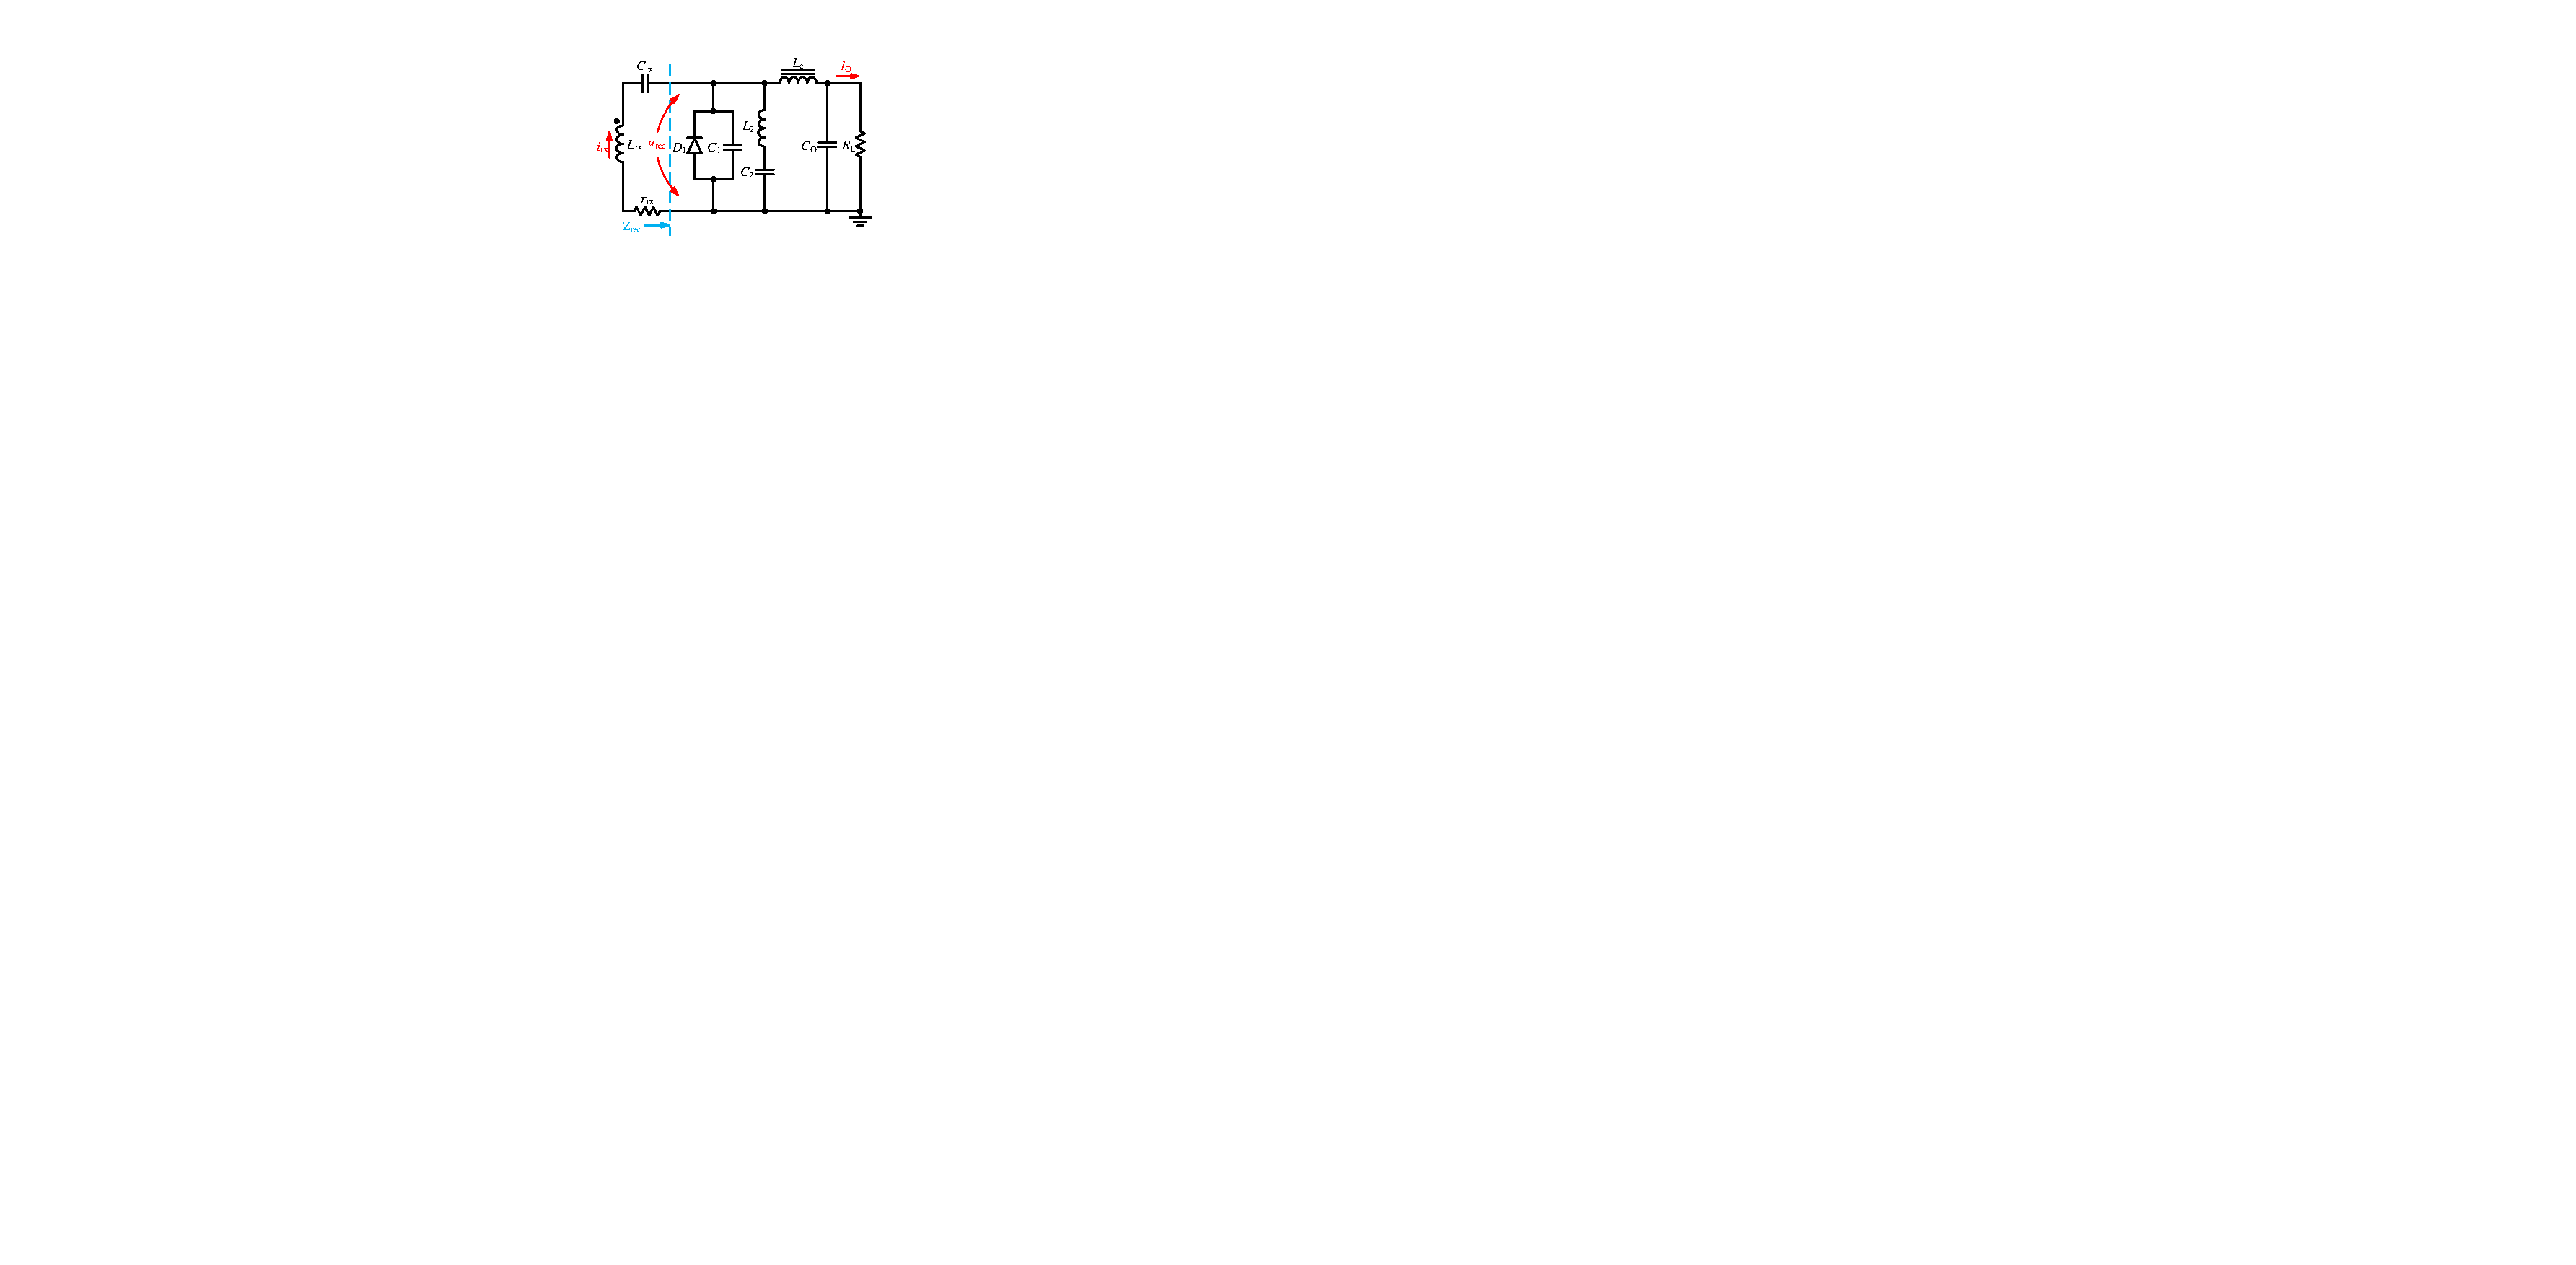
\includegraphics[width=2in]{FiguresEdge/RectifierEF.pdf}}
	\subfigure[]{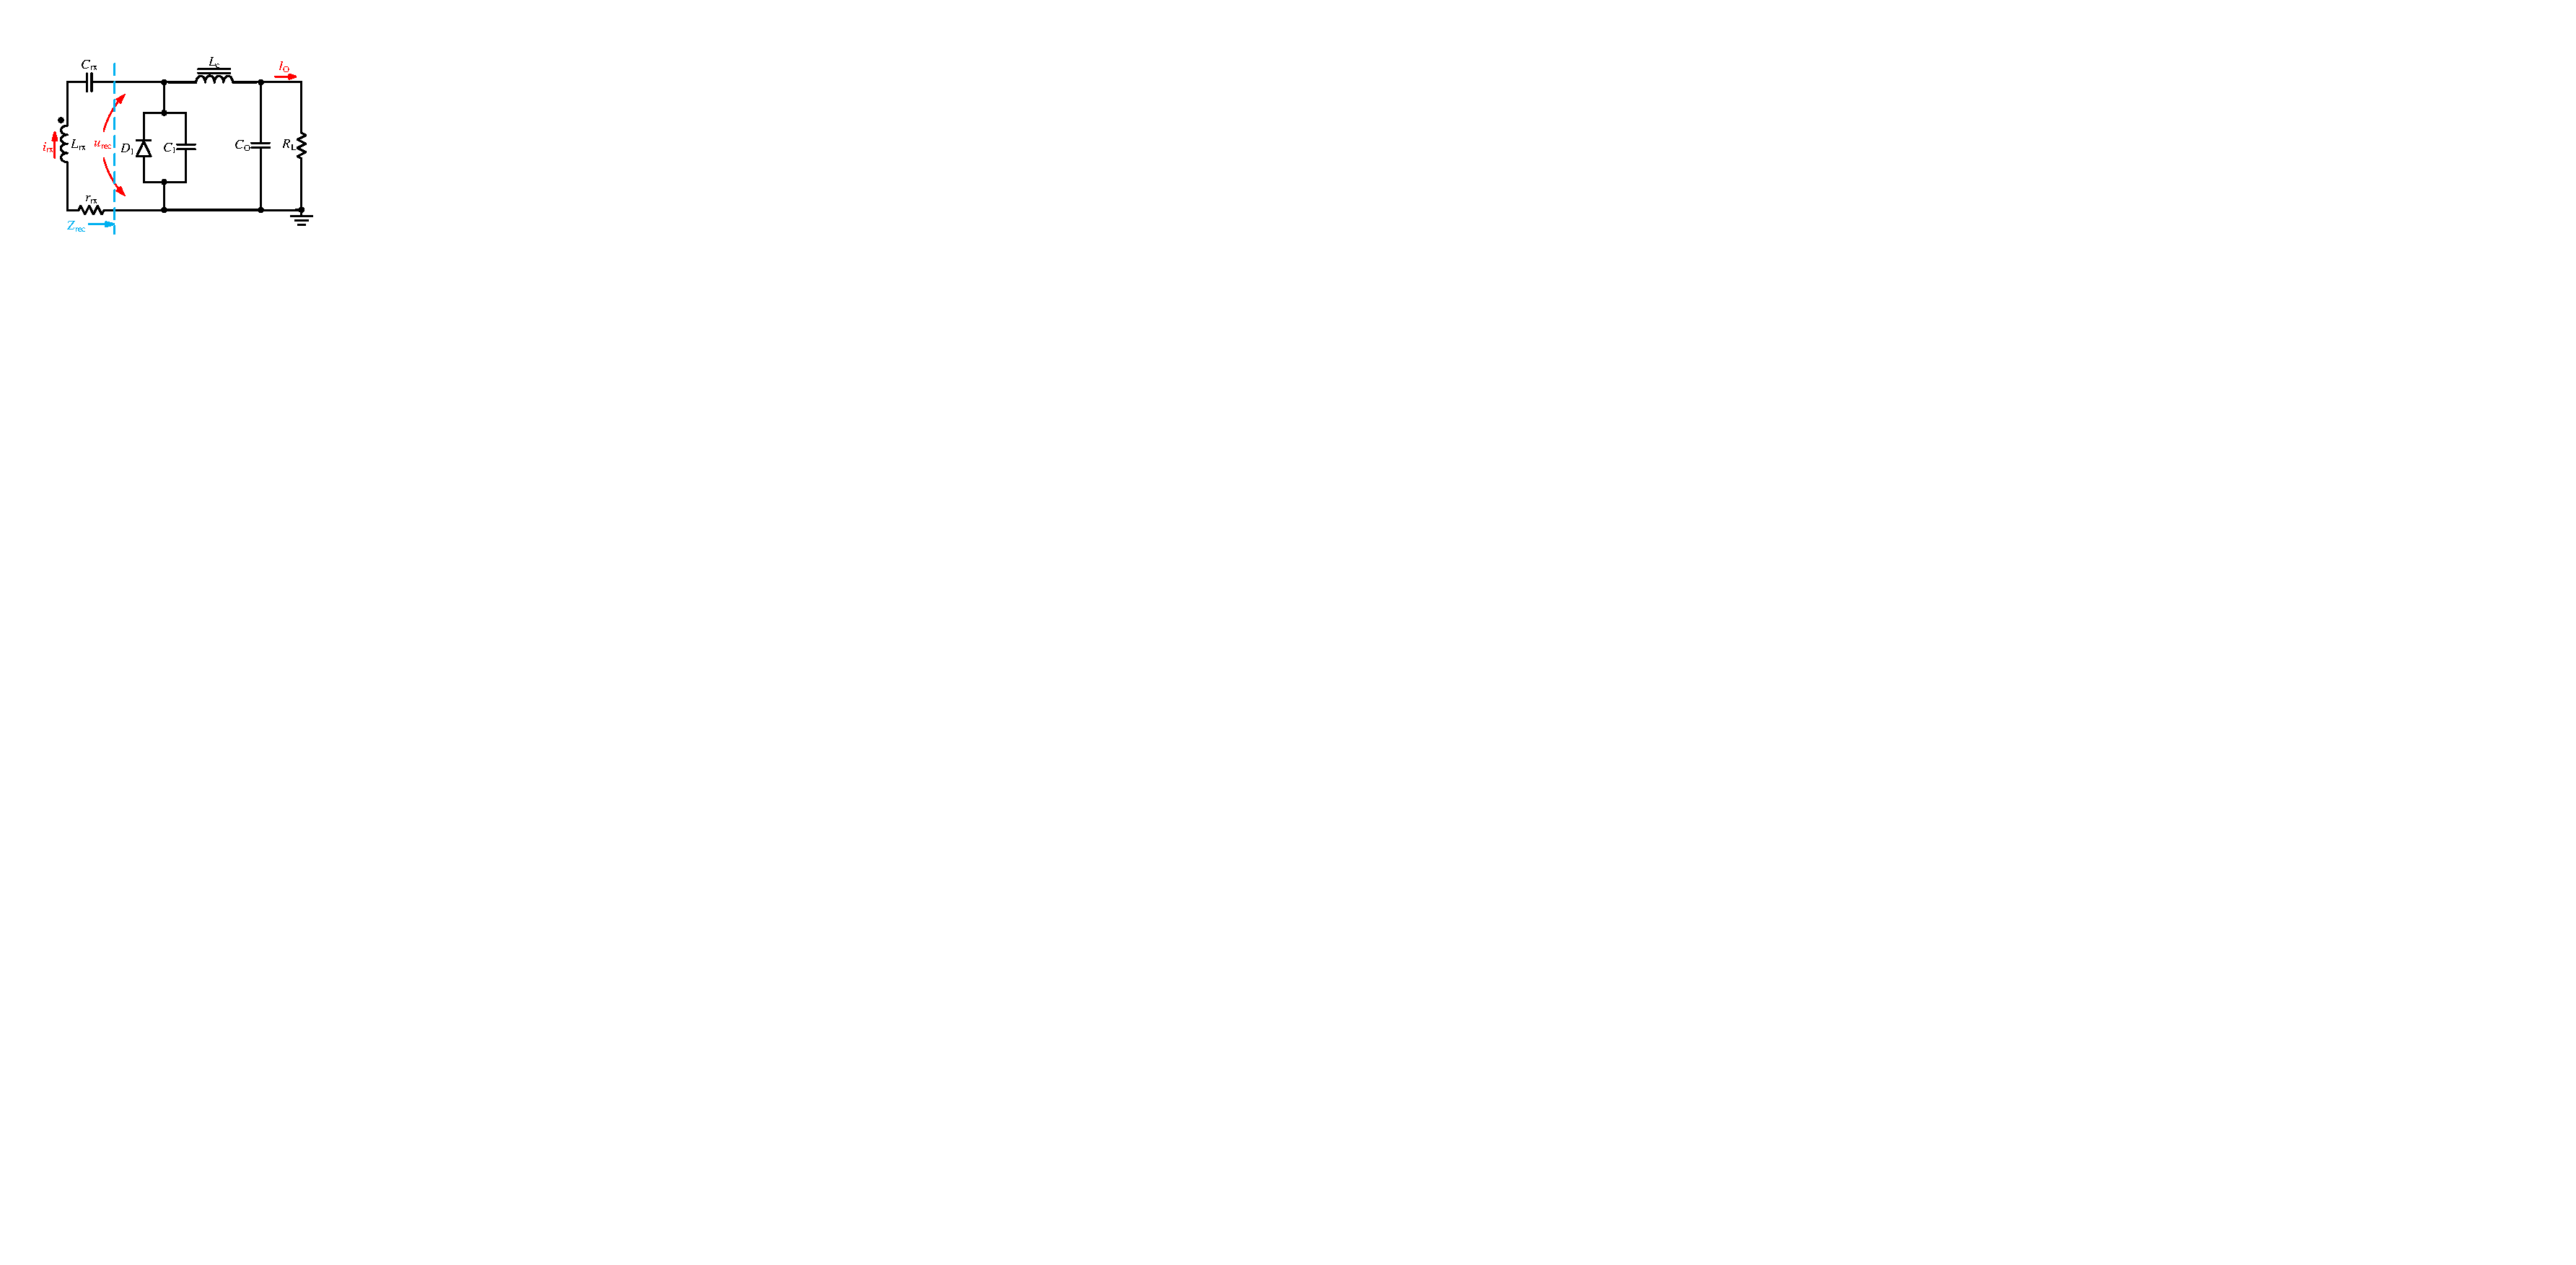
\includegraphics[width=2in]{FiguresEdge/RectifierHalfwave.pdf}}
	\caption{Class E family of rectifiers. (a) Full-wave rectifier. (b) Class EF rectifier. (c) Half-wave rectifier.}
	\label{fig:ClassEfamilyrectifier}
\end{figure}

\ifx\allfiles\undefined
	\onehalfspacing
	\bibliographystyle{chicago}
	%****************************************************************
	%=========This is the file that contains your bibliography entries=======
	%****************************************************************
	\bibliography{HuanBib}
	%=======================================================
	\end{document}
\fi

%\cleardoublepage
%\ifx\allfiles\undefined
	\include{Config} %deifne the using package and the paper layout
	\begin{document}
\else
	
\fi
\chapter{Chapter2 Name}
\section{Overview}
Here is the overview of chapter2. Here is the overview of chapter2. Here is the overview of chapter2. Here is the overview of chapter2

Here is the overview of chapter2. Here is the overview of chapter2. Here is the overview of chapter2. Here is the overview of chapter2

Here is the overview of chapter2. Here is the overview of chapter2. Here is the overview of chapter2. Here is the overview of chapter2

Here is the overview of chapter2. Here is the overview of chapter2. Here is the overview of chapter2. Here is the overview of chapter2

Here is the overview of chapter2. Here is the overview of chapter2. Here is the overview of chapter2. Here is the overview of chapter2

Here is the overview of chapter2. Here is the overview of chapter2. Here is the overview of chapter2. Here is the overview of chapter2

Here is the overview of chapter2. Here is the overview of chapter2. Here is the overview of chapter2. Here is the overview of chapter2

Here is the overview of chapter2. Here is the overview of chapter2. Here is the overview of chapter2. Here is the overview of chapter2
\begin{figure}[!htb]
	\centering
	\subfigure[]{\includegraphics[width=2in]{FiguresEdge/RectifierFullWave.pdf}}
	\subfigure[]{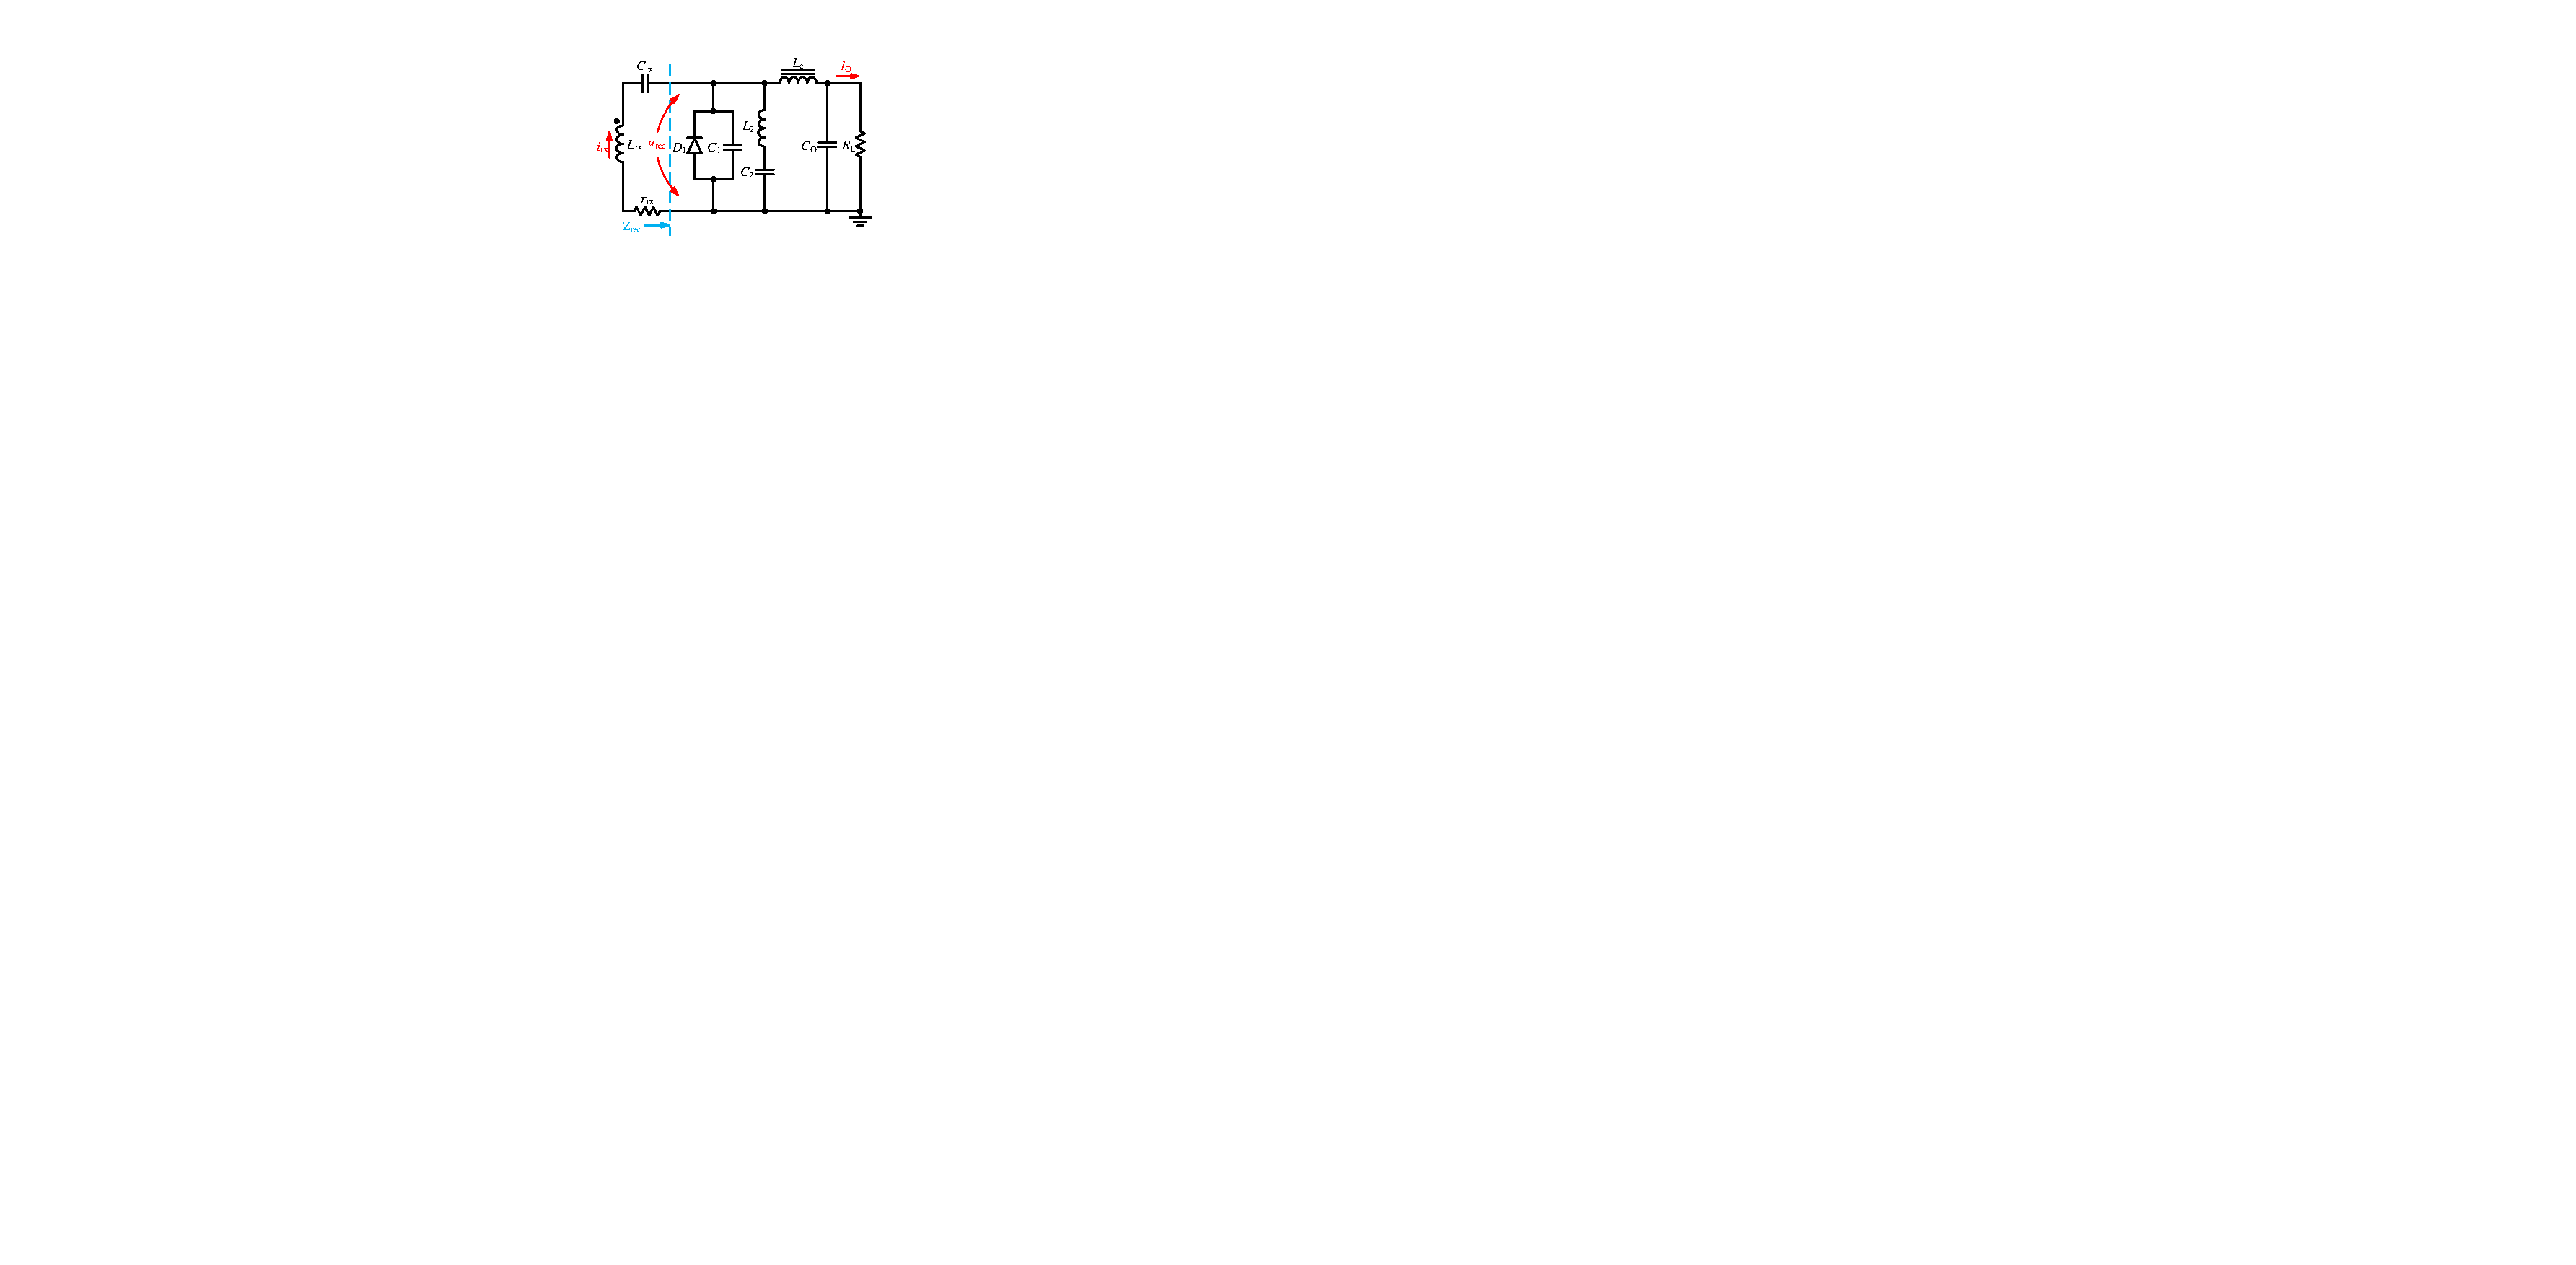
\includegraphics[width=2in]{FiguresEdge/RectifierEF.pdf}}
	\subfigure[]{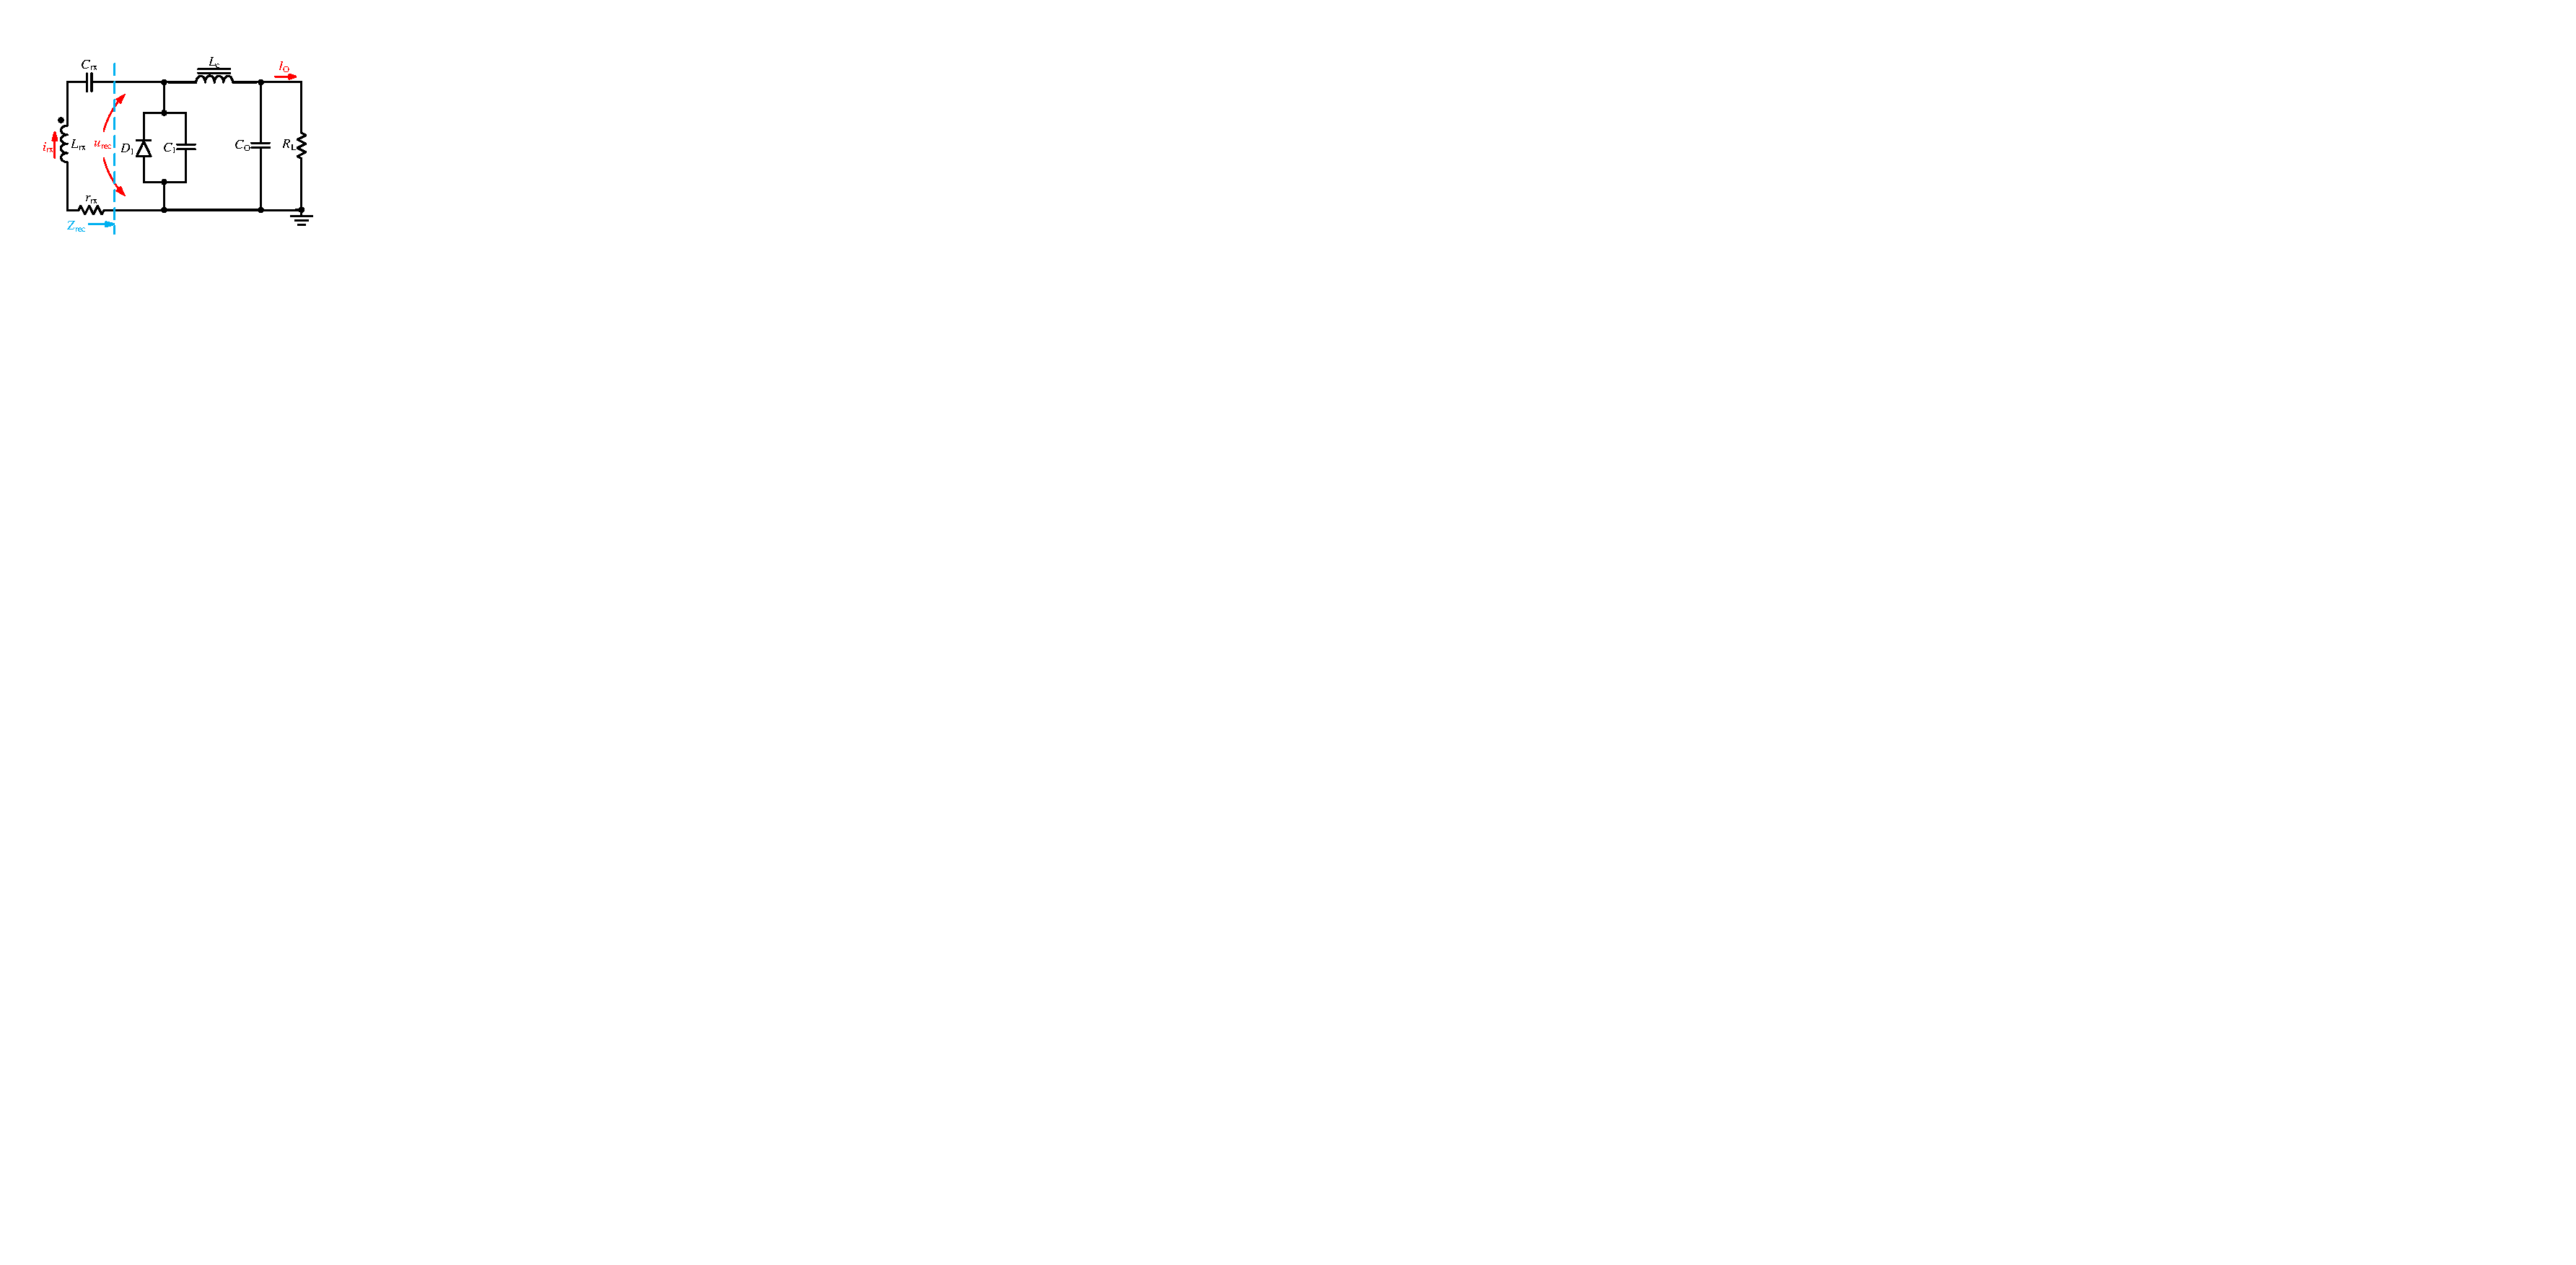
\includegraphics[width=2in]{FiguresEdge/RectifierHalfwave.pdf}}
	\caption{Class E family of rectifiers. (a) Full-wave rectifier. (b) Class EF rectifier. (c) Half-wave rectifier.}
	\label{fig:ClassEfamilyrectifier}
\end{figure}





\ifx\allfiles\undefined
	\onehalfspacing
	\bibliographystyle{chicago}
	%****************************************************************
	%=========This is the file that contains your bibliography entries=======
	%****************************************************************
	\bibliography{HuanBib}
	%=======================================================
	\end{document}
\fi=======================================

%\cleardoublepage
%%\ifx\allfiles\undefined
	\include{Config} %deifne the using package and the paper layout
	\begin{document}
\else
	
\fi
\chapter{Chapter3 Name}
\section{Overview}
Here is the overview of chapter3. Here is the overview of chapter3. Here is the overview of chapter3. Here is the overview of chapter3.

Here is the overview of chapter3. Here is the overview of chapter3. Here is the overview of chapter3. Here is the overview of chapter3.

Here is the overview of chapter3. Here is the overview of chapter3. Here is the overview of chapter3. Here is the overview of chapter3.

Here is the overview of chapter3. Here is the overview of chapter3. Here is the overview of chapter3. Here is the overview of chapter3.

Here is the overview of chapter3. Here is the overview of chapter3. Here is the overview of chapter3. Here is the overview of chapter3.

Here is the overview of chapter3. Here is the overview of chapter3. Here is the overview of chapter3. Here is the overview of chapter3.


\section{Section3}
\label{sec:ModularMRSystem}

\subsection{Modular Architecture}
ABCDE

\ifx\allfiles\undefined
	\onehalfspacing
	\bibliographystyle{chicago}
	%****************************************************************
	%=========This is the file that contains your bibliography entries=======
	%****************************************************************
	\bibliography{HuanBib}
	%=======================================================
	\end{document}
\fi
%%\cleardoublepage
%%\ifx\allfiles\undefined
	\include{Config}
	\begin{document}
\else
	
\fi
\chapter{Current Status and Working Plan}
\section{Overview}
Here is the overview. Here is the overview Here is the overview. Here is the overview. Here is the overview.

Here is the overview. Here is the overview Here is the overview. Here is the overview. Here is the overview

Here is the overview. Here is the overview Here is the overview. Here is the overview. Here is the overview

Here is the overview. Here is the overview Here is the overview. Here is the overview. Here is the overview

Here is the overview. Here is the overview Here is the overview. Here is the overview. Here is the overview

Here is the overview. Here is the overview Here is the overview. Here is the overview. Here is the overview
\section{Summary}\label{sec:Chapter4summary}
Here is the Summary.

\ifx\allfiles\undefined
	\onehalfspacing
	\bibliographystyle{chicago}
	%****************************************************************
	%=========This is the file that contains your bibliography entries=======
	%****************************************************************
	\bibliography{HuanBib}
	%=======================================================
	\end{document}
\fi



%%\cleardoublepage
%%\include{Chapter5}
%%\cleardoublepage
%\include{Conclusion}
%\cleardoublepage
%\chapter*{ACKNOWLEDGEMENT}

Here I would like to thank all the individuals who provide your kind supports and assistances to me and finally make this dissertation possible. It is hard to use words to express my gratitude to all of you.

Foremost, I want to express my heartfelt thanks to my Ph.D supervisor Prof.Chengbin Ma. His wisdom, knowledge, and encouragement really make me to mature as a qualified researcher.
Without his guidance, it is hard for me to make all the accomplishments what I have already achieved. 

Moreover, I would like to express my gratitude to my dissertation committee members, Prof. Houjun Tang, Prof. Jigang Wu, Prof. Mian Li, and Prof. Xinen Zhu. Their detailed guidance and insightful comments are very helpful to further improve the quality of this dissertation and make it more solid, both in terms of technical contents and readability. Also, many thanks to Prof. Patrick Chi-Kwong LUK and Dr. Songnan Yang for their worthful guidance and advice on my research works, especially at the very beginning of my research.

And then, I am grateful to all my lab mates for their selfless helps. I am very enjoy the time working with them all. I also thank the JI staffs for your kind supports throughout my Ph.D program.

Finally, I want to give the special thanks to my family, especially my wife and my son. I will never forget the debt I owe you for your gratuitous support and understanding in the past three years. For this sake, I dedicate the dissertation to you.





%\cleardoublepage
%\include{Appendix}
%\cleardoublepage
%\onehalfspacing
%\bibliographystyle{chicago}
%%****************************************************************
%%=========This is the file that contains your bibliography entries=======
%%****************************************************************
%\bibliography{References}
%%=======================================================
%\end{document}
 %deifne the using package and the paper layout
	\begin{document}
\else

\fi

\chapter{Introduction}
\section{Overview}
Here is the background~\citep{MHzcompact}
Here is the overview of chapter1. Here is the overview of chapter1. Here is the overview of chapter1. Here is the overview of CSD. 

Here is the overview of chapter1. Here is the overview of chapter1. Here is the overview of chapter1. Here is the overview of chapter1

Here is the overview of chapter1. Here is the overview of chapter1. Here is the overview of chapter1. Here is the overview of chapter1

Here is the overview of chapter1. Here is the overview of chapter1. Here is the overview of chapter1. Here is the overview of chapter1

Here is the overview of chapter1. Here is the overview of chapter1. Here is the overview of chapter1. Here is the overview of chapter1

Here is the overview of chapter1. Here is the overview of chapter1. Here is the overview of chapter1. Here is the overview of chapter1

Here is the overview of chapter1. Here is the overview of chapter1. Here is the overview of chapter1. Here is the overview of BAC

Here is the overview of chapter1. Here is the overview of chapter1. Here is the overview of chapter1. Here is the overview of chapter1

\begin{figure}[!htb]
	\centering
	\subfigure[]{\includegraphics[width=2in]{FiguresEdge/RectifierFullWave.pdf}}
	\subfigure[]{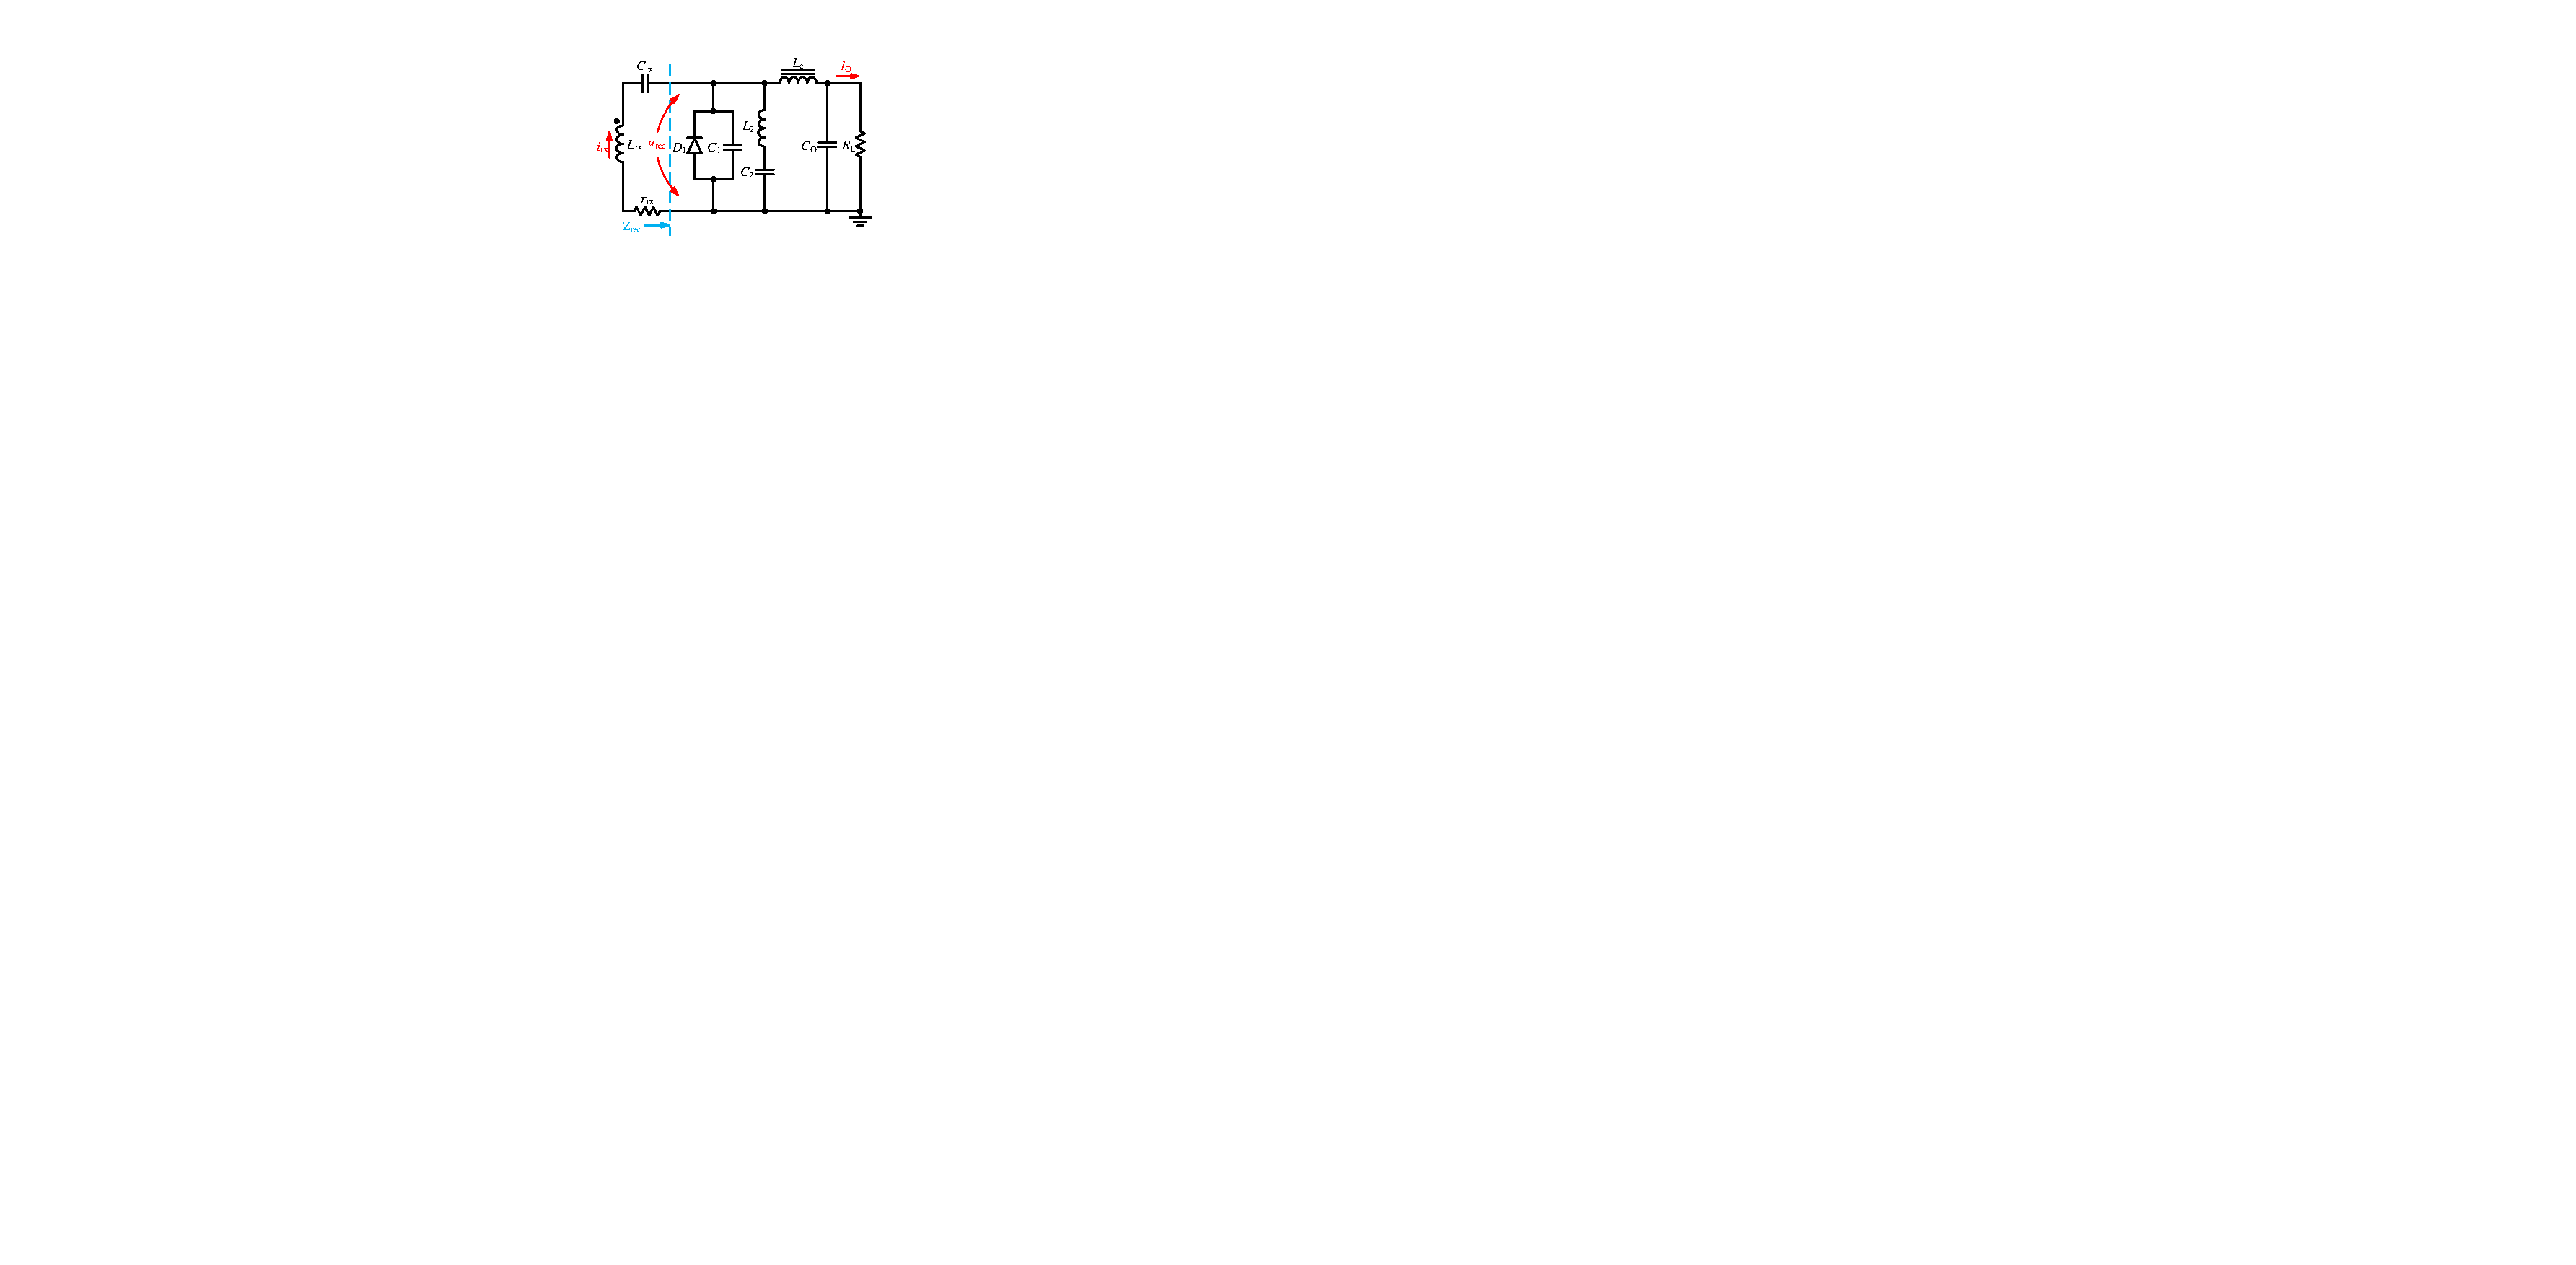
\includegraphics[width=2in]{FiguresEdge/RectifierEF.pdf}}
	\subfigure[]{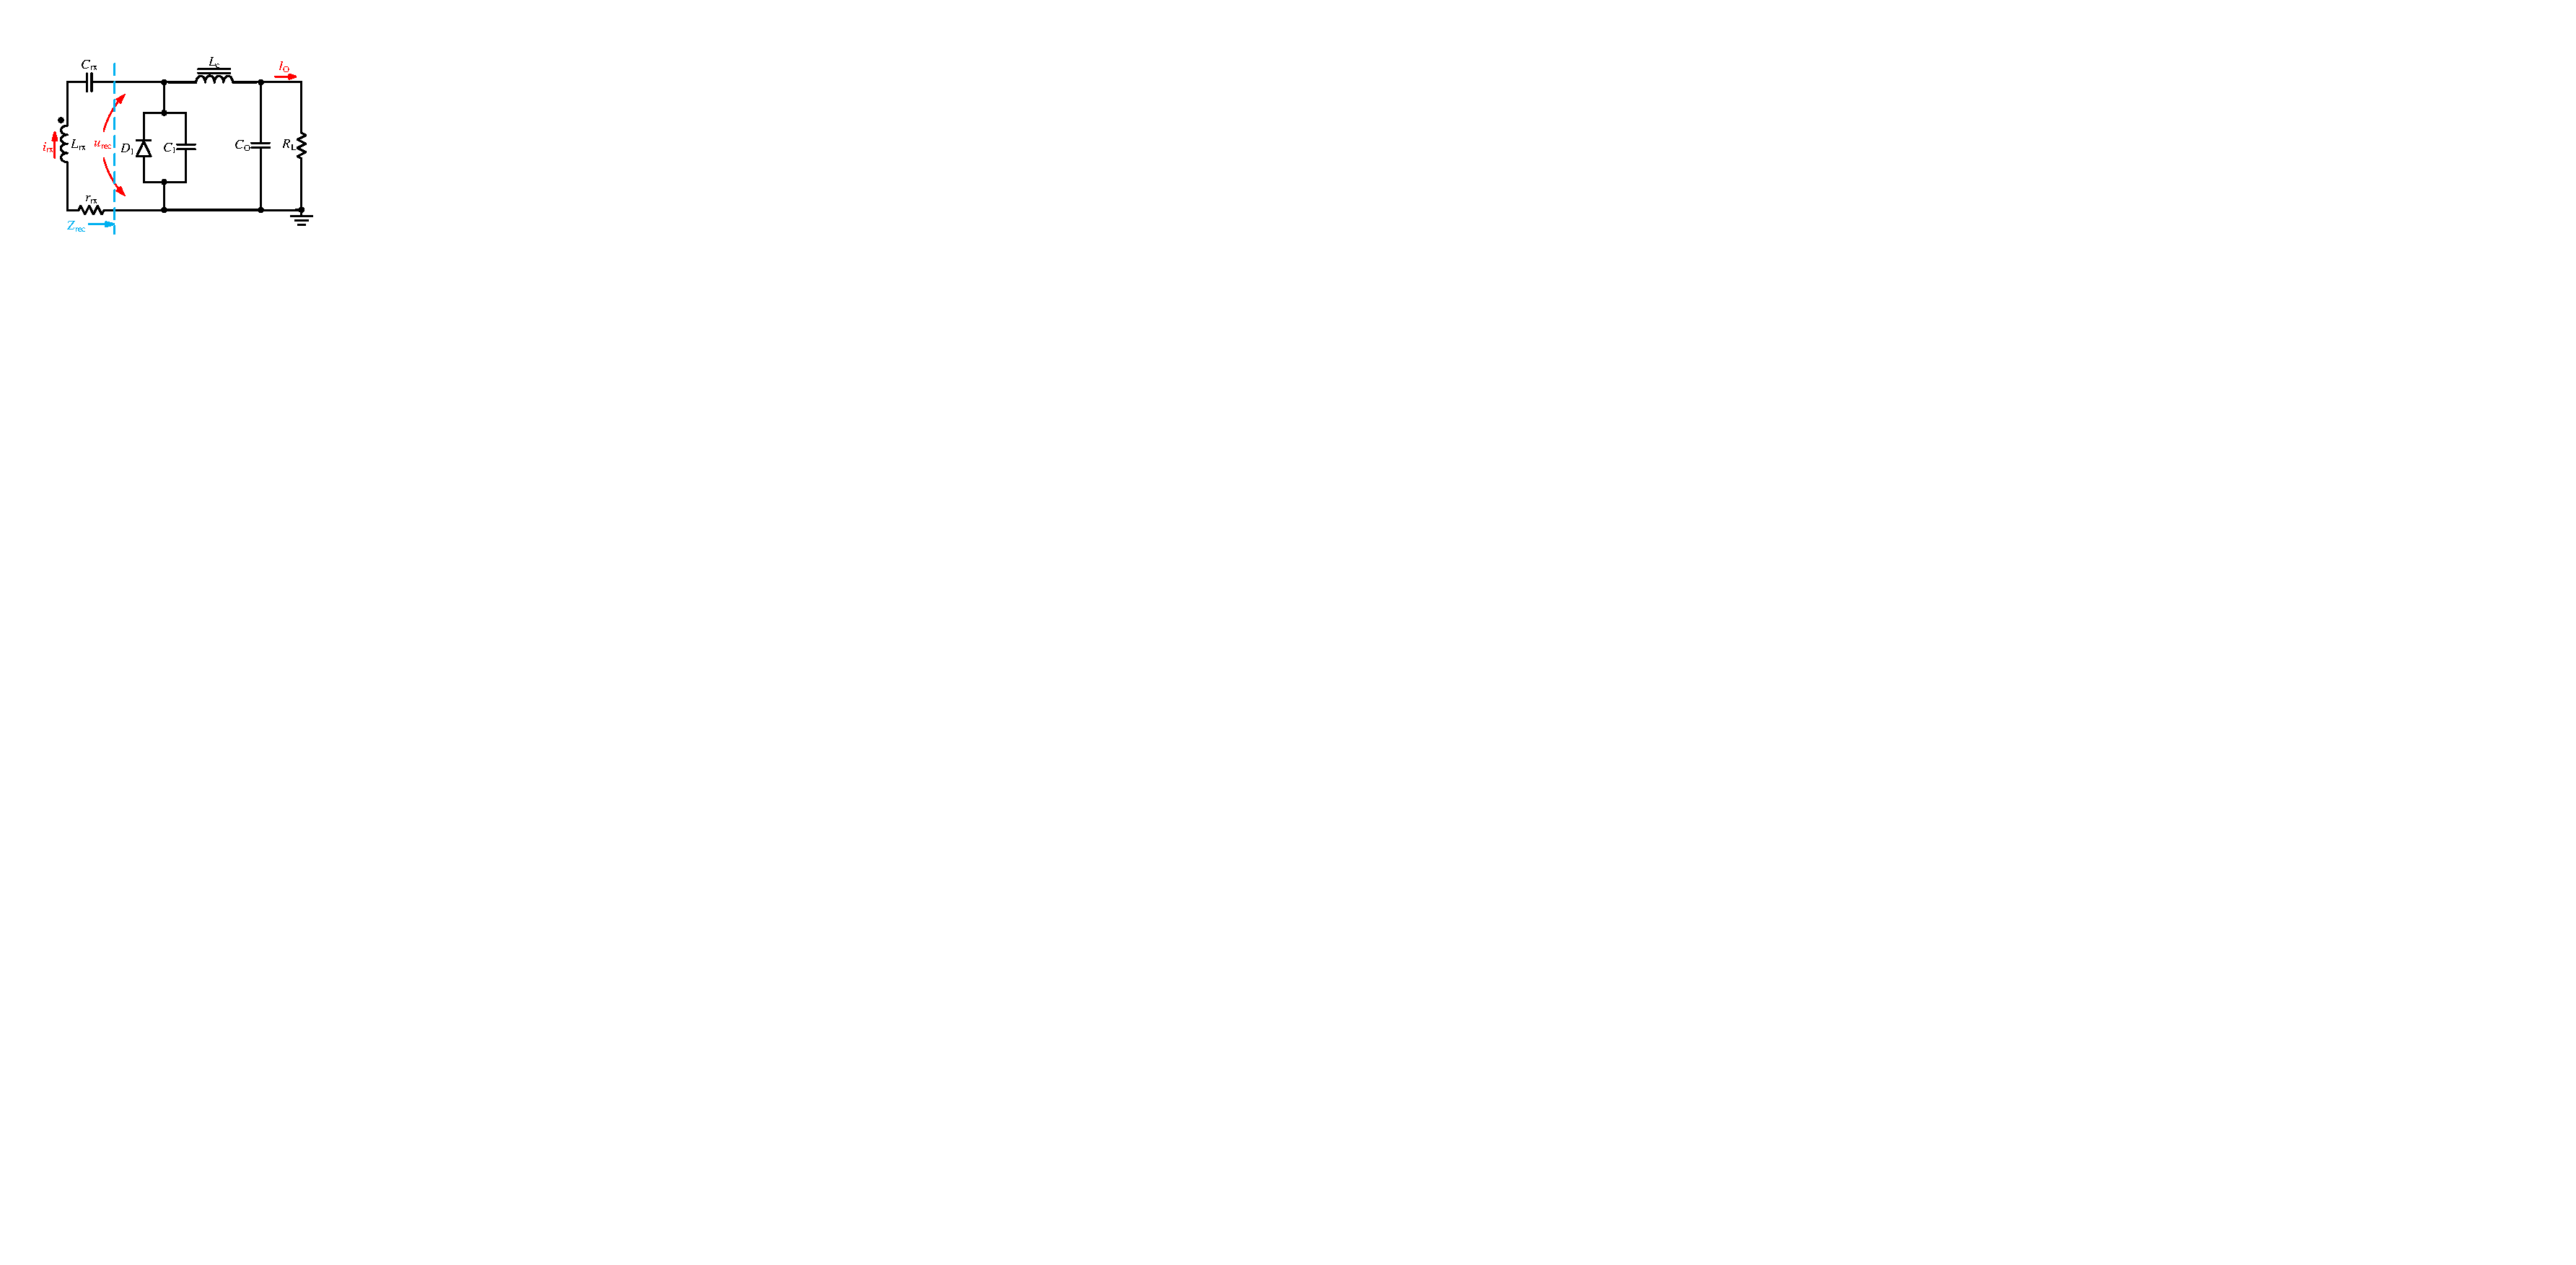
\includegraphics[width=2in]{FiguresEdge/RectifierHalfwave.pdf}}
	\caption{Class E family of rectifiers. (a) Full-wave rectifier. (b) Class EF rectifier. (c) Half-wave rectifier.}
	\label{fig:ClassEfamilyrectifier}
\end{figure}

\ifx\allfiles\undefined
	\onehalfspacing
	\bibliographystyle{chicago}
	%****************************************************************
	%=========This is the file that contains your bibliography entries=======
	%****************************************************************
	\bibliography{HuanBib}
	%=======================================================
	\end{document}
\fi

%\cleardoublepage
%\ifx\allfiles\undefined
	\documentclass[12pt,a4paper,twoside,openright]{report}
%
%-----Packages
%
\usepackage[english]{babel}
\usepackage{setspace}
\usepackage[T1]{fontenc}
\usepackage[latin1]{inputenc}
\usepackage[intlimits]{amsmath}
\usepackage{amsfonts,amssymb}
\usepackage{natbib}
\usepackage[normalsize,bf]{caption}
\usepackage[dvips]{graphicx}
\usepackage{color}
\usepackage[breaklinks,linktocpage]{hyperref}
\usepackage{fancyhdr}
\usepackage{setspace}
\usepackage{subfigure}
\usepackage{float}
\usepackage{lettrine}
\usepackage{comment}
\usepackage{pifont}
\usepackage{soul, color}  %\hl
\usepackage{booktabs}	  %\toprule in table
\usepackage{tabularx}	  %\tabular
\usepackage{multicol}	  %table col
\usepackage{multirow}	  %table row
\usepackage{diagbox}

\newcommand{\hlg}[2][green]{{\sethlcolor{#1}\hl{#2}}}
\newcommand{\tabincell}[2]{\begin{tabular}{@{}#1@{}}#2\end{tabular}}
\sloppy\par
%****************************************************************
% ===========Optional packages (uncomment as needed)=============
%****************************************************************
\usepackage{wrapfig}
%\usepackage{makeidx}
\usepackage{amsbsy}
\usepackage{latexsym}
\usepackage{amsthm}
\usepackage{datatool}
%\usepackage{glossary}
\usepackage{glossaries}
%\makeglossary
%\makeglossaries


%=======================================================
%
%-----Layout
%
\onehalfspacing
\hoffset = -1 in
\voffset= -1 in
%
%-----Set margins for a4 paper
%
\topmargin = 3.0cm
\textwidth = 17cm
\textheight = 22cm
\oddsidemargin =  2cm
\evensidemargin = 2cm
%
%-----Headers and Footers
%
\pagestyle{fancyplain}
\renewcommand{\chaptermark}[1]%
{\markboth{#1}{}}
\renewcommand{\sectionmark}[1]%
{\markright{\thesection\ -- #1}}
\lhead[\fancyplain{}{\thepage}]%
{\fancyplain{}{\rightmark}}
\rhead[\fancyplain{}{\leftmark}]%
{\fancyplain{}{\thepage}}
\cfoot{}
%
%-----No headers on empty pages before new chapter
%
\makeatletter
\def\cleardoublepage{\clearpage\if@twoside \ifodd\c@page\else
	\hbox{}
	\thispagestyle{plain}
	\newpage
	\if@twocolumn\hbox{}\newpage\fi\fi\fi}
\makeatother \clearpage{\pagestyle{plain}\cleardoublepage}
%
%-----Footnotes
%
\renewcommand{\thefootnote}{\fnsymbol{footnote}} % Footnotes are marked with symbols instead of literals
\setlength{\textfloatsep}{8pt plus 4pt minus 4pt}        % Separation of floats from text
\renewcommand{\bibnumfmt}[1]{{\scriptsize #1}}
\setlength{\bibhang}{2em}
%
%-----Define Horizontal rule
%
\newcommand{\HRule}{\rule{\textwidth}{0.5mm}}
%
%-----Define Hyperlink colors
%
\definecolor{darkred}{rgb}{0.25,0,0}
\definecolor{darkgreen}{rgb}{0,0.25,0}
\definecolor{darkblue}{rgb}{0,0,0.5}
\hypersetup{colorlinks,linkcolor=black,filecolor=black,urlcolor=darkblue,citecolor=black}
\usepackage{breakurl}
%****************************************************************
% ===========Add user definitions as needed=====================
%****************************************************************
%\include{definitions}
\newtheorem{theorem}{Theorem}[chapter]
\newtheorem{principle}{Principle}[chapter]
\newtheorem{algorithm}{Algorithm}[chapter]
\newtheorem{law}{Law}
%\theoremstyle{plain}  % Default
\theoremstyle{definition}
%\theoremstyle{remark}
\newtheorem{problem}{Problem}[chapter]
\newtheorem{example}{Example}[chapter]
\newtheorem{definition}{Definition}[chapter]




%%***********Config file orginal backup*********
%\immediate\write18{makeindex \jobname.nlo -s nomencl.ist -o \jobname.nls}
%\documentclass[12pt,a4paper,twoside,openright]{report}
%%
%%-----Packages
%%
%\usepackage[english]{babel}
%\usepackage{setspace}
%\usepackage[T1]{fontenc}
%\usepackage[latin1]{inputenc}
%\usepackage[intlimits]{amsmath}
%\usepackage{amsfonts,amssymb}
%\usepackage{natbib}
%\usepackage[normalsize,bf]{caption}
%\usepackage[dvips]{graphicx}
%%\usepackage{color}
%%\usepackage{mathdots}
%%\usepackage{mathtools}
%%\usepackage{booktabs}
%%\usepackage{multirow}
%%\usepackage{ps2pdf}
%\usepackage{epstopdf}
%\usepackage[breaklinks,linktocpage]{hyperref}
%\usepackage{fancyhdr}
%\usepackage{setspace}
%\usepackage{subfigure}
%\usepackage{lettrine}
%\newcommand{\tabincell}[2]{\begin{tabular}{@{}#1@{}}#2\end{tabular}}
%\sloppy\par
%%****************************************************************
%% ===========Optional packages (uncomment as needed)=============
%%****************************************************************
%\usepackage{wrapfig}
%%\usepackage{makeidx}
%\usepackage{amsbsy}
%\usepackage{latexsym}
%\usepackage{amsthm}
%\usepackage{datatool}
%\usepackage{nomencl}
%\makenomenclature
%\usepackage{glossaries}
%\makeglossaries
%\usepackage{ifthen}
%\usepackage{graphicx}
%\usepackage{color, soul}
%%\usepackage{wasysym}
%%\usepackage{psfrag}
%%\usepackage{subfig}
%%\usepackage{pifont}
%%\usepackage{longtable}
%%\setlength\LTleft{0pt}
%%\setlength\LTright{0pt}
%%=======================================================
%%
%%-----Layout
%%
%\onehalfspacing
%\hoffset = -1 in
%\voffset= -1 in
%%
%%-----Set margins for a4 paper
%%
%\topmargin = 3.0cm
%\textwidth = 17cm
%\textheight = 22cm
%\oddsidemargin =  2cm
%\evensidemargin = 2cm
%%
%%-----Headers and Footers
%%
%\pagestyle{fancyplain}
%\renewcommand{\chaptermark}[1]%
%            {\markboth{#1}{}}
%\renewcommand{\sectionmark}[1]%
%            {\markright{\thesection\ -- #1}}
%\lhead[\fancyplain{}{\thepage}]%
%      {\fancyplain{}{\rightmark}}
%\rhead[\fancyplain{}{\leftmark}]%
%     {\fancyplain{}{\thepage}}
%\cfoot{}
%%
%%-----No headers on empty pages before new chapter
%%
%\makeatletter
%\def\cleardoublepage{\clearpage\if@twoside \ifodd\c@page\else
%    \hbox{}
%    \thispagestyle{plain}
%    \newpage
%    \if@twocolumn\hbox{}\newpage\fi\fi\fi}
%\makeatother \clearpage{\pagestyle{plain}\cleardoublepage}
%%
%%-----Footnotes
%%
%\renewcommand{\thefootnote}{\fnsymbol{footnote}} % Footnotes are marked with symbols instead of literals
%\setlength{\textfloatsep}{8pt plus 4pt minus 4pt}        % Separation of floats from text
%\renewcommand{\bibnumfmt}[1]{{\scriptsize #1}}
%\setlength{\bibhang}{2em}
%%
%%-----Define Horizontal rule
%%
%\newcommand{\HRule}{\rule{\textwidth}{0.5mm}}
%%
%%-----Define Hyperlink colors
%%
%\definecolor{darkred}{rgb}{0.25,0,0}
%\definecolor{darkgreen}{rgb}{0,0.25,0}
%\definecolor{darkblue}{rgb}{0,0,0.5}
%\hypersetup{colorlinks,linkcolor=black,filecolor=black,urlcolor=darkblue,citecolor=black}
%\usepackage{breakurl}
%
%%****************************************************************
%% ===========Add user definitions as needed=====================
%%****************************************************************
%\include{definitions}
%\newtheorem{theorem}{Theorem}[chapter]
%\newtheorem{principle}{Principle}[chapter]
%%\newtheorem{algorithm}{Algorithm}[chapter]
%\newtheorem{law}{Law}
%%\theoremstyle{plain}  % Default
%\theoremstyle{definition}
%%\theoremstyle{remark}
%\newtheorem{problem}{Problem}[chapter]
%\newtheorem{example}{Example}[chapter]
%\newtheorem{definition}{Definition}[chapter]
%%=======================================================
%%%%%%%%%%%%%
%%-----Begin Document
%%%%%%%%%%%%%
%\begin{document}
%\pagenumbering{roman}
%%
%%-----Title page
%%
%
%\begin{titlepage}
%\noindent {\bf Shanghai Jiao Tong University \\
%University of Michigan- Shanghai Jiao Tong University Joint Institute}\\
%\noindent \HRule \vspace{0.0455\textheight}
%%****************************************************************
%% ===========Edit the following lines to get the right title============
%%****************************************************************
%\begin{center}
%{\huge \bf Proposal Name}\\[0.016\textheight]
%{\Large \bf Doctoral Dissertation Proposal} \\[0.032\textheight]
%\large{by} \\[0.032\textheight] \Large{ \bf Jibin Song}\\
%%=======================================================
%\vspace{5cm}
%\normalsize{A proposal submitted in satisfaction of the \\
%requirements for the degree of Doctor of Philosophy in \\
%Control Science and Engineering at Shanghai Jiao Tong University}
%\HRule \\[0.023\textheight]
%%****************************************************************
%%======Edit the following lines to get the right committee members======
%%****************************************************************
%\begin{tabular*}{\textwidth}{@{}l@{\extracolsep{\fill}}r@{}}
%\textbf{Committee in charge:} &  \textbf{Shanghai}\\
%\textbf{Professor XXX} &  \textbf{July, 2020}\\
%\textbf{Professor XXX} & \\
%\textbf{Professor XXX} & \\
%\textbf{Professor XXX} & \\
%\textbf{Professor XXX} & \\
%\end{tabular*}
%%=======================================================
%\end{center}
%\end{titlepage}
%
%%
%%-----Abstract
%%
%\thispagestyle{empty}
%\cleardoublepage
%%****************************************************************
%%===========Your abstract goes in the file Abstract.tex==============
%%****************************************************************
%
%
%
%\begin{abstract}
\noindent

Here is the abstract. Here is the abstract. Here is the abstract. Here is the abstract.

Here is the abstract. Here is the abstract. Here is the abstract. Here is the abstract.

Here is the abstract. Here is the abstract. Here is the abstract. Here is the abstract.

Here is the abstract. Here is the abstract. Here is the abstract. Here is the abstract.

Here is the abstract. Here is the abstract. Here is the abstract. Here is the abstract.

Here is the abstract. Here is the abstract. Here is the abstract. Here is the abstract.

Here is the abstract. Here is the abstract. Here is the abstract. Here is the abstract.

Here is the abstract. Here is the abstract. Here is the abstract. Here is the abstract.
\end{abstract}



%\cleardoublepage
%\newlength{\nomitemorigsep}
\setlength{\nomitemorigsep}{\nomitemsep}
\setlength{\nomitemsep}{-\parsep}
\makenomenclature
\renewcommand{\nomgroup}[1]{%
  \itemsep\nomitemorigsep%
  \ifthenelse{%
    \equal{#1}{A}%
  }{%
  \item[\textbf{Abbreviations}]%

  }{%
    \ifthenelse{\equal{#1}{S}}{%
    \item[\textbf{List of Symbols}]%

    }{}%
  }%
  \itemsep\nomitemsep
}
\renewcommand{\nomname}{Nomenclature}
\markboth{\MakeUppercase\nomname}{\MakeUppercase\nomname}
\printnomenclature[0.8in]
\nomenclature[A]{ADS}{Advanced Design System}
\nomenclature[A]{ESR}{Equivalent series resistance}
\nomenclature[A]{MOSFET}{Metal-oxide-semiconductor field effect transistor}
\nomenclature[A]{MWPT}{Multiple-receiver wrieless power transfer}
\nomenclature[A]{PA}{Power amplifier}
\nomenclature[A]{RF}{Radio frequency}
\nomenclature[A]{SRR}{Synchronous Resonant Rectifier}
\nomenclature[A]{WPT}{Wireless power transfer}
\nomenclature[A]{ZVS}{Zero-voltage-switching}




\nomenclature[S]{$C_{0}$}{Capacitor in resonant tank of Class E PA}
\nomenclature[S]{$C_{r}$}{Diode/switch shunt capacitor of Class E rectifier}
\nomenclature[S]{$C_{S}$}{Switch shunt capacitor of Class E PA}
\nomenclature[S]{$C_{rx}$}{Compensation capacitor of receiving coil}
\nomenclature[S]{$C_{tx}$}{Compensation capacitor of transmitting coil}
\nomenclature[S]{$k$}{Mutual inductance coefficient of coupling coils}
\nomenclature[S]{$k_{ij}$}{Mutual inductance coefficient between $i$-th and $j$-th coils in MWPT}
\nomenclature[S]{$L_{0}$}{Inductor in resonant tank of Class E PA}
\nomenclature[S]{$L_{rx}$}{Inductance of receiving coil}
\nomenclature[S]{$L_{tx}$}{Inductance of transmitting coil}
\nomenclature[S]{$M$}{Mutual inductance of coupling coils}
\nomenclature[S]{$M_{ij}$}{Mutual inductance between $i$-th and $j$-th coils in MWPT}
\nomenclature[S]{$r_{rx}$}{ESR of receiving coil}
\nomenclature[S]{$r_{tx}$}{ESR of transmitting coil}
\nomenclature[S]{$R_{L}$}{Dc load of rectifier}
\nomenclature[S]{$R_{rec}$}{Input resisance of rectifier}
\nomenclature[S]{$v_{DS}$}{Drain-source voltage of MOSFET}
\nomenclature[S]{$v_{GS}$}{Gate-source voltage of MOSFET}
\nomenclature[S]{$X_{rec}$}{Input reactance of rectifier}
\nomenclature[S]{$Z_{rec}$}{Input impedance of rectifier}
\nomenclature[S]{$Z_{coil}$}{Input impedance of transmitting coil}
\nomenclature[S]{$\eta_{PA}$}{Efficiency of PA}
\nomenclature[S]{$\eta_{rec}$}{Efficiency of rectifier}
\nomenclature[S]{$\eta_{sys}$}{Dc-dc efficiency of WPT system}
\nomenclature[S]{$\eta_{coil2load}$}{Power transfer efficiency from transmitting coil to dc load}


\cleardoublepage 







%\cleardoublepage
%%\printglossary
%%=======================================================
%%
%%-----Table of contents
%%
%%\clearpage
%\setcounter{tocdepth}{1}
%\setcounter{page}{1}
%\tableofcontents
%\doublespacing
%\listoffigures
%\doublespacing
%\listoftables
%\doublespacing
%
%
%
%
%
%\setcounter{page}{1}
%\pagenumbering{arabic}
%%****************************************************************
%%================Include each chapter in a different file===========
%%======For large theses, chapters should be in different directories=======
%%=============Add \cleardoublepage between each chapter==========
%%****************************************************************
%\ifx\allfiles\undefined   
	\include{Config} %deifne the using package and the paper layout
	\begin{document}
\else

\fi

\chapter{Introduction}
\section{Overview}
Here is the background~\citep{MHzcompact}
Here is the overview of chapter1. Here is the overview of chapter1. Here is the overview of chapter1. Here is the overview of CSD. 

Here is the overview of chapter1. Here is the overview of chapter1. Here is the overview of chapter1. Here is the overview of chapter1

Here is the overview of chapter1. Here is the overview of chapter1. Here is the overview of chapter1. Here is the overview of chapter1

Here is the overview of chapter1. Here is the overview of chapter1. Here is the overview of chapter1. Here is the overview of chapter1

Here is the overview of chapter1. Here is the overview of chapter1. Here is the overview of chapter1. Here is the overview of chapter1

Here is the overview of chapter1. Here is the overview of chapter1. Here is the overview of chapter1. Here is the overview of chapter1

Here is the overview of chapter1. Here is the overview of chapter1. Here is the overview of chapter1. Here is the overview of BAC

Here is the overview of chapter1. Here is the overview of chapter1. Here is the overview of chapter1. Here is the overview of chapter1

\begin{figure}[!htb]
	\centering
	\subfigure[]{\includegraphics[width=2in]{FiguresEdge/RectifierFullWave.pdf}}
	\subfigure[]{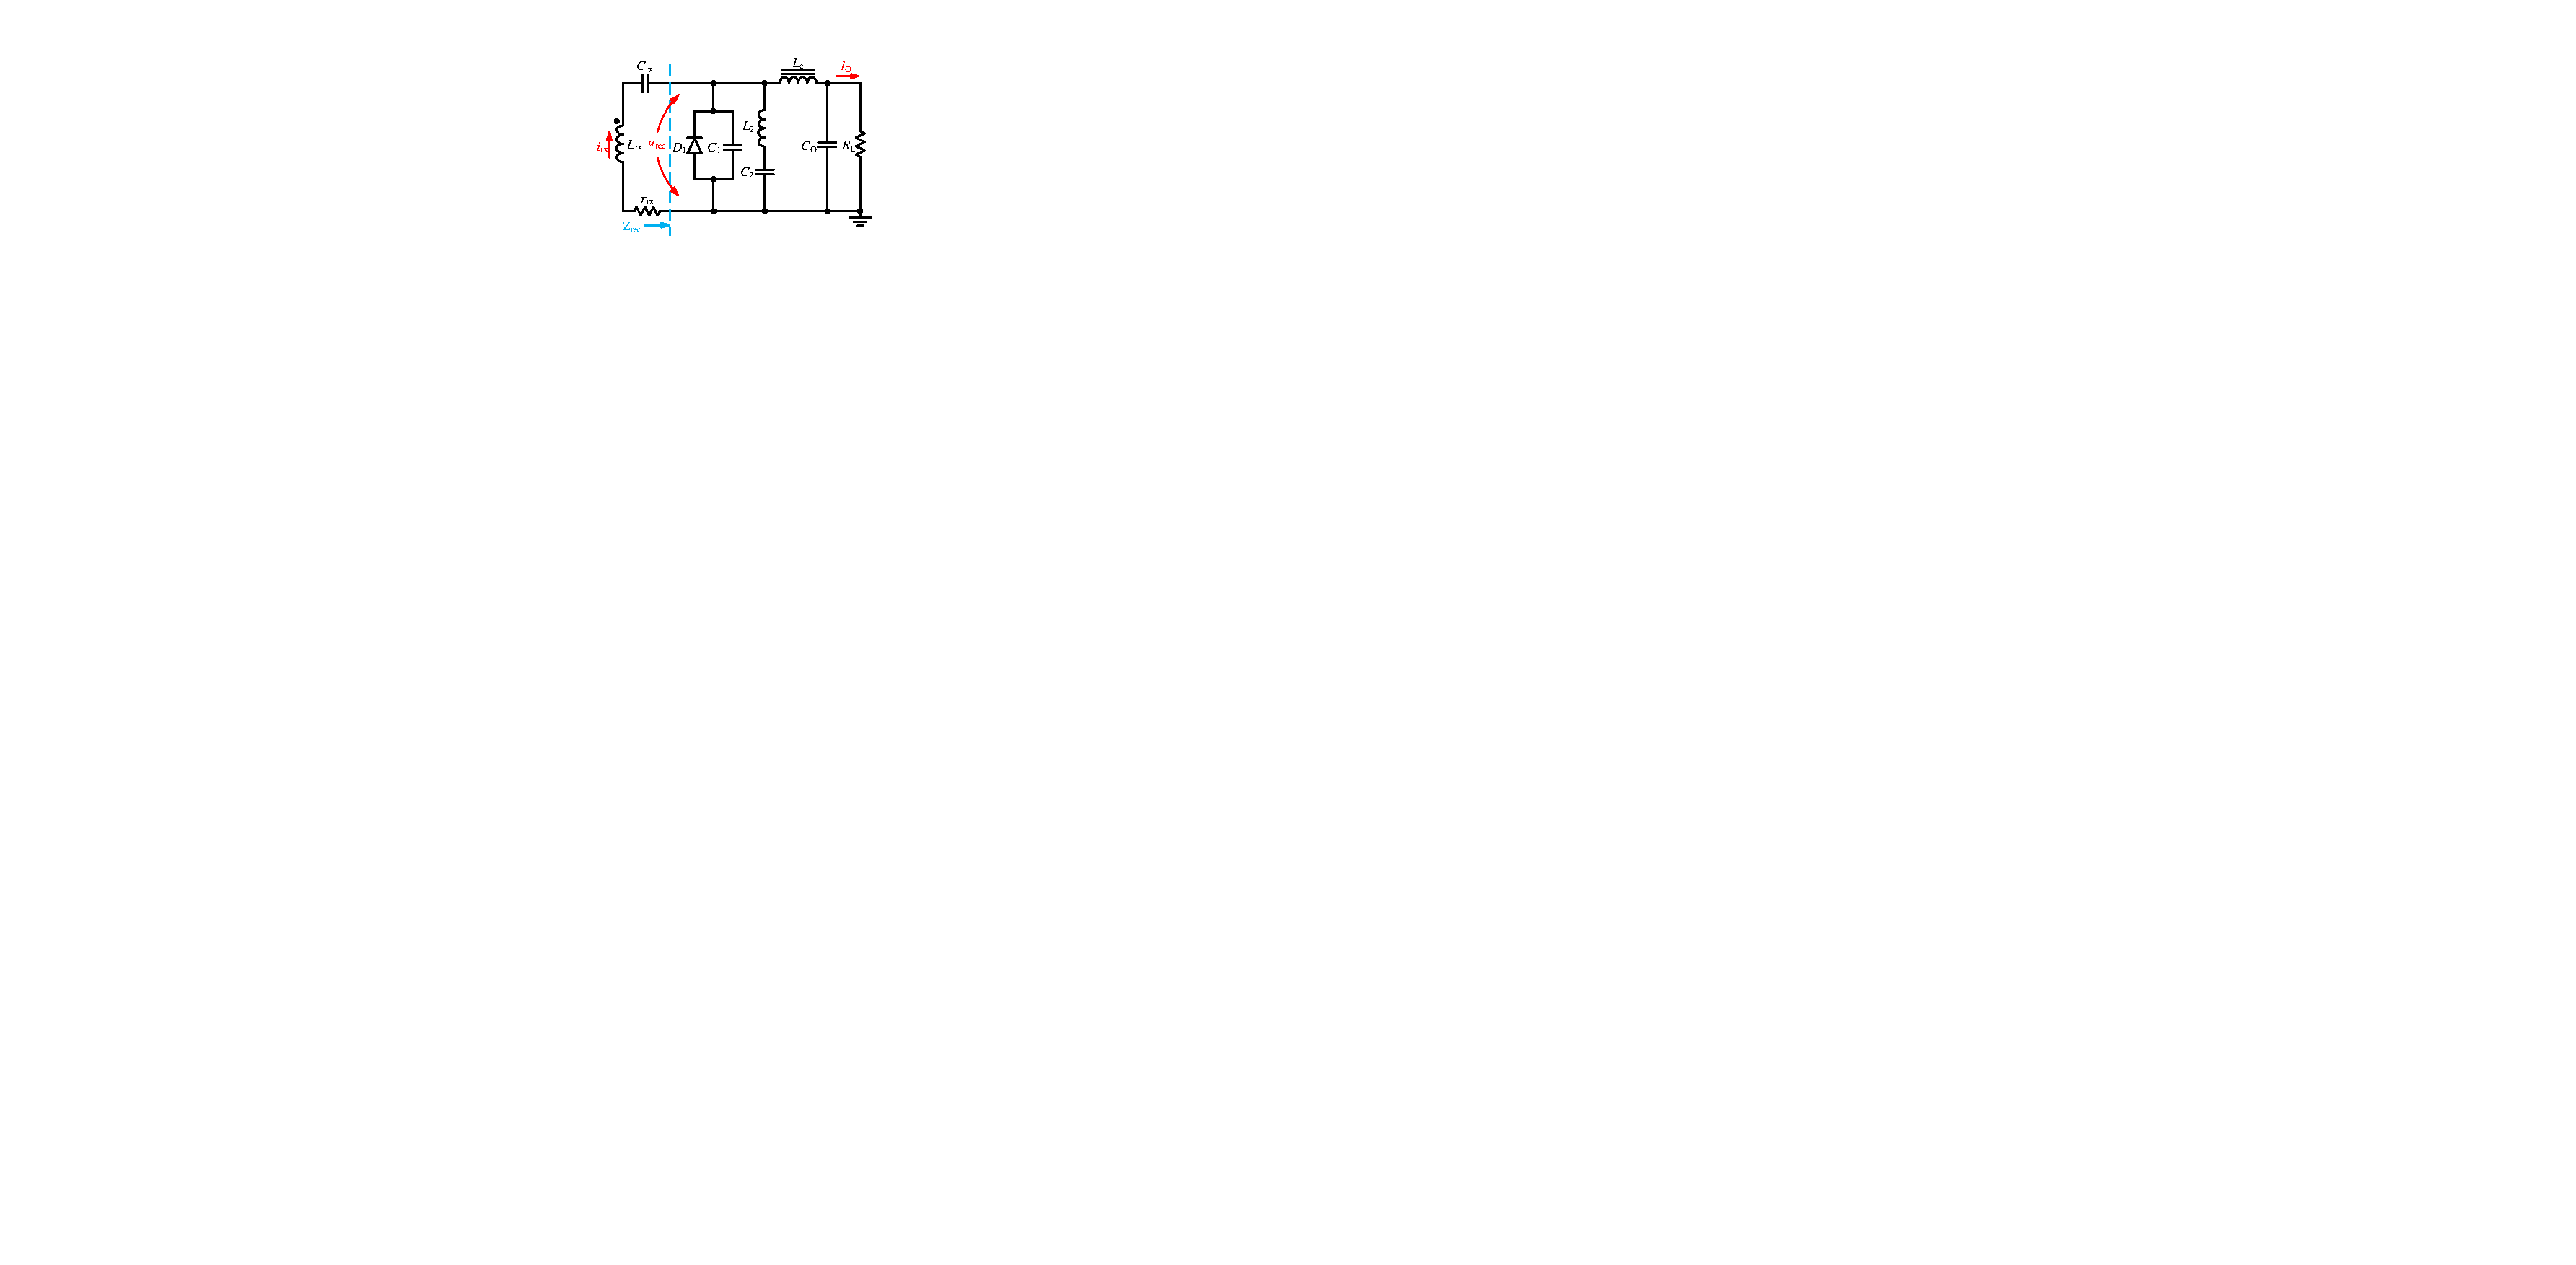
\includegraphics[width=2in]{FiguresEdge/RectifierEF.pdf}}
	\subfigure[]{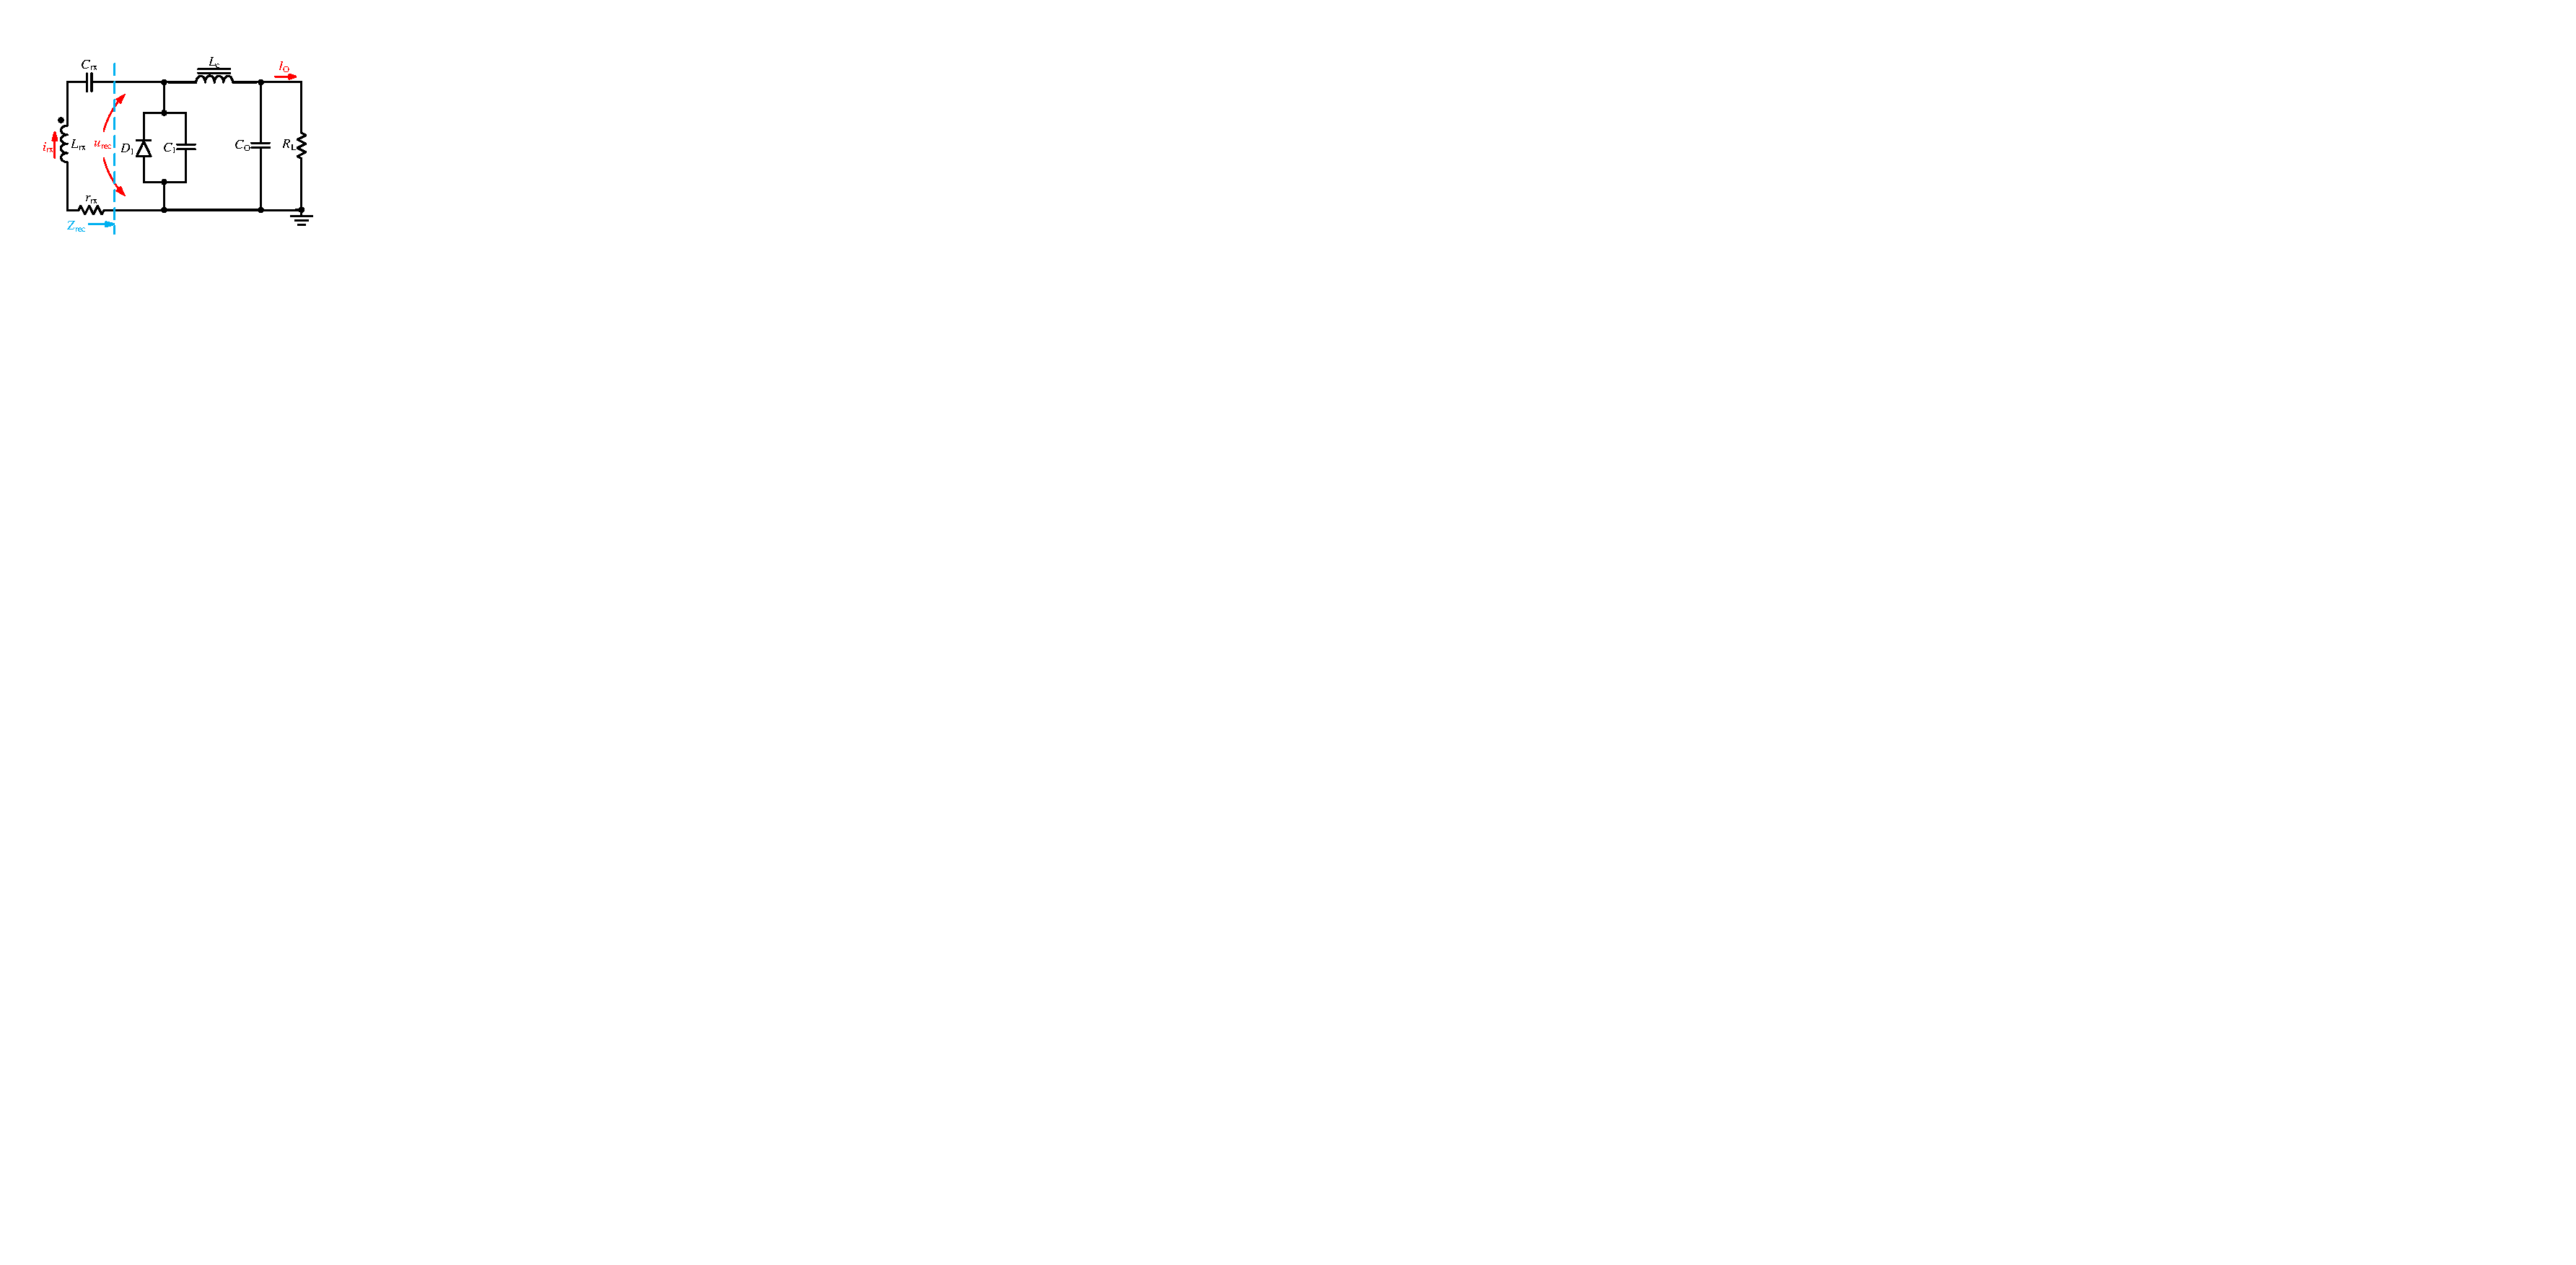
\includegraphics[width=2in]{FiguresEdge/RectifierHalfwave.pdf}}
	\caption{Class E family of rectifiers. (a) Full-wave rectifier. (b) Class EF rectifier. (c) Half-wave rectifier.}
	\label{fig:ClassEfamilyrectifier}
\end{figure}

\ifx\allfiles\undefined
	\onehalfspacing
	\bibliographystyle{chicago}
	%****************************************************************
	%=========This is the file that contains your bibliography entries=======
	%****************************************************************
	\bibliography{HuanBib}
	%=======================================================
	\end{document}
\fi

%\cleardoublepage
%\ifx\allfiles\undefined
	\include{Config} %deifne the using package and the paper layout
	\begin{document}
\else
	
\fi
\chapter{Chapter2 Name}
\section{Overview}
Here is the overview of chapter2. Here is the overview of chapter2. Here is the overview of chapter2. Here is the overview of chapter2

Here is the overview of chapter2. Here is the overview of chapter2. Here is the overview of chapter2. Here is the overview of chapter2

Here is the overview of chapter2. Here is the overview of chapter2. Here is the overview of chapter2. Here is the overview of chapter2

Here is the overview of chapter2. Here is the overview of chapter2. Here is the overview of chapter2. Here is the overview of chapter2

Here is the overview of chapter2. Here is the overview of chapter2. Here is the overview of chapter2. Here is the overview of chapter2

Here is the overview of chapter2. Here is the overview of chapter2. Here is the overview of chapter2. Here is the overview of chapter2

Here is the overview of chapter2. Here is the overview of chapter2. Here is the overview of chapter2. Here is the overview of chapter2

Here is the overview of chapter2. Here is the overview of chapter2. Here is the overview of chapter2. Here is the overview of chapter2
\begin{figure}[!htb]
	\centering
	\subfigure[]{\includegraphics[width=2in]{FiguresEdge/RectifierFullWave.pdf}}
	\subfigure[]{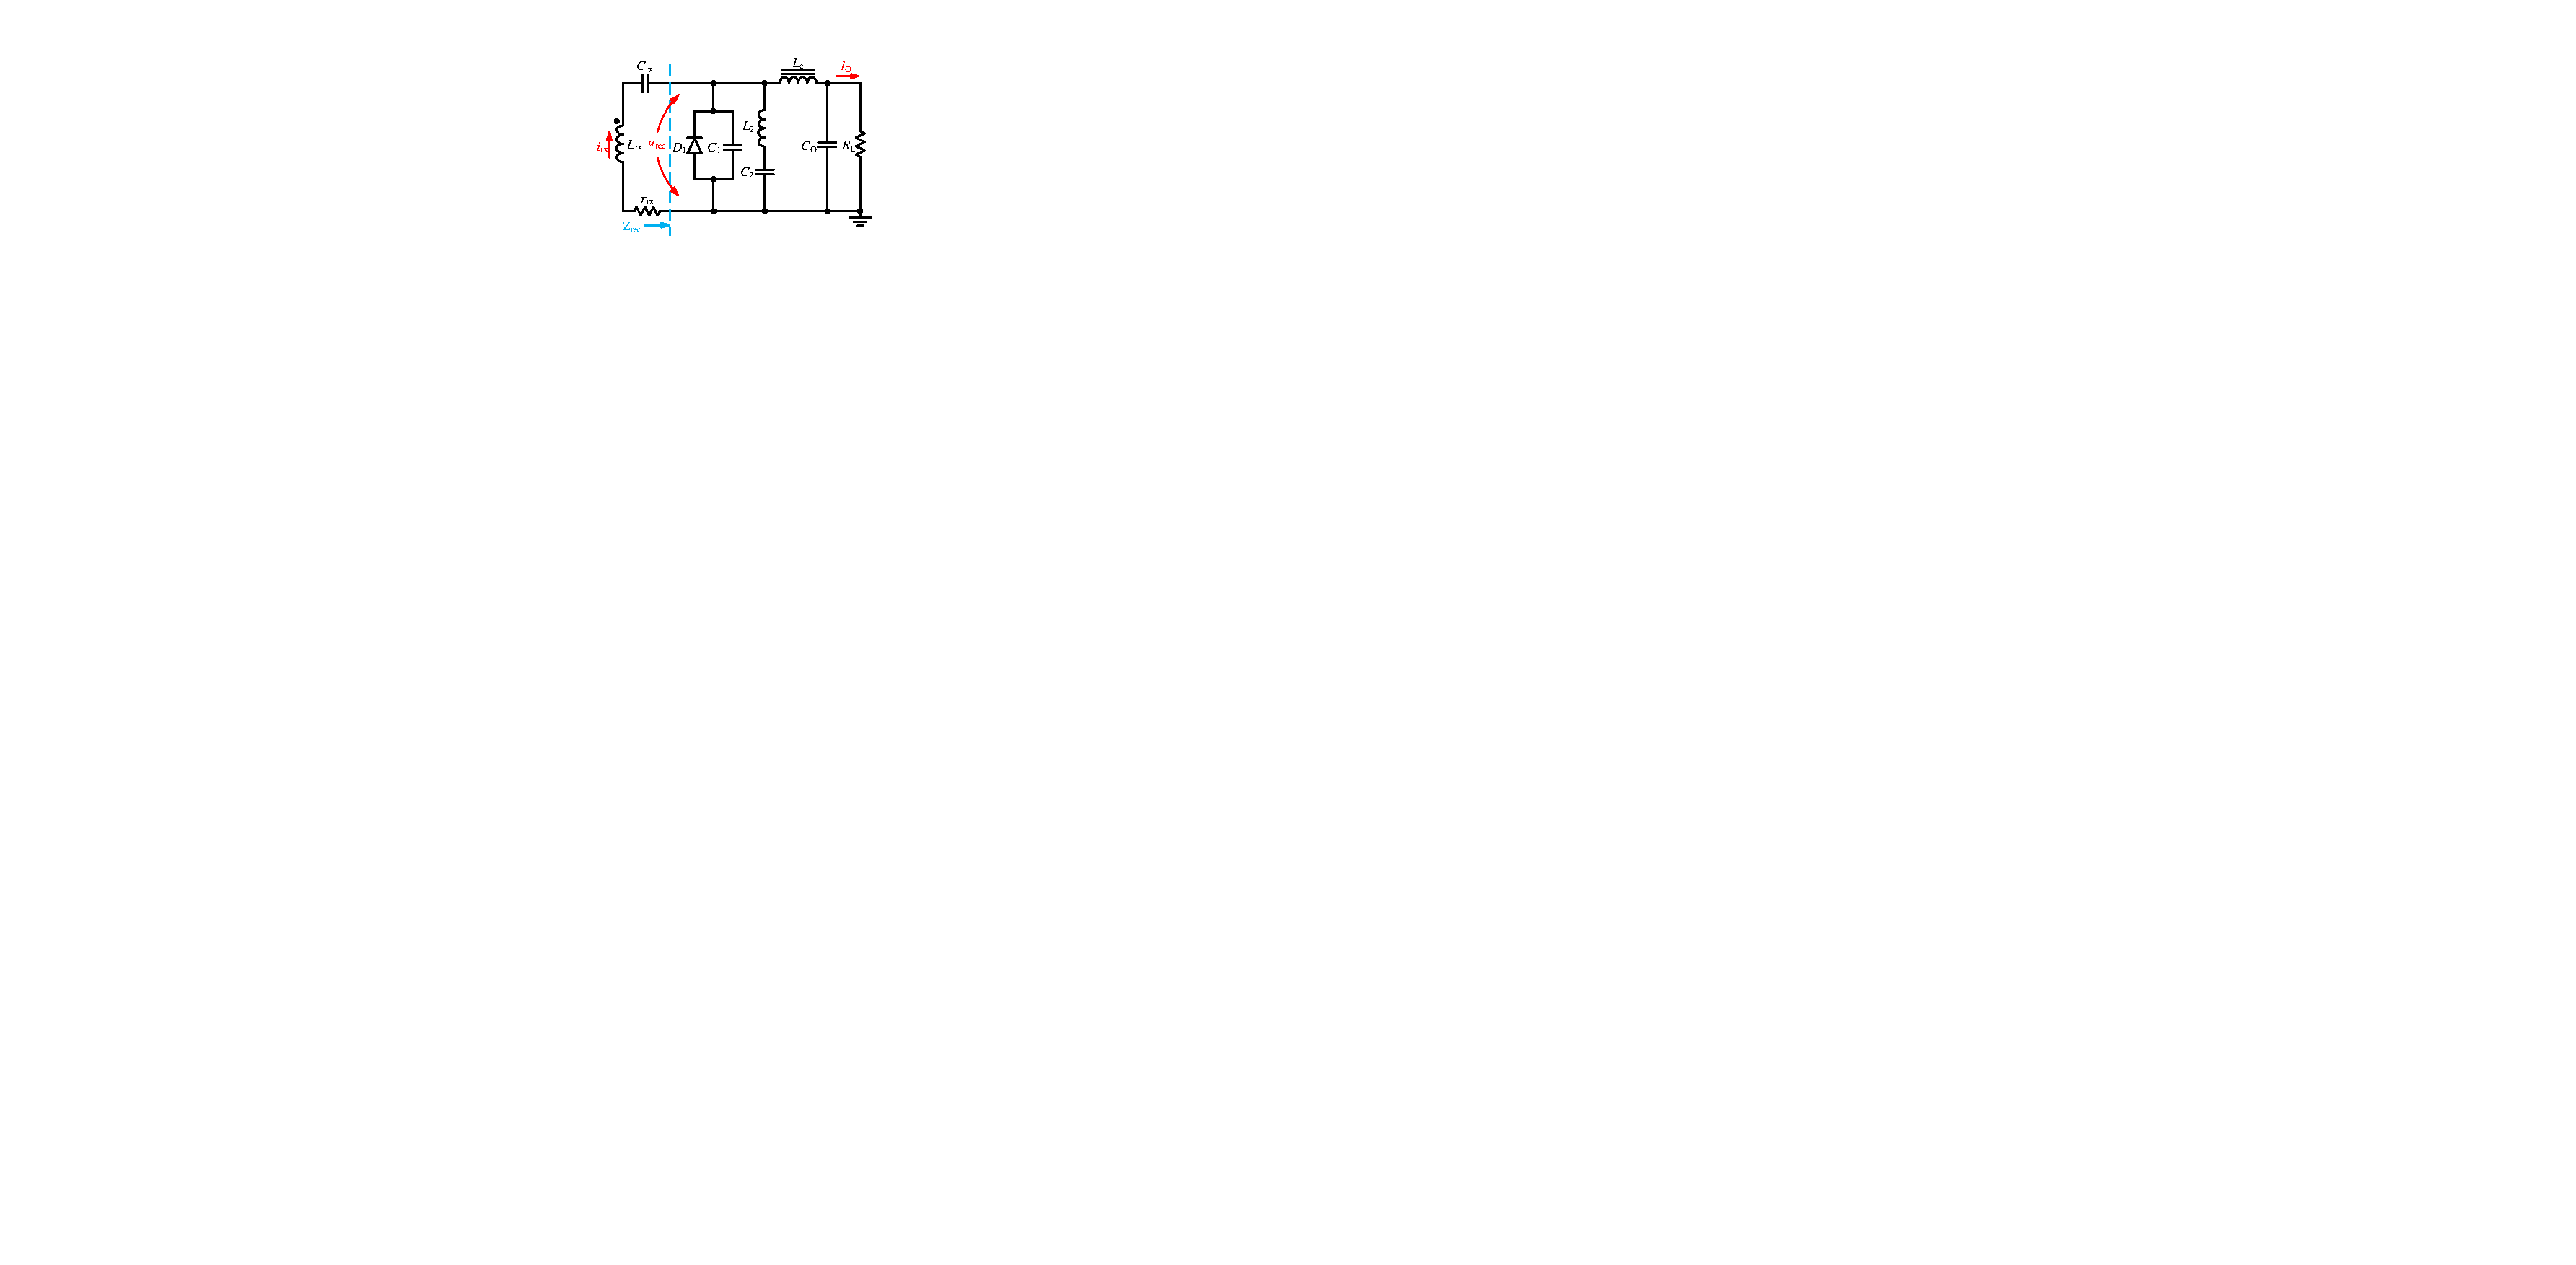
\includegraphics[width=2in]{FiguresEdge/RectifierEF.pdf}}
	\subfigure[]{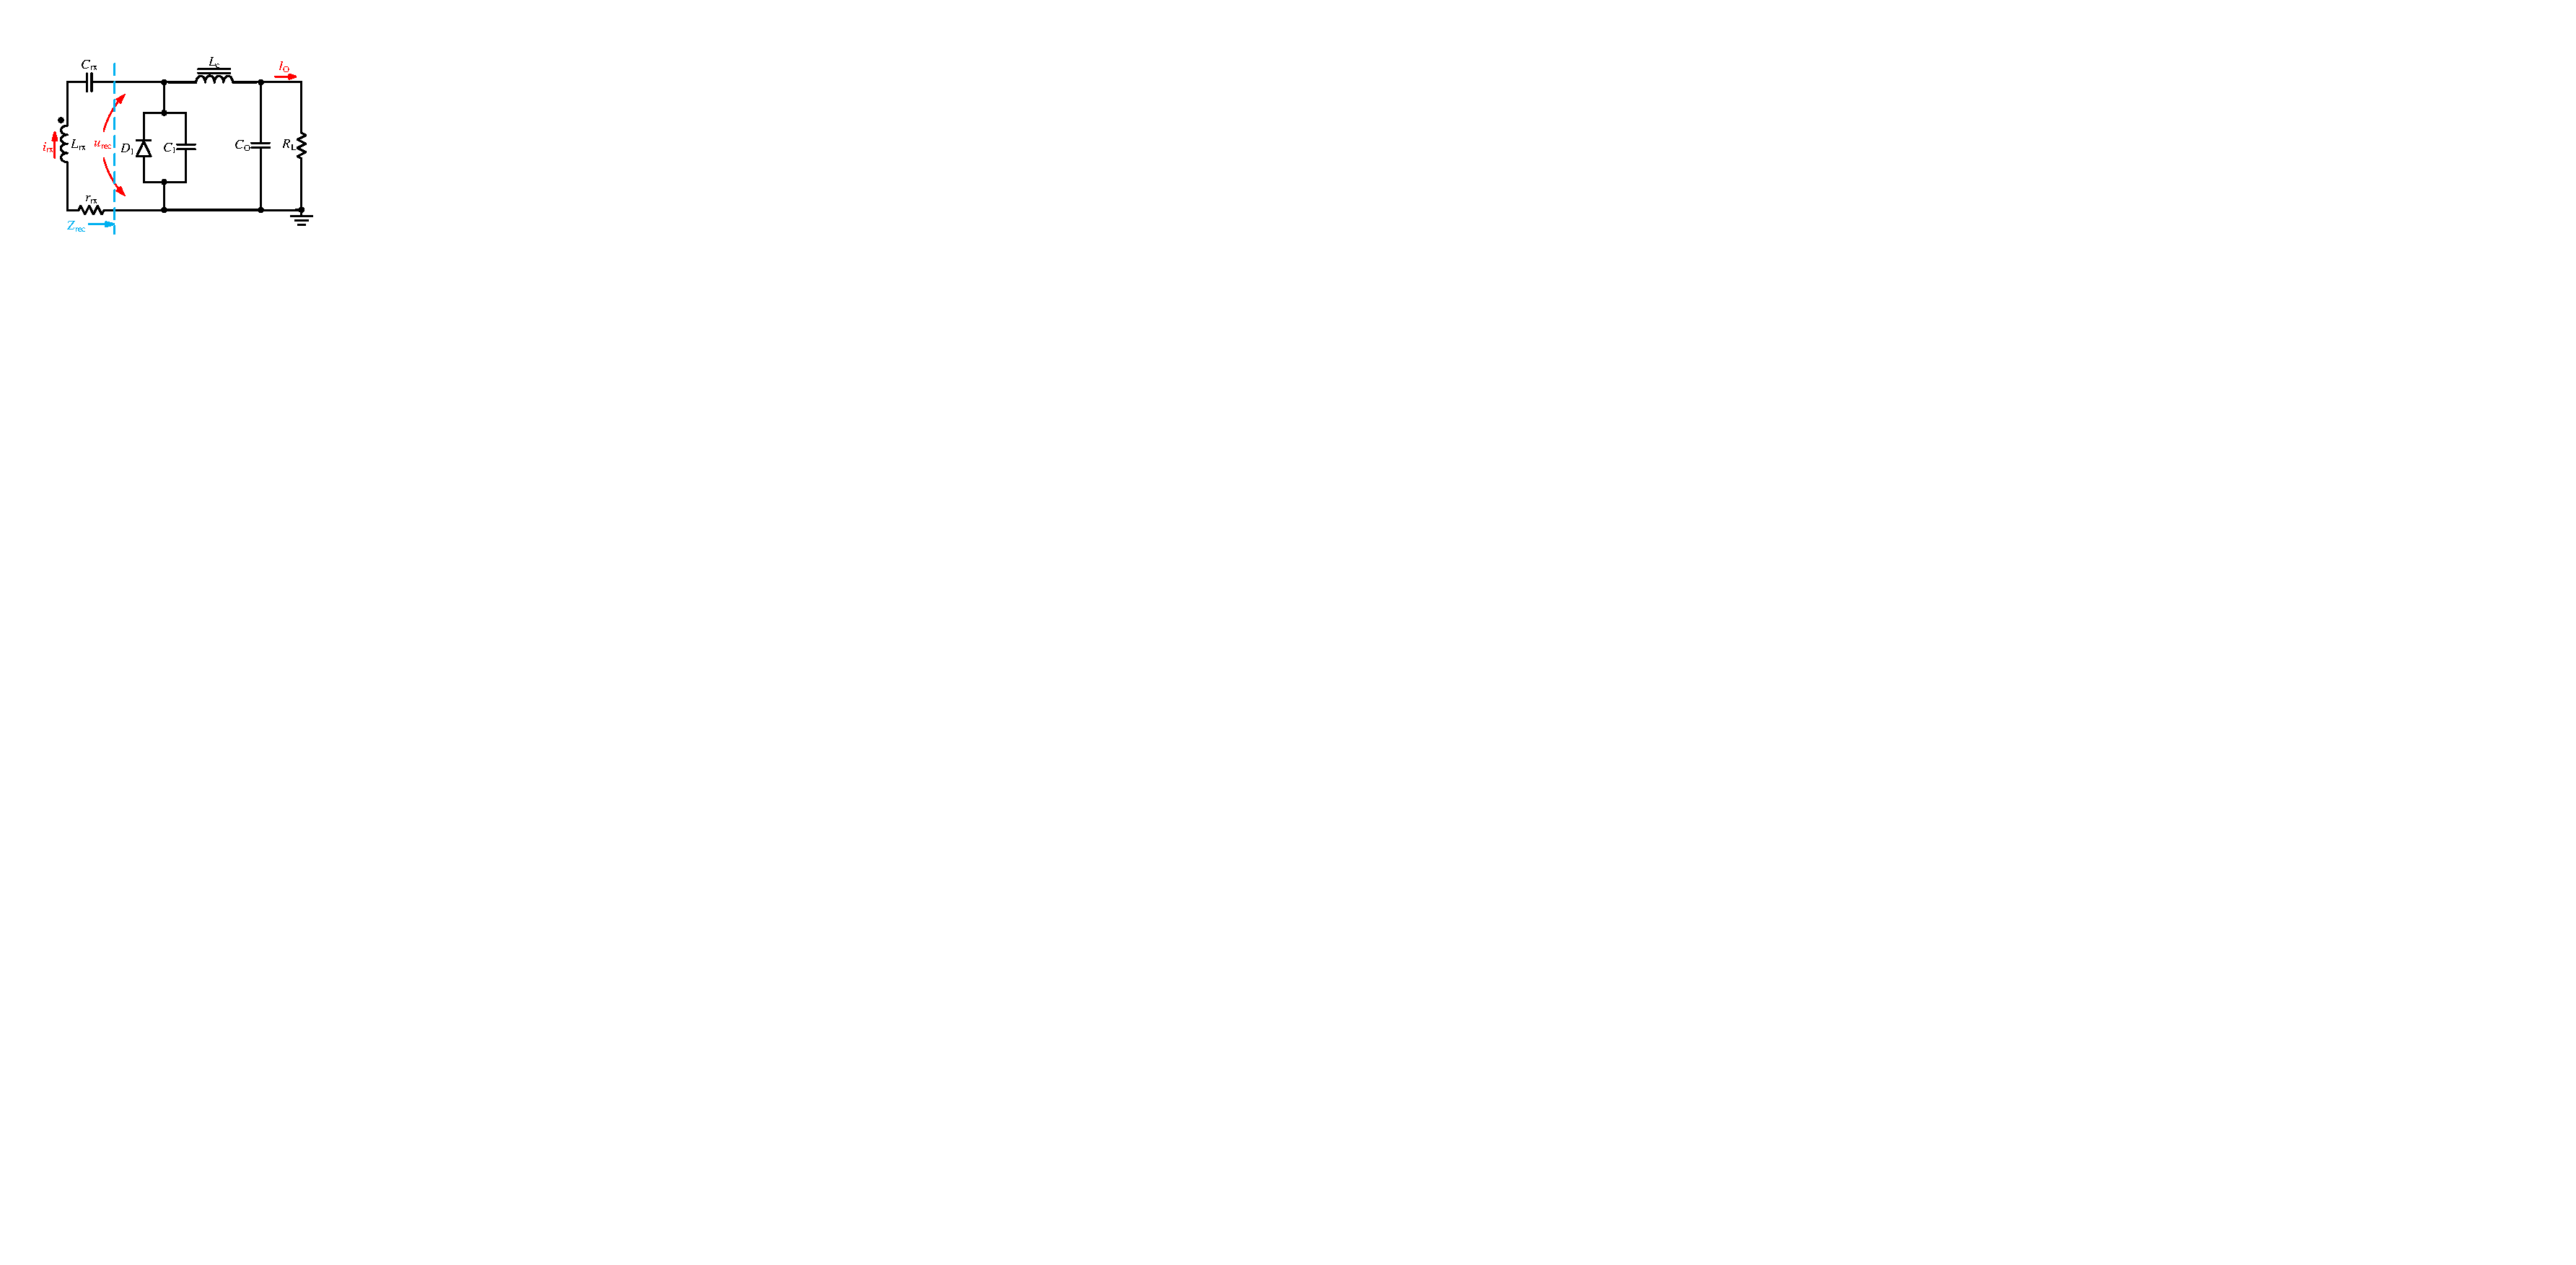
\includegraphics[width=2in]{FiguresEdge/RectifierHalfwave.pdf}}
	\caption{Class E family of rectifiers. (a) Full-wave rectifier. (b) Class EF rectifier. (c) Half-wave rectifier.}
	\label{fig:ClassEfamilyrectifier}
\end{figure}





\ifx\allfiles\undefined
	\onehalfspacing
	\bibliographystyle{chicago}
	%****************************************************************
	%=========This is the file that contains your bibliography entries=======
	%****************************************************************
	\bibliography{HuanBib}
	%=======================================================
	\end{document}
\fi=======================================

%\cleardoublepage
%%\ifx\allfiles\undefined
	\include{Config} %deifne the using package and the paper layout
	\begin{document}
\else
	
\fi
\chapter{Chapter3 Name}
\section{Overview}
Here is the overview of chapter3. Here is the overview of chapter3. Here is the overview of chapter3. Here is the overview of chapter3.

Here is the overview of chapter3. Here is the overview of chapter3. Here is the overview of chapter3. Here is the overview of chapter3.

Here is the overview of chapter3. Here is the overview of chapter3. Here is the overview of chapter3. Here is the overview of chapter3.

Here is the overview of chapter3. Here is the overview of chapter3. Here is the overview of chapter3. Here is the overview of chapter3.

Here is the overview of chapter3. Here is the overview of chapter3. Here is the overview of chapter3. Here is the overview of chapter3.

Here is the overview of chapter3. Here is the overview of chapter3. Here is the overview of chapter3. Here is the overview of chapter3.


\section{Section3}
\label{sec:ModularMRSystem}

\subsection{Modular Architecture}
ABCDE

\ifx\allfiles\undefined
	\onehalfspacing
	\bibliographystyle{chicago}
	%****************************************************************
	%=========This is the file that contains your bibliography entries=======
	%****************************************************************
	\bibliography{HuanBib}
	%=======================================================
	\end{document}
\fi
%%\cleardoublepage
%%\ifx\allfiles\undefined
	\include{Config}
	\begin{document}
\else
	
\fi
\chapter{Current Status and Working Plan}
\section{Overview}
Here is the overview. Here is the overview Here is the overview. Here is the overview. Here is the overview.

Here is the overview. Here is the overview Here is the overview. Here is the overview. Here is the overview

Here is the overview. Here is the overview Here is the overview. Here is the overview. Here is the overview

Here is the overview. Here is the overview Here is the overview. Here is the overview. Here is the overview

Here is the overview. Here is the overview Here is the overview. Here is the overview. Here is the overview

Here is the overview. Here is the overview Here is the overview. Here is the overview. Here is the overview
\section{Summary}\label{sec:Chapter4summary}
Here is the Summary.

\ifx\allfiles\undefined
	\onehalfspacing
	\bibliographystyle{chicago}
	%****************************************************************
	%=========This is the file that contains your bibliography entries=======
	%****************************************************************
	\bibliography{HuanBib}
	%=======================================================
	\end{document}
\fi



%%\cleardoublepage
%%\include{Chapter5}
%%\cleardoublepage
%\include{Conclusion}
%\cleardoublepage
%\chapter*{ACKNOWLEDGEMENT}

Here I would like to thank all the individuals who provide your kind supports and assistances to me and finally make this dissertation possible. It is hard to use words to express my gratitude to all of you.

Foremost, I want to express my heartfelt thanks to my Ph.D supervisor Prof.Chengbin Ma. His wisdom, knowledge, and encouragement really make me to mature as a qualified researcher.
Without his guidance, it is hard for me to make all the accomplishments what I have already achieved. 

Moreover, I would like to express my gratitude to my dissertation committee members, Prof. Houjun Tang, Prof. Jigang Wu, Prof. Mian Li, and Prof. Xinen Zhu. Their detailed guidance and insightful comments are very helpful to further improve the quality of this dissertation and make it more solid, both in terms of technical contents and readability. Also, many thanks to Prof. Patrick Chi-Kwong LUK and Dr. Songnan Yang for their worthful guidance and advice on my research works, especially at the very beginning of my research.

And then, I am grateful to all my lab mates for their selfless helps. I am very enjoy the time working with them all. I also thank the JI staffs for your kind supports throughout my Ph.D program.

Finally, I want to give the special thanks to my family, especially my wife and my son. I will never forget the debt I owe you for your gratuitous support and understanding in the past three years. For this sake, I dedicate the dissertation to you.





%\cleardoublepage
%\include{Appendix}
%\cleardoublepage
%\onehalfspacing
%\bibliographystyle{chicago}
%%****************************************************************
%%=========This is the file that contains your bibliography entries=======
%%****************************************************************
%\bibliography{References}
%%=======================================================
%\end{document}
 %deifne the using package and the paper layout
	\begin{document}
\else
	
\fi
\chapter{Chapter2 Name}
\section{Overview}
Here is the overview of chapter2. Here is the overview of chapter2. Here is the overview of chapter2. Here is the overview of chapter2

Here is the overview of chapter2. Here is the overview of chapter2. Here is the overview of chapter2. Here is the overview of chapter2

Here is the overview of chapter2. Here is the overview of chapter2. Here is the overview of chapter2. Here is the overview of chapter2

Here is the overview of chapter2. Here is the overview of chapter2. Here is the overview of chapter2. Here is the overview of chapter2

Here is the overview of chapter2. Here is the overview of chapter2. Here is the overview of chapter2. Here is the overview of chapter2

Here is the overview of chapter2. Here is the overview of chapter2. Here is the overview of chapter2. Here is the overview of chapter2

Here is the overview of chapter2. Here is the overview of chapter2. Here is the overview of chapter2. Here is the overview of chapter2

Here is the overview of chapter2. Here is the overview of chapter2. Here is the overview of chapter2. Here is the overview of chapter2
\begin{figure}[!htb]
	\centering
	\subfigure[]{\includegraphics[width=2in]{FiguresEdge/RectifierFullWave.pdf}}
	\subfigure[]{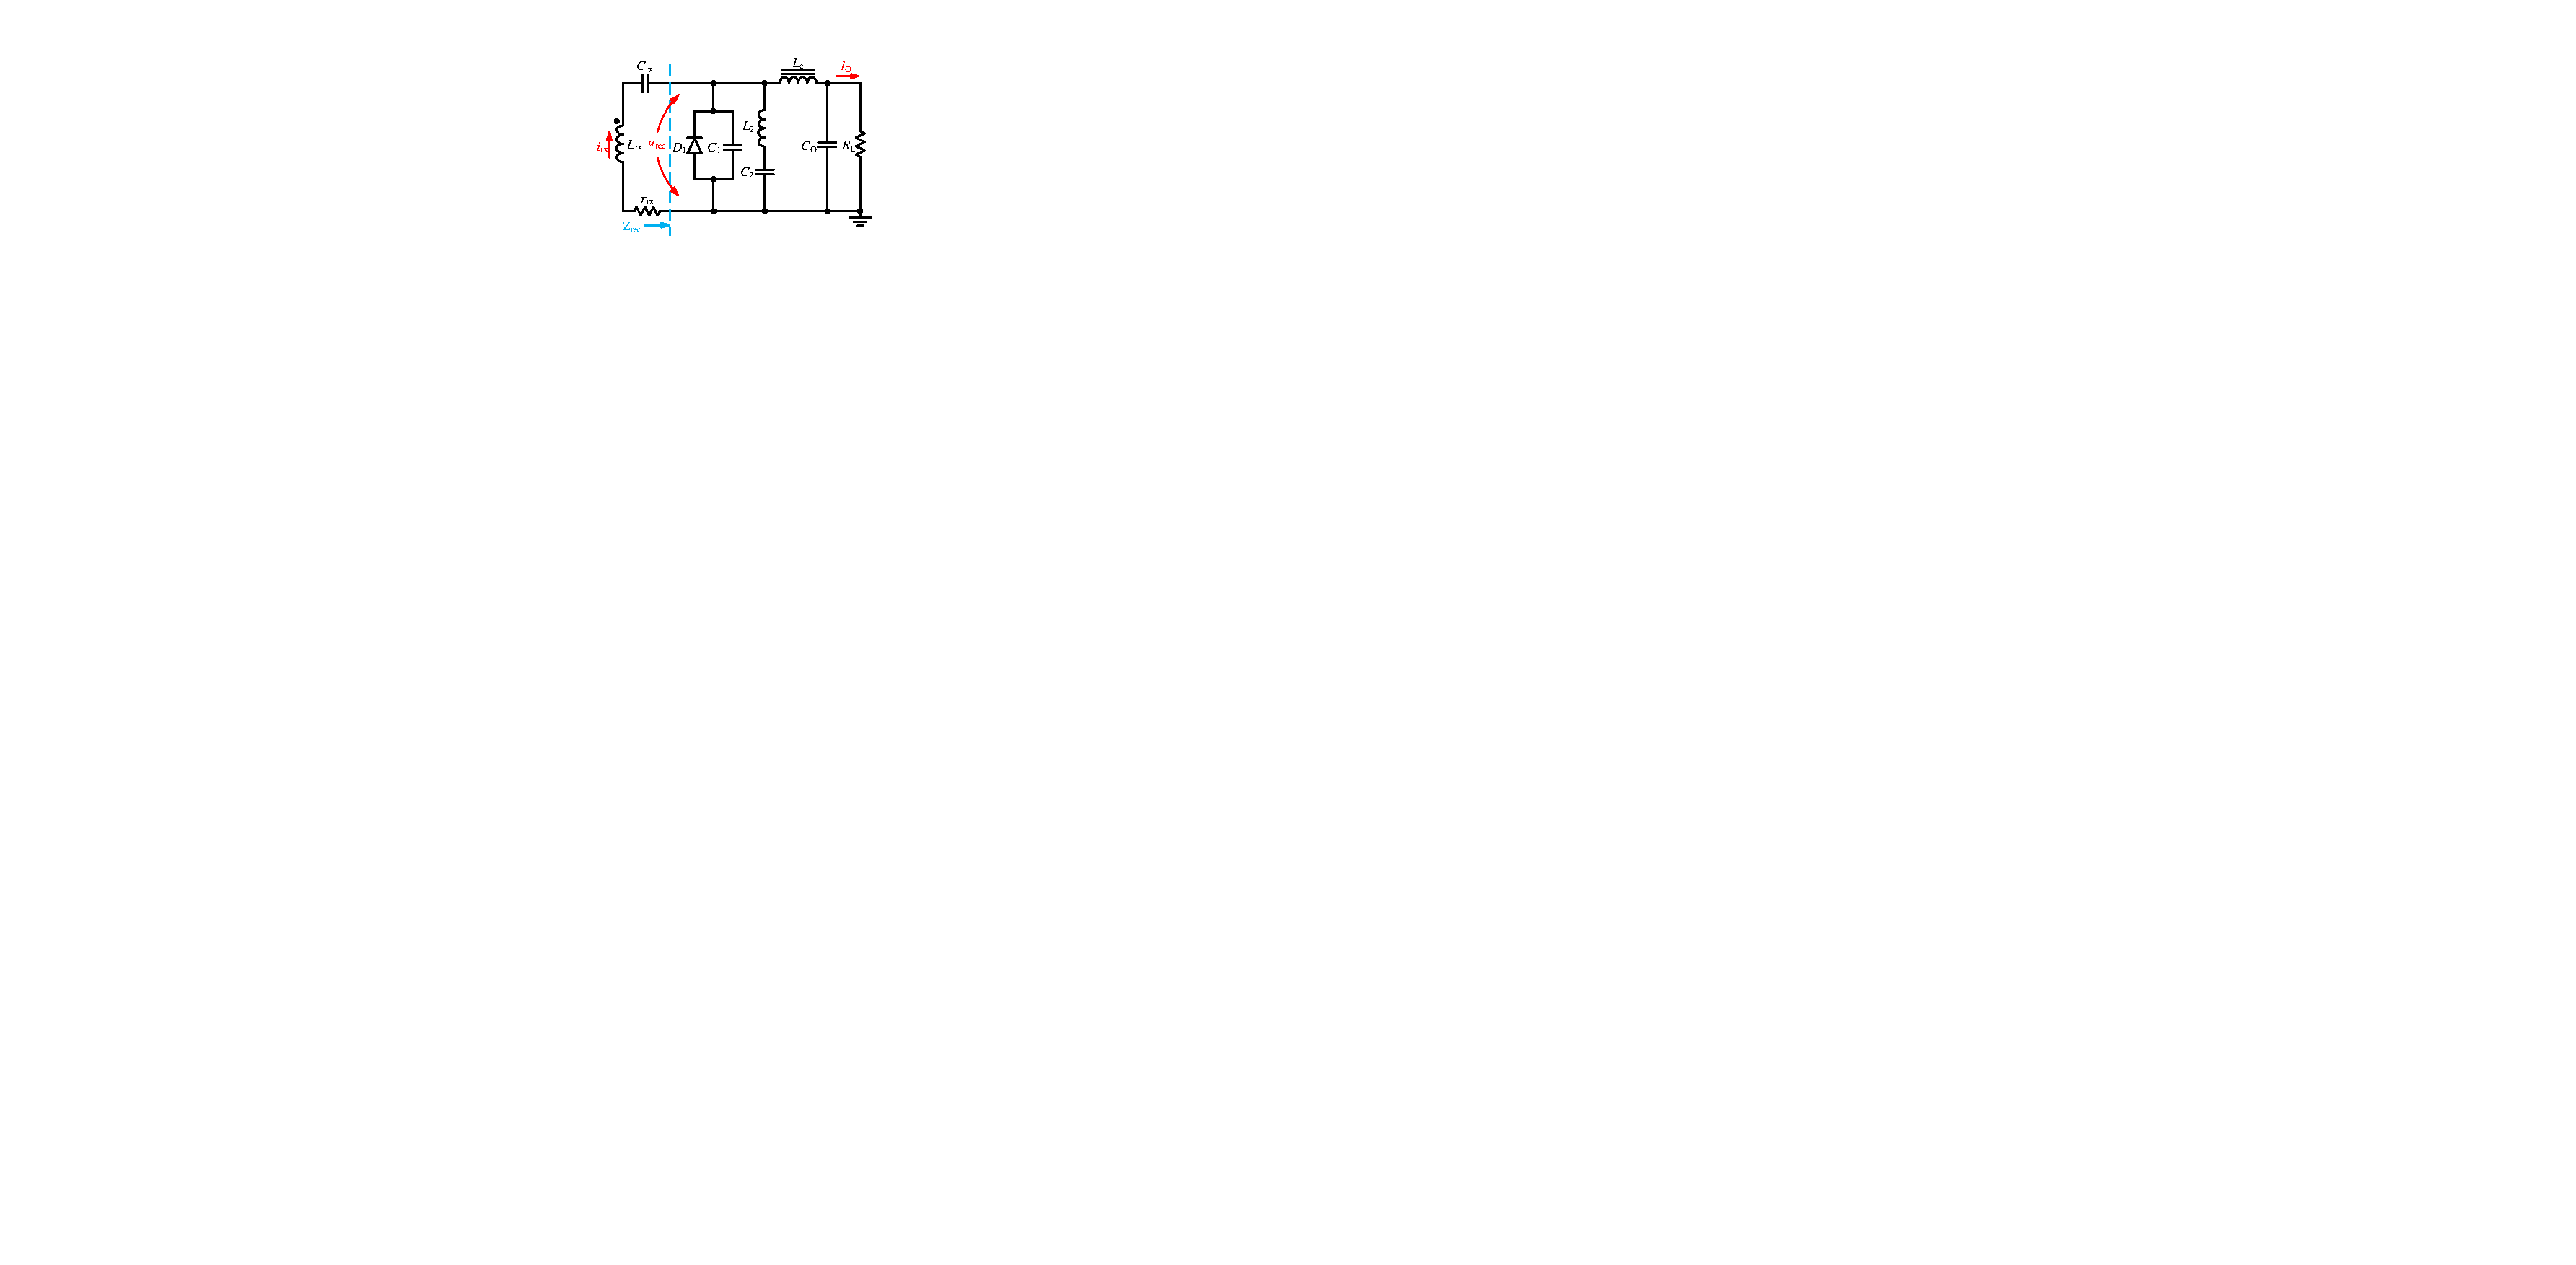
\includegraphics[width=2in]{FiguresEdge/RectifierEF.pdf}}
	\subfigure[]{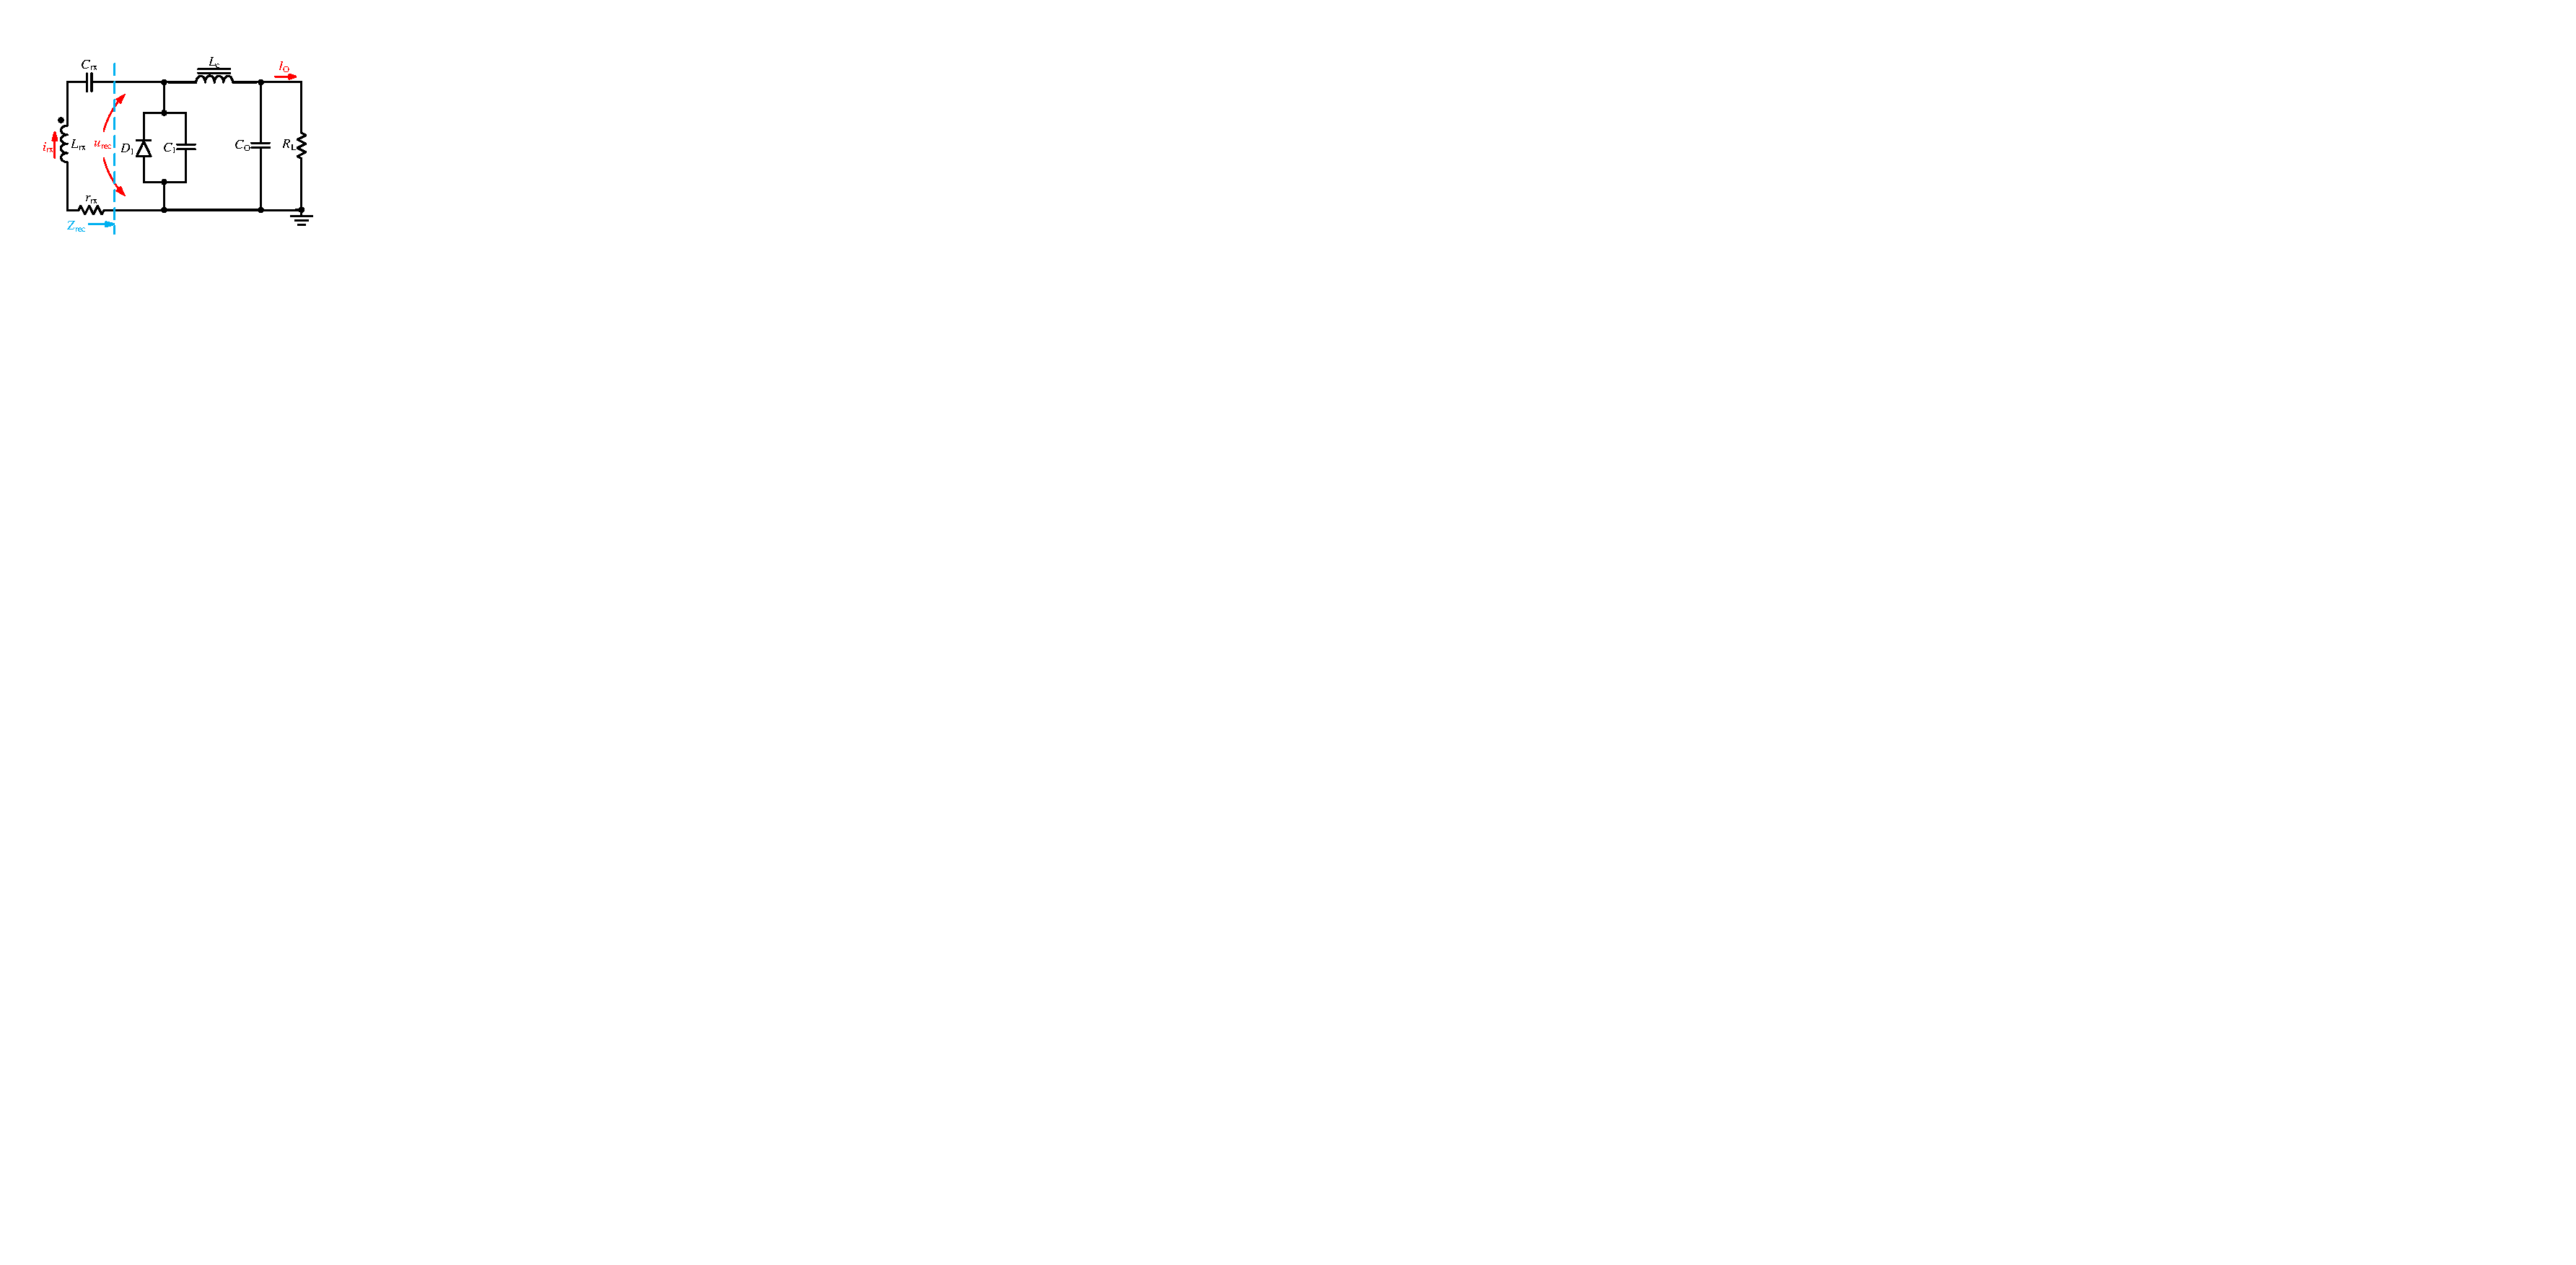
\includegraphics[width=2in]{FiguresEdge/RectifierHalfwave.pdf}}
	\caption{Class E family of rectifiers. (a) Full-wave rectifier. (b) Class EF rectifier. (c) Half-wave rectifier.}
	\label{fig:ClassEfamilyrectifier}
\end{figure}





\ifx\allfiles\undefined
	\onehalfspacing
	\bibliographystyle{chicago}
	%****************************************************************
	%=========This is the file that contains your bibliography entries=======
	%****************************************************************
	\bibliography{HuanBib}
	%=======================================================
	\end{document}
\fi=======================================

%\cleardoublepage
%%\ifx\allfiles\undefined
	\documentclass[12pt,a4paper,twoside,openright]{report}
%
%-----Packages
%
\usepackage[english]{babel}
\usepackage{setspace}
\usepackage[T1]{fontenc}
\usepackage[latin1]{inputenc}
\usepackage[intlimits]{amsmath}
\usepackage{amsfonts,amssymb}
\usepackage{natbib}
\usepackage[normalsize,bf]{caption}
\usepackage[dvips]{graphicx}
\usepackage{color}
\usepackage[breaklinks,linktocpage]{hyperref}
\usepackage{fancyhdr}
\usepackage{setspace}
\usepackage{subfigure}
\usepackage{float}
\usepackage{lettrine}
\usepackage{comment}
\usepackage{pifont}
\usepackage{soul, color}  %\hl
\usepackage{booktabs}	  %\toprule in table
\usepackage{tabularx}	  %\tabular
\usepackage{multicol}	  %table col
\usepackage{multirow}	  %table row
\usepackage{diagbox}

\newcommand{\hlg}[2][green]{{\sethlcolor{#1}\hl{#2}}}
\newcommand{\tabincell}[2]{\begin{tabular}{@{}#1@{}}#2\end{tabular}}
\sloppy\par
%****************************************************************
% ===========Optional packages (uncomment as needed)=============
%****************************************************************
\usepackage{wrapfig}
%\usepackage{makeidx}
\usepackage{amsbsy}
\usepackage{latexsym}
\usepackage{amsthm}
\usepackage{datatool}
%\usepackage{glossary}
\usepackage{glossaries}
%\makeglossary
%\makeglossaries


%=======================================================
%
%-----Layout
%
\onehalfspacing
\hoffset = -1 in
\voffset= -1 in
%
%-----Set margins for a4 paper
%
\topmargin = 3.0cm
\textwidth = 17cm
\textheight = 22cm
\oddsidemargin =  2cm
\evensidemargin = 2cm
%
%-----Headers and Footers
%
\pagestyle{fancyplain}
\renewcommand{\chaptermark}[1]%
{\markboth{#1}{}}
\renewcommand{\sectionmark}[1]%
{\markright{\thesection\ -- #1}}
\lhead[\fancyplain{}{\thepage}]%
{\fancyplain{}{\rightmark}}
\rhead[\fancyplain{}{\leftmark}]%
{\fancyplain{}{\thepage}}
\cfoot{}
%
%-----No headers on empty pages before new chapter
%
\makeatletter
\def\cleardoublepage{\clearpage\if@twoside \ifodd\c@page\else
	\hbox{}
	\thispagestyle{plain}
	\newpage
	\if@twocolumn\hbox{}\newpage\fi\fi\fi}
\makeatother \clearpage{\pagestyle{plain}\cleardoublepage}
%
%-----Footnotes
%
\renewcommand{\thefootnote}{\fnsymbol{footnote}} % Footnotes are marked with symbols instead of literals
\setlength{\textfloatsep}{8pt plus 4pt minus 4pt}        % Separation of floats from text
\renewcommand{\bibnumfmt}[1]{{\scriptsize #1}}
\setlength{\bibhang}{2em}
%
%-----Define Horizontal rule
%
\newcommand{\HRule}{\rule{\textwidth}{0.5mm}}
%
%-----Define Hyperlink colors
%
\definecolor{darkred}{rgb}{0.25,0,0}
\definecolor{darkgreen}{rgb}{0,0.25,0}
\definecolor{darkblue}{rgb}{0,0,0.5}
\hypersetup{colorlinks,linkcolor=black,filecolor=black,urlcolor=darkblue,citecolor=black}
\usepackage{breakurl}
%****************************************************************
% ===========Add user definitions as needed=====================
%****************************************************************
%\include{definitions}
\newtheorem{theorem}{Theorem}[chapter]
\newtheorem{principle}{Principle}[chapter]
\newtheorem{algorithm}{Algorithm}[chapter]
\newtheorem{law}{Law}
%\theoremstyle{plain}  % Default
\theoremstyle{definition}
%\theoremstyle{remark}
\newtheorem{problem}{Problem}[chapter]
\newtheorem{example}{Example}[chapter]
\newtheorem{definition}{Definition}[chapter]




%%***********Config file orginal backup*********
%\immediate\write18{makeindex \jobname.nlo -s nomencl.ist -o \jobname.nls}
%\documentclass[12pt,a4paper,twoside,openright]{report}
%%
%%-----Packages
%%
%\usepackage[english]{babel}
%\usepackage{setspace}
%\usepackage[T1]{fontenc}
%\usepackage[latin1]{inputenc}
%\usepackage[intlimits]{amsmath}
%\usepackage{amsfonts,amssymb}
%\usepackage{natbib}
%\usepackage[normalsize,bf]{caption}
%\usepackage[dvips]{graphicx}
%%\usepackage{color}
%%\usepackage{mathdots}
%%\usepackage{mathtools}
%%\usepackage{booktabs}
%%\usepackage{multirow}
%%\usepackage{ps2pdf}
%\usepackage{epstopdf}
%\usepackage[breaklinks,linktocpage]{hyperref}
%\usepackage{fancyhdr}
%\usepackage{setspace}
%\usepackage{subfigure}
%\usepackage{lettrine}
%\newcommand{\tabincell}[2]{\begin{tabular}{@{}#1@{}}#2\end{tabular}}
%\sloppy\par
%%****************************************************************
%% ===========Optional packages (uncomment as needed)=============
%%****************************************************************
%\usepackage{wrapfig}
%%\usepackage{makeidx}
%\usepackage{amsbsy}
%\usepackage{latexsym}
%\usepackage{amsthm}
%\usepackage{datatool}
%\usepackage{nomencl}
%\makenomenclature
%\usepackage{glossaries}
%\makeglossaries
%\usepackage{ifthen}
%\usepackage{graphicx}
%\usepackage{color, soul}
%%\usepackage{wasysym}
%%\usepackage{psfrag}
%%\usepackage{subfig}
%%\usepackage{pifont}
%%\usepackage{longtable}
%%\setlength\LTleft{0pt}
%%\setlength\LTright{0pt}
%%=======================================================
%%
%%-----Layout
%%
%\onehalfspacing
%\hoffset = -1 in
%\voffset= -1 in
%%
%%-----Set margins for a4 paper
%%
%\topmargin = 3.0cm
%\textwidth = 17cm
%\textheight = 22cm
%\oddsidemargin =  2cm
%\evensidemargin = 2cm
%%
%%-----Headers and Footers
%%
%\pagestyle{fancyplain}
%\renewcommand{\chaptermark}[1]%
%            {\markboth{#1}{}}
%\renewcommand{\sectionmark}[1]%
%            {\markright{\thesection\ -- #1}}
%\lhead[\fancyplain{}{\thepage}]%
%      {\fancyplain{}{\rightmark}}
%\rhead[\fancyplain{}{\leftmark}]%
%     {\fancyplain{}{\thepage}}
%\cfoot{}
%%
%%-----No headers on empty pages before new chapter
%%
%\makeatletter
%\def\cleardoublepage{\clearpage\if@twoside \ifodd\c@page\else
%    \hbox{}
%    \thispagestyle{plain}
%    \newpage
%    \if@twocolumn\hbox{}\newpage\fi\fi\fi}
%\makeatother \clearpage{\pagestyle{plain}\cleardoublepage}
%%
%%-----Footnotes
%%
%\renewcommand{\thefootnote}{\fnsymbol{footnote}} % Footnotes are marked with symbols instead of literals
%\setlength{\textfloatsep}{8pt plus 4pt minus 4pt}        % Separation of floats from text
%\renewcommand{\bibnumfmt}[1]{{\scriptsize #1}}
%\setlength{\bibhang}{2em}
%%
%%-----Define Horizontal rule
%%
%\newcommand{\HRule}{\rule{\textwidth}{0.5mm}}
%%
%%-----Define Hyperlink colors
%%
%\definecolor{darkred}{rgb}{0.25,0,0}
%\definecolor{darkgreen}{rgb}{0,0.25,0}
%\definecolor{darkblue}{rgb}{0,0,0.5}
%\hypersetup{colorlinks,linkcolor=black,filecolor=black,urlcolor=darkblue,citecolor=black}
%\usepackage{breakurl}
%
%%****************************************************************
%% ===========Add user definitions as needed=====================
%%****************************************************************
%\include{definitions}
%\newtheorem{theorem}{Theorem}[chapter]
%\newtheorem{principle}{Principle}[chapter]
%%\newtheorem{algorithm}{Algorithm}[chapter]
%\newtheorem{law}{Law}
%%\theoremstyle{plain}  % Default
%\theoremstyle{definition}
%%\theoremstyle{remark}
%\newtheorem{problem}{Problem}[chapter]
%\newtheorem{example}{Example}[chapter]
%\newtheorem{definition}{Definition}[chapter]
%%=======================================================
%%%%%%%%%%%%%
%%-----Begin Document
%%%%%%%%%%%%%
%\begin{document}
%\pagenumbering{roman}
%%
%%-----Title page
%%
%
%\begin{titlepage}
%\noindent {\bf Shanghai Jiao Tong University \\
%University of Michigan- Shanghai Jiao Tong University Joint Institute}\\
%\noindent \HRule \vspace{0.0455\textheight}
%%****************************************************************
%% ===========Edit the following lines to get the right title============
%%****************************************************************
%\begin{center}
%{\huge \bf Proposal Name}\\[0.016\textheight]
%{\Large \bf Doctoral Dissertation Proposal} \\[0.032\textheight]
%\large{by} \\[0.032\textheight] \Large{ \bf Jibin Song}\\
%%=======================================================
%\vspace{5cm}
%\normalsize{A proposal submitted in satisfaction of the \\
%requirements for the degree of Doctor of Philosophy in \\
%Control Science and Engineering at Shanghai Jiao Tong University}
%\HRule \\[0.023\textheight]
%%****************************************************************
%%======Edit the following lines to get the right committee members======
%%****************************************************************
%\begin{tabular*}{\textwidth}{@{}l@{\extracolsep{\fill}}r@{}}
%\textbf{Committee in charge:} &  \textbf{Shanghai}\\
%\textbf{Professor XXX} &  \textbf{July, 2020}\\
%\textbf{Professor XXX} & \\
%\textbf{Professor XXX} & \\
%\textbf{Professor XXX} & \\
%\textbf{Professor XXX} & \\
%\end{tabular*}
%%=======================================================
%\end{center}
%\end{titlepage}
%
%%
%%-----Abstract
%%
%\thispagestyle{empty}
%\cleardoublepage
%%****************************************************************
%%===========Your abstract goes in the file Abstract.tex==============
%%****************************************************************
%
%
%
%\begin{abstract}
\noindent

Here is the abstract. Here is the abstract. Here is the abstract. Here is the abstract.

Here is the abstract. Here is the abstract. Here is the abstract. Here is the abstract.

Here is the abstract. Here is the abstract. Here is the abstract. Here is the abstract.

Here is the abstract. Here is the abstract. Here is the abstract. Here is the abstract.

Here is the abstract. Here is the abstract. Here is the abstract. Here is the abstract.

Here is the abstract. Here is the abstract. Here is the abstract. Here is the abstract.

Here is the abstract. Here is the abstract. Here is the abstract. Here is the abstract.

Here is the abstract. Here is the abstract. Here is the abstract. Here is the abstract.
\end{abstract}



%\cleardoublepage
%\newlength{\nomitemorigsep}
\setlength{\nomitemorigsep}{\nomitemsep}
\setlength{\nomitemsep}{-\parsep}
\makenomenclature
\renewcommand{\nomgroup}[1]{%
  \itemsep\nomitemorigsep%
  \ifthenelse{%
    \equal{#1}{A}%
  }{%
  \item[\textbf{Abbreviations}]%

  }{%
    \ifthenelse{\equal{#1}{S}}{%
    \item[\textbf{List of Symbols}]%

    }{}%
  }%
  \itemsep\nomitemsep
}
\renewcommand{\nomname}{Nomenclature}
\markboth{\MakeUppercase\nomname}{\MakeUppercase\nomname}
\printnomenclature[0.8in]
\nomenclature[A]{ADS}{Advanced Design System}
\nomenclature[A]{ESR}{Equivalent series resistance}
\nomenclature[A]{MOSFET}{Metal-oxide-semiconductor field effect transistor}
\nomenclature[A]{MWPT}{Multiple-receiver wrieless power transfer}
\nomenclature[A]{PA}{Power amplifier}
\nomenclature[A]{RF}{Radio frequency}
\nomenclature[A]{SRR}{Synchronous Resonant Rectifier}
\nomenclature[A]{WPT}{Wireless power transfer}
\nomenclature[A]{ZVS}{Zero-voltage-switching}




\nomenclature[S]{$C_{0}$}{Capacitor in resonant tank of Class E PA}
\nomenclature[S]{$C_{r}$}{Diode/switch shunt capacitor of Class E rectifier}
\nomenclature[S]{$C_{S}$}{Switch shunt capacitor of Class E PA}
\nomenclature[S]{$C_{rx}$}{Compensation capacitor of receiving coil}
\nomenclature[S]{$C_{tx}$}{Compensation capacitor of transmitting coil}
\nomenclature[S]{$k$}{Mutual inductance coefficient of coupling coils}
\nomenclature[S]{$k_{ij}$}{Mutual inductance coefficient between $i$-th and $j$-th coils in MWPT}
\nomenclature[S]{$L_{0}$}{Inductor in resonant tank of Class E PA}
\nomenclature[S]{$L_{rx}$}{Inductance of receiving coil}
\nomenclature[S]{$L_{tx}$}{Inductance of transmitting coil}
\nomenclature[S]{$M$}{Mutual inductance of coupling coils}
\nomenclature[S]{$M_{ij}$}{Mutual inductance between $i$-th and $j$-th coils in MWPT}
\nomenclature[S]{$r_{rx}$}{ESR of receiving coil}
\nomenclature[S]{$r_{tx}$}{ESR of transmitting coil}
\nomenclature[S]{$R_{L}$}{Dc load of rectifier}
\nomenclature[S]{$R_{rec}$}{Input resisance of rectifier}
\nomenclature[S]{$v_{DS}$}{Drain-source voltage of MOSFET}
\nomenclature[S]{$v_{GS}$}{Gate-source voltage of MOSFET}
\nomenclature[S]{$X_{rec}$}{Input reactance of rectifier}
\nomenclature[S]{$Z_{rec}$}{Input impedance of rectifier}
\nomenclature[S]{$Z_{coil}$}{Input impedance of transmitting coil}
\nomenclature[S]{$\eta_{PA}$}{Efficiency of PA}
\nomenclature[S]{$\eta_{rec}$}{Efficiency of rectifier}
\nomenclature[S]{$\eta_{sys}$}{Dc-dc efficiency of WPT system}
\nomenclature[S]{$\eta_{coil2load}$}{Power transfer efficiency from transmitting coil to dc load}


\cleardoublepage 







%\cleardoublepage
%%\printglossary
%%=======================================================
%%
%%-----Table of contents
%%
%%\clearpage
%\setcounter{tocdepth}{1}
%\setcounter{page}{1}
%\tableofcontents
%\doublespacing
%\listoffigures
%\doublespacing
%\listoftables
%\doublespacing
%
%
%
%
%
%\setcounter{page}{1}
%\pagenumbering{arabic}
%%****************************************************************
%%================Include each chapter in a different file===========
%%======For large theses, chapters should be in different directories=======
%%=============Add \cleardoublepage between each chapter==========
%%****************************************************************
%\ifx\allfiles\undefined   
	\include{Config} %deifne the using package and the paper layout
	\begin{document}
\else

\fi

\chapter{Introduction}
\section{Overview}
Here is the background~\citep{MHzcompact}
Here is the overview of chapter1. Here is the overview of chapter1. Here is the overview of chapter1. Here is the overview of CSD. 

Here is the overview of chapter1. Here is the overview of chapter1. Here is the overview of chapter1. Here is the overview of chapter1

Here is the overview of chapter1. Here is the overview of chapter1. Here is the overview of chapter1. Here is the overview of chapter1

Here is the overview of chapter1. Here is the overview of chapter1. Here is the overview of chapter1. Here is the overview of chapter1

Here is the overview of chapter1. Here is the overview of chapter1. Here is the overview of chapter1. Here is the overview of chapter1

Here is the overview of chapter1. Here is the overview of chapter1. Here is the overview of chapter1. Here is the overview of chapter1

Here is the overview of chapter1. Here is the overview of chapter1. Here is the overview of chapter1. Here is the overview of BAC

Here is the overview of chapter1. Here is the overview of chapter1. Here is the overview of chapter1. Here is the overview of chapter1

\begin{figure}[!htb]
	\centering
	\subfigure[]{\includegraphics[width=2in]{FiguresEdge/RectifierFullWave.pdf}}
	\subfigure[]{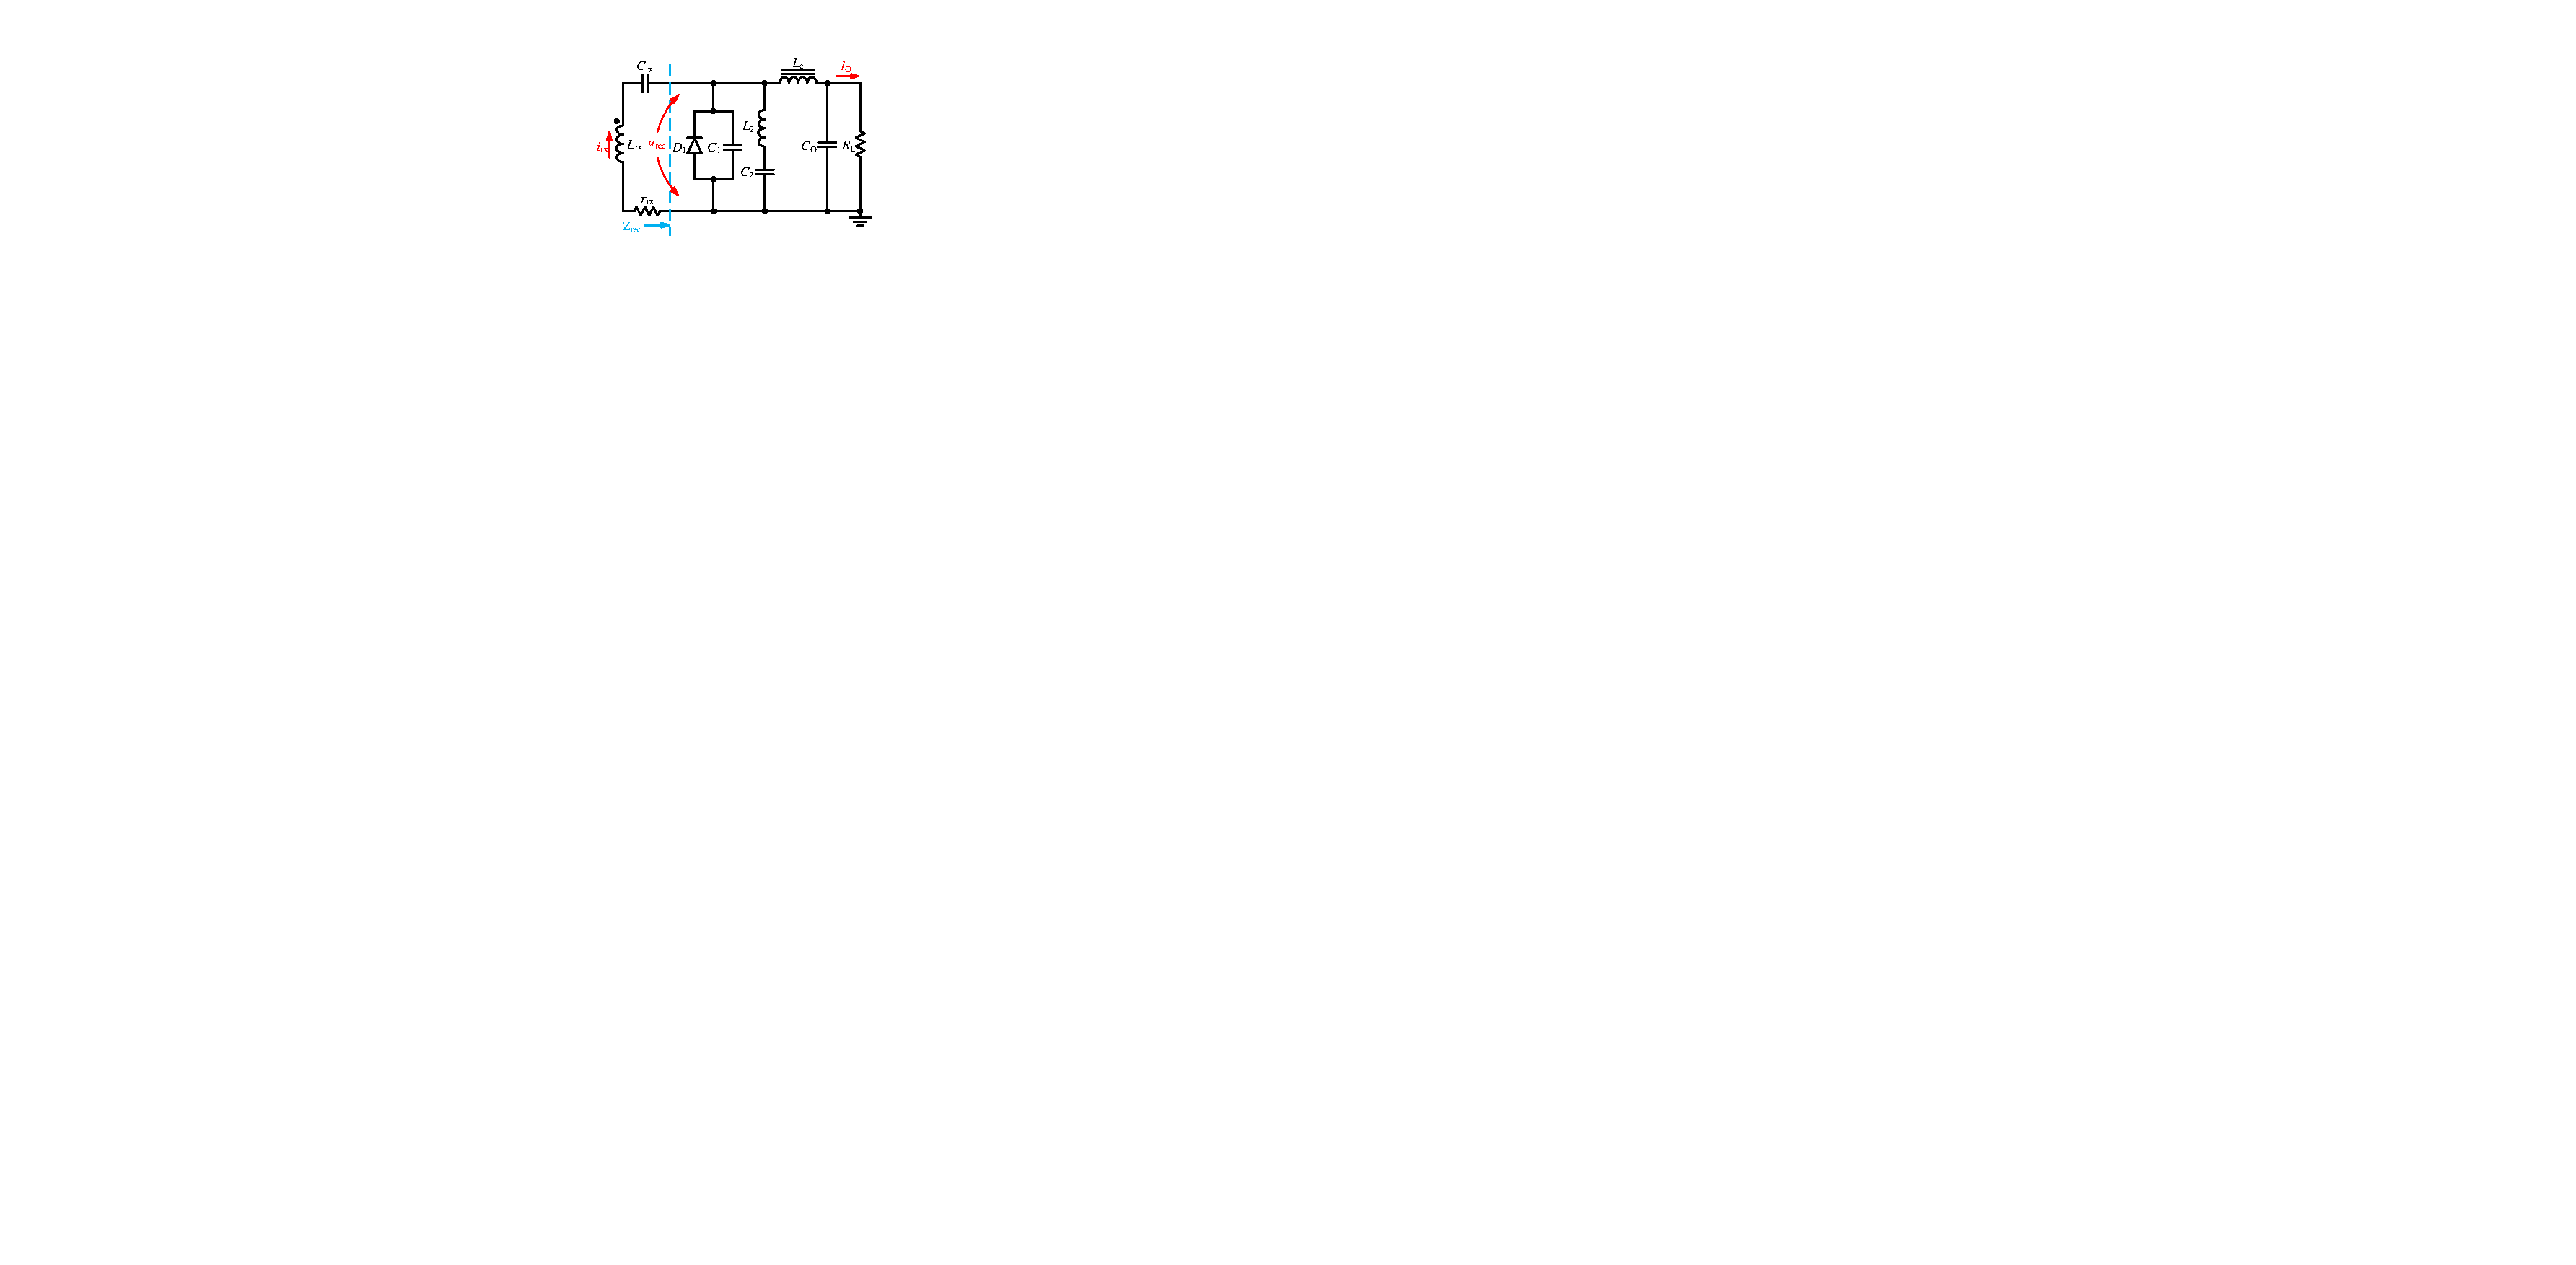
\includegraphics[width=2in]{FiguresEdge/RectifierEF.pdf}}
	\subfigure[]{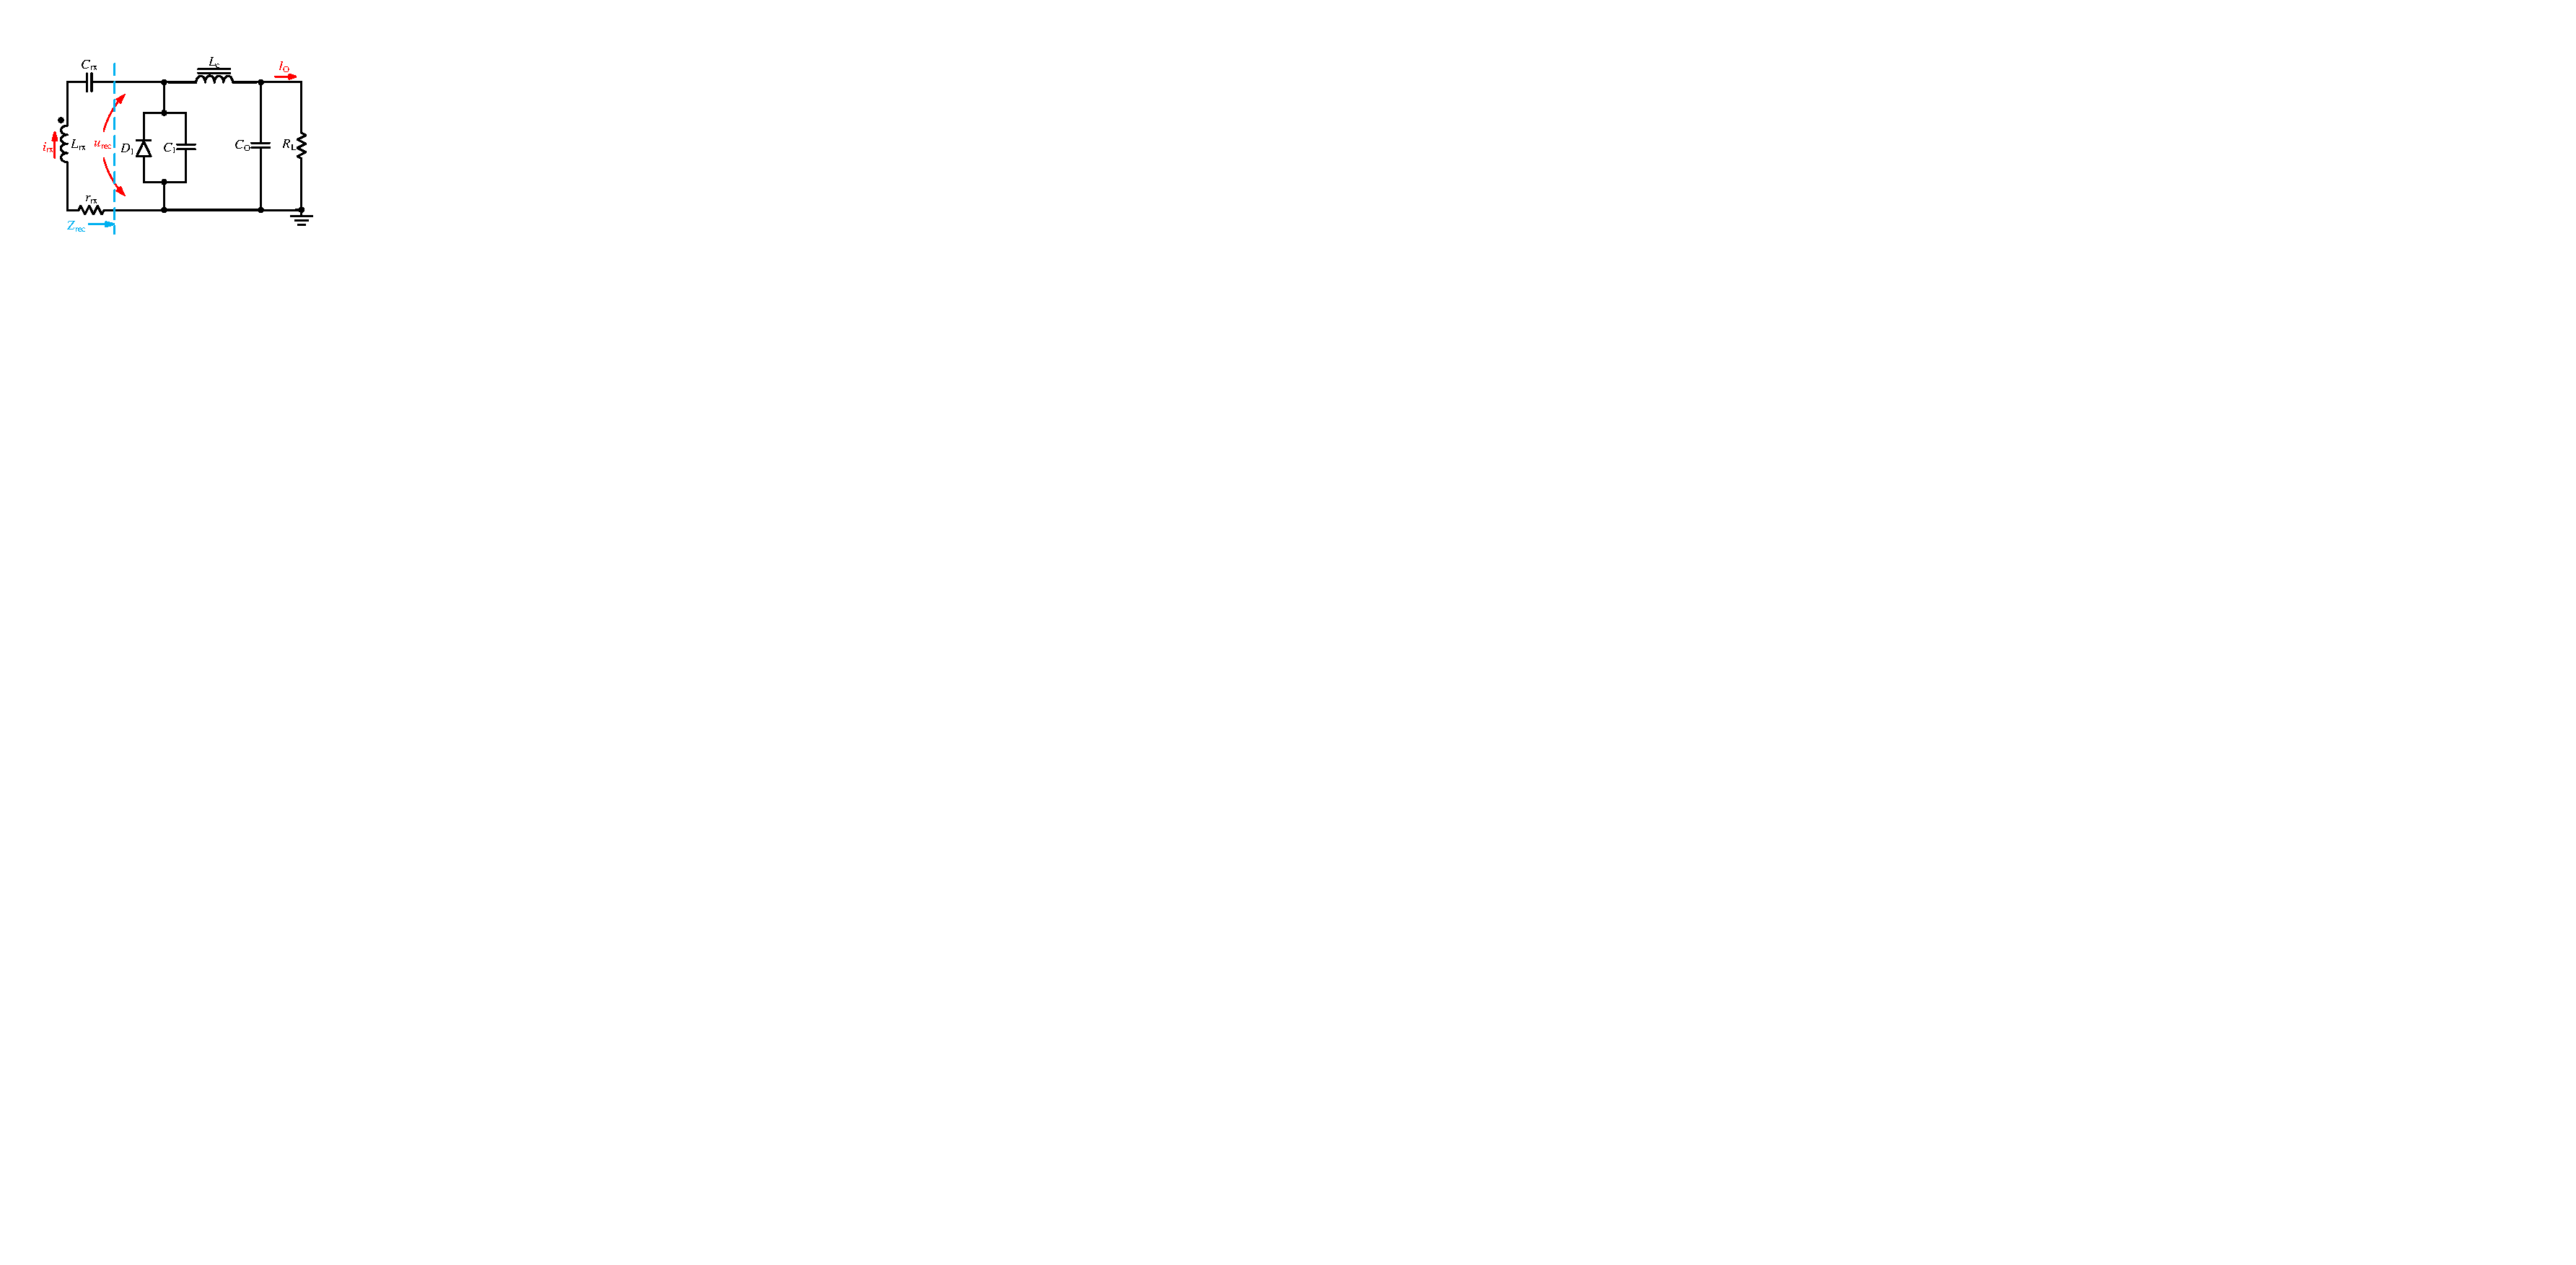
\includegraphics[width=2in]{FiguresEdge/RectifierHalfwave.pdf}}
	\caption{Class E family of rectifiers. (a) Full-wave rectifier. (b) Class EF rectifier. (c) Half-wave rectifier.}
	\label{fig:ClassEfamilyrectifier}
\end{figure}

\ifx\allfiles\undefined
	\onehalfspacing
	\bibliographystyle{chicago}
	%****************************************************************
	%=========This is the file that contains your bibliography entries=======
	%****************************************************************
	\bibliography{HuanBib}
	%=======================================================
	\end{document}
\fi

%\cleardoublepage
%\ifx\allfiles\undefined
	\include{Config} %deifne the using package and the paper layout
	\begin{document}
\else
	
\fi
\chapter{Chapter2 Name}
\section{Overview}
Here is the overview of chapter2. Here is the overview of chapter2. Here is the overview of chapter2. Here is the overview of chapter2

Here is the overview of chapter2. Here is the overview of chapter2. Here is the overview of chapter2. Here is the overview of chapter2

Here is the overview of chapter2. Here is the overview of chapter2. Here is the overview of chapter2. Here is the overview of chapter2

Here is the overview of chapter2. Here is the overview of chapter2. Here is the overview of chapter2. Here is the overview of chapter2

Here is the overview of chapter2. Here is the overview of chapter2. Here is the overview of chapter2. Here is the overview of chapter2

Here is the overview of chapter2. Here is the overview of chapter2. Here is the overview of chapter2. Here is the overview of chapter2

Here is the overview of chapter2. Here is the overview of chapter2. Here is the overview of chapter2. Here is the overview of chapter2

Here is the overview of chapter2. Here is the overview of chapter2. Here is the overview of chapter2. Here is the overview of chapter2
\begin{figure}[!htb]
	\centering
	\subfigure[]{\includegraphics[width=2in]{FiguresEdge/RectifierFullWave.pdf}}
	\subfigure[]{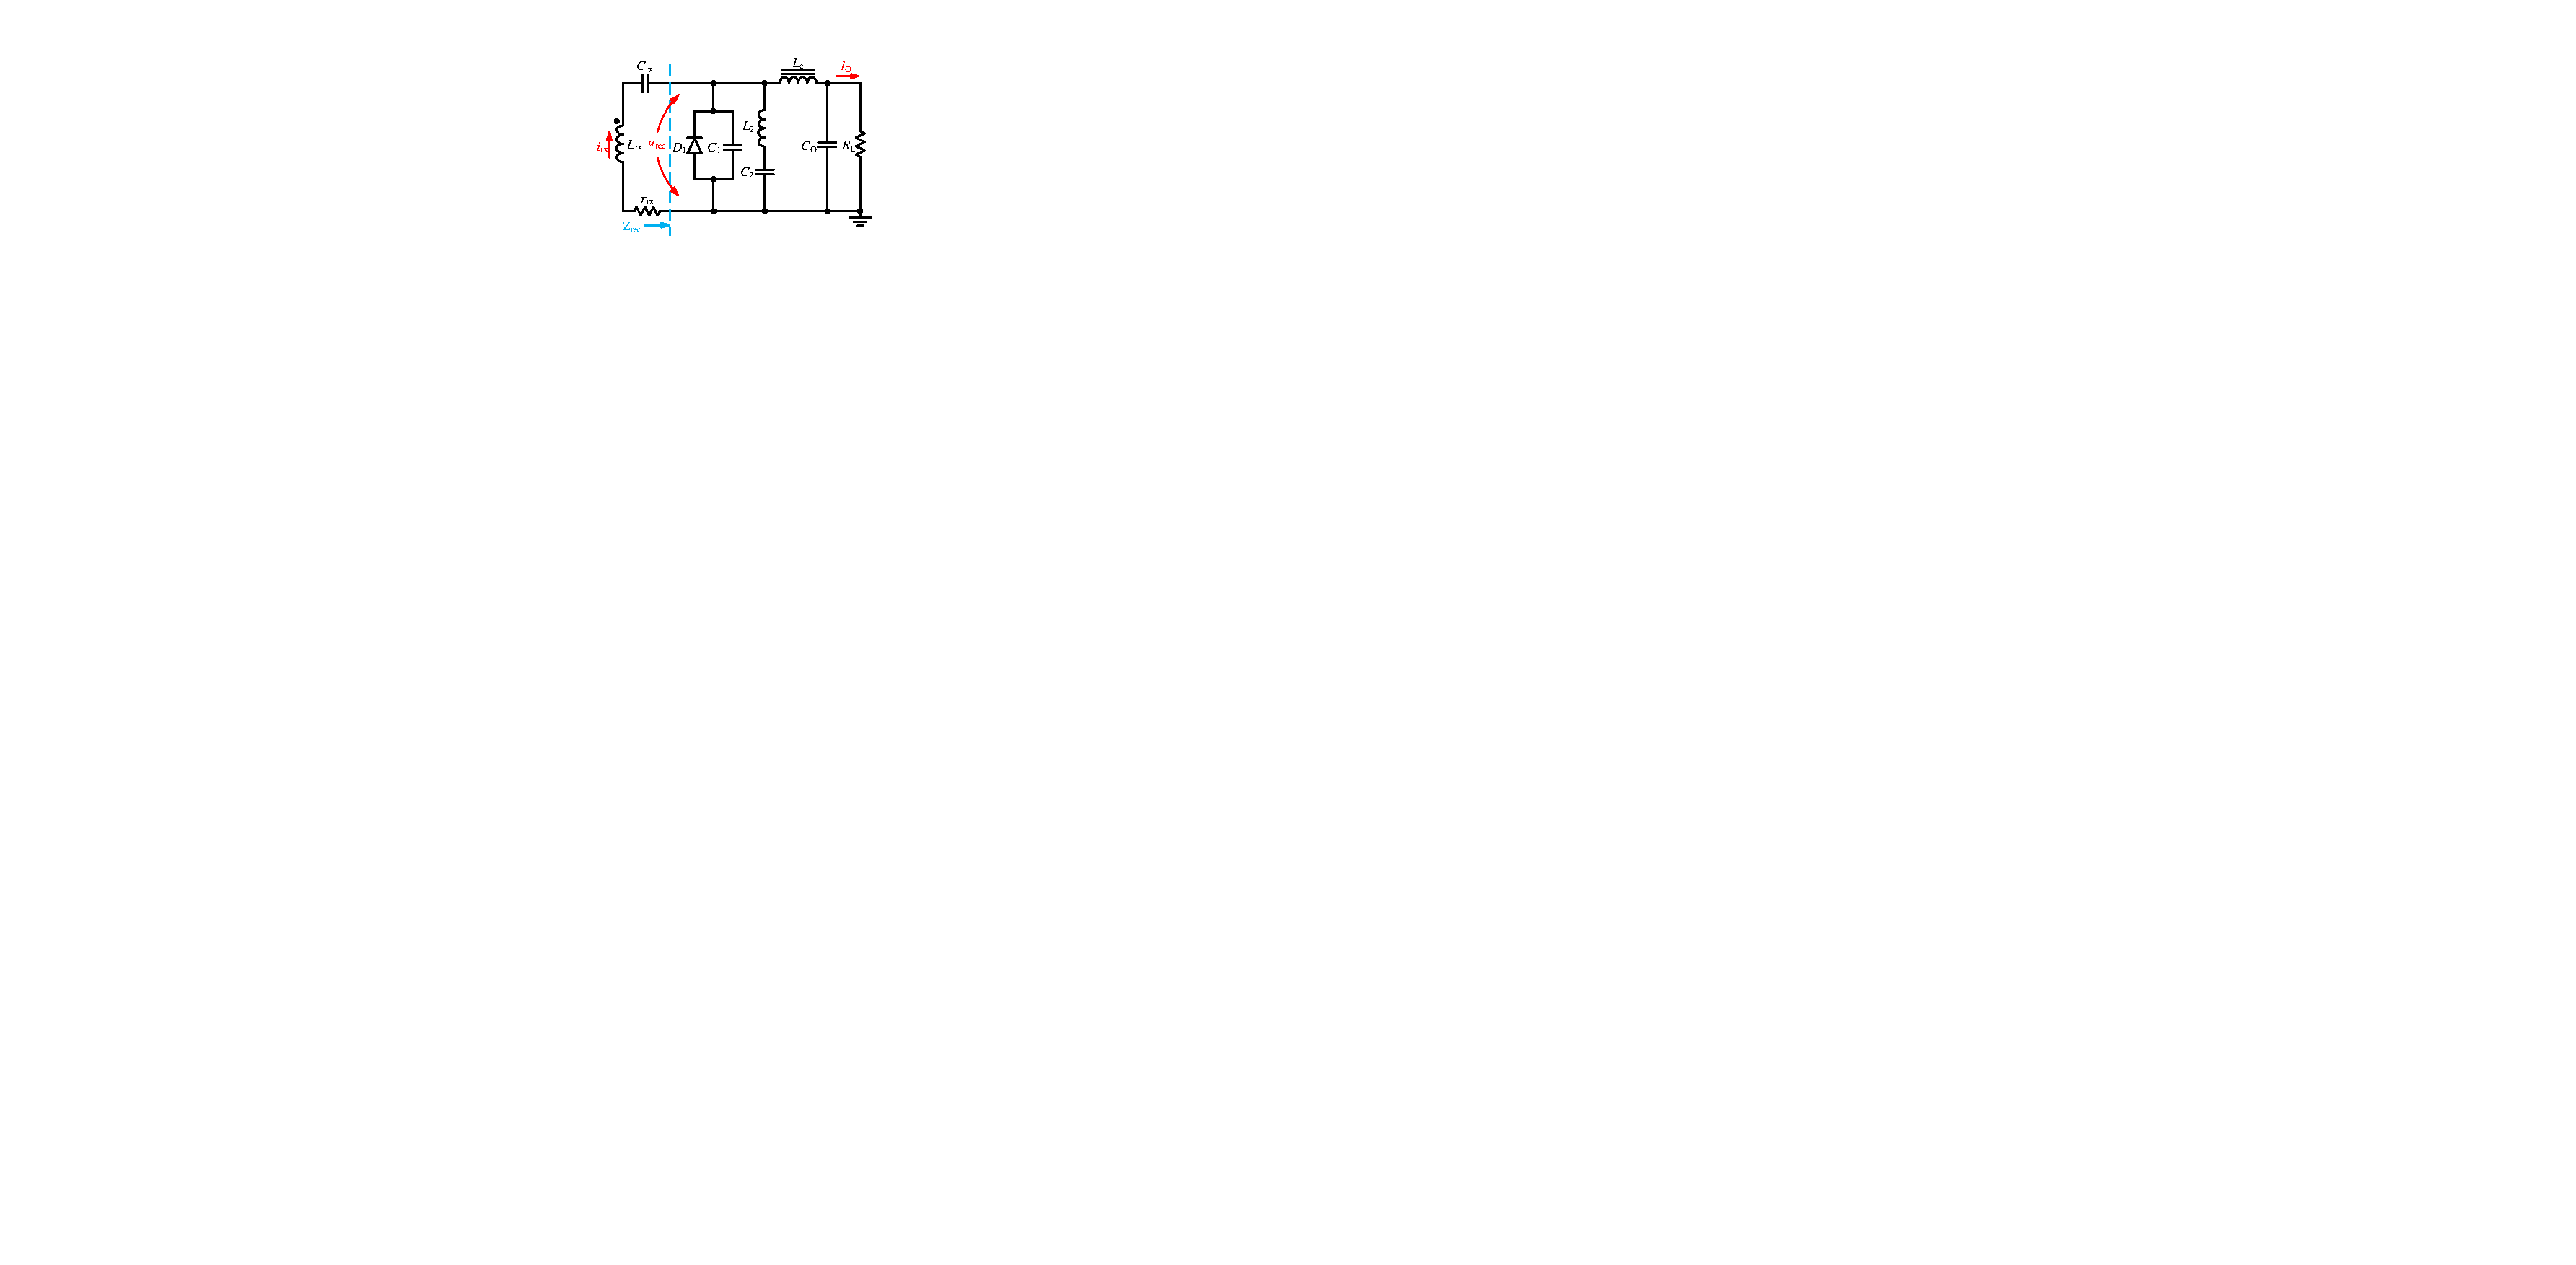
\includegraphics[width=2in]{FiguresEdge/RectifierEF.pdf}}
	\subfigure[]{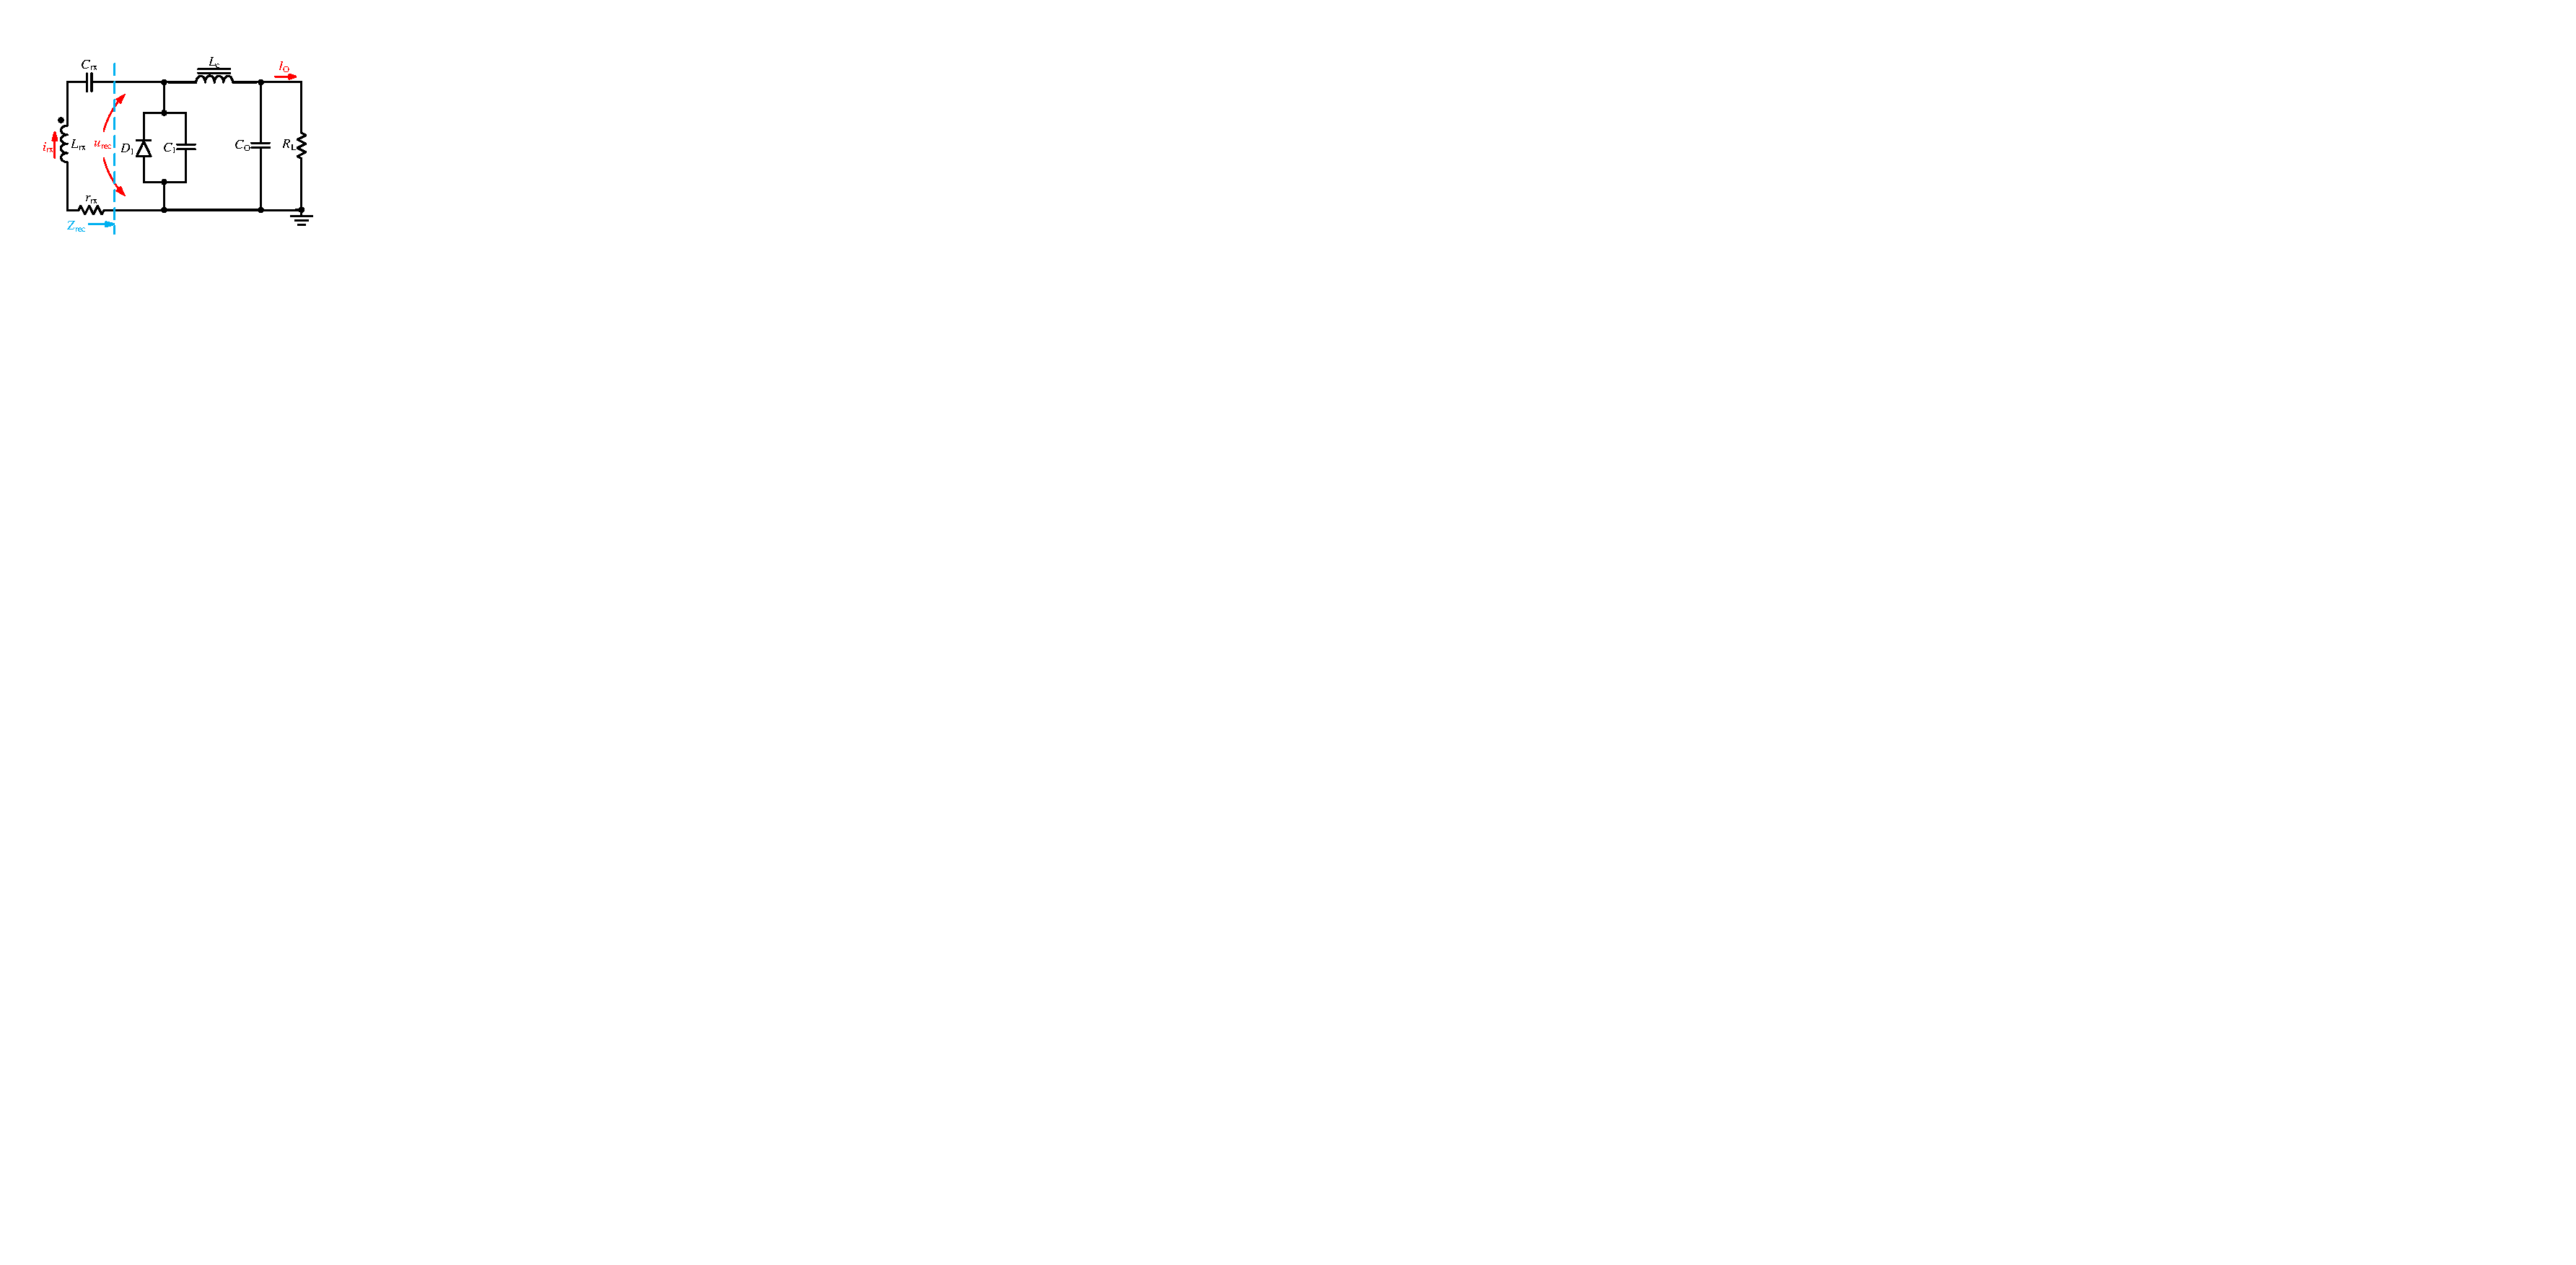
\includegraphics[width=2in]{FiguresEdge/RectifierHalfwave.pdf}}
	\caption{Class E family of rectifiers. (a) Full-wave rectifier. (b) Class EF rectifier. (c) Half-wave rectifier.}
	\label{fig:ClassEfamilyrectifier}
\end{figure}





\ifx\allfiles\undefined
	\onehalfspacing
	\bibliographystyle{chicago}
	%****************************************************************
	%=========This is the file that contains your bibliography entries=======
	%****************************************************************
	\bibliography{HuanBib}
	%=======================================================
	\end{document}
\fi=======================================

%\cleardoublepage
%%\ifx\allfiles\undefined
	\include{Config} %deifne the using package and the paper layout
	\begin{document}
\else
	
\fi
\chapter{Chapter3 Name}
\section{Overview}
Here is the overview of chapter3. Here is the overview of chapter3. Here is the overview of chapter3. Here is the overview of chapter3.

Here is the overview of chapter3. Here is the overview of chapter3. Here is the overview of chapter3. Here is the overview of chapter3.

Here is the overview of chapter3. Here is the overview of chapter3. Here is the overview of chapter3. Here is the overview of chapter3.

Here is the overview of chapter3. Here is the overview of chapter3. Here is the overview of chapter3. Here is the overview of chapter3.

Here is the overview of chapter3. Here is the overview of chapter3. Here is the overview of chapter3. Here is the overview of chapter3.

Here is the overview of chapter3. Here is the overview of chapter3. Here is the overview of chapter3. Here is the overview of chapter3.


\section{Section3}
\label{sec:ModularMRSystem}

\subsection{Modular Architecture}
ABCDE

\ifx\allfiles\undefined
	\onehalfspacing
	\bibliographystyle{chicago}
	%****************************************************************
	%=========This is the file that contains your bibliography entries=======
	%****************************************************************
	\bibliography{HuanBib}
	%=======================================================
	\end{document}
\fi
%%\cleardoublepage
%%\ifx\allfiles\undefined
	\include{Config}
	\begin{document}
\else
	
\fi
\chapter{Current Status and Working Plan}
\section{Overview}
Here is the overview. Here is the overview Here is the overview. Here is the overview. Here is the overview.

Here is the overview. Here is the overview Here is the overview. Here is the overview. Here is the overview

Here is the overview. Here is the overview Here is the overview. Here is the overview. Here is the overview

Here is the overview. Here is the overview Here is the overview. Here is the overview. Here is the overview

Here is the overview. Here is the overview Here is the overview. Here is the overview. Here is the overview

Here is the overview. Here is the overview Here is the overview. Here is the overview. Here is the overview
\section{Summary}\label{sec:Chapter4summary}
Here is the Summary.

\ifx\allfiles\undefined
	\onehalfspacing
	\bibliographystyle{chicago}
	%****************************************************************
	%=========This is the file that contains your bibliography entries=======
	%****************************************************************
	\bibliography{HuanBib}
	%=======================================================
	\end{document}
\fi



%%\cleardoublepage
%%\include{Chapter5}
%%\cleardoublepage
%\include{Conclusion}
%\cleardoublepage
%\chapter*{ACKNOWLEDGEMENT}

Here I would like to thank all the individuals who provide your kind supports and assistances to me and finally make this dissertation possible. It is hard to use words to express my gratitude to all of you.

Foremost, I want to express my heartfelt thanks to my Ph.D supervisor Prof.Chengbin Ma. His wisdom, knowledge, and encouragement really make me to mature as a qualified researcher.
Without his guidance, it is hard for me to make all the accomplishments what I have already achieved. 

Moreover, I would like to express my gratitude to my dissertation committee members, Prof. Houjun Tang, Prof. Jigang Wu, Prof. Mian Li, and Prof. Xinen Zhu. Their detailed guidance and insightful comments are very helpful to further improve the quality of this dissertation and make it more solid, both in terms of technical contents and readability. Also, many thanks to Prof. Patrick Chi-Kwong LUK and Dr. Songnan Yang for their worthful guidance and advice on my research works, especially at the very beginning of my research.

And then, I am grateful to all my lab mates for their selfless helps. I am very enjoy the time working with them all. I also thank the JI staffs for your kind supports throughout my Ph.D program.

Finally, I want to give the special thanks to my family, especially my wife and my son. I will never forget the debt I owe you for your gratuitous support and understanding in the past three years. For this sake, I dedicate the dissertation to you.





%\cleardoublepage
%\include{Appendix}
%\cleardoublepage
%\onehalfspacing
%\bibliographystyle{chicago}
%%****************************************************************
%%=========This is the file that contains your bibliography entries=======
%%****************************************************************
%\bibliography{References}
%%=======================================================
%\end{document}
 %deifne the using package and the paper layout
	\begin{document}
\else
	
\fi
\chapter{Chapter3 Name}
\section{Overview}
Here is the overview of chapter3. Here is the overview of chapter3. Here is the overview of chapter3. Here is the overview of chapter3.

Here is the overview of chapter3. Here is the overview of chapter3. Here is the overview of chapter3. Here is the overview of chapter3.

Here is the overview of chapter3. Here is the overview of chapter3. Here is the overview of chapter3. Here is the overview of chapter3.

Here is the overview of chapter3. Here is the overview of chapter3. Here is the overview of chapter3. Here is the overview of chapter3.

Here is the overview of chapter3. Here is the overview of chapter3. Here is the overview of chapter3. Here is the overview of chapter3.

Here is the overview of chapter3. Here is the overview of chapter3. Here is the overview of chapter3. Here is the overview of chapter3.


\section{Section3}
\label{sec:ModularMRSystem}

\subsection{Modular Architecture}
ABCDE

\ifx\allfiles\undefined
	\onehalfspacing
	\bibliographystyle{chicago}
	%****************************************************************
	%=========This is the file that contains your bibliography entries=======
	%****************************************************************
	\bibliography{HuanBib}
	%=======================================================
	\end{document}
\fi
%%\cleardoublepage
%%\ifx\allfiles\undefined
	\documentclass[12pt,a4paper,twoside,openright]{report}
%
%-----Packages
%
\usepackage[english]{babel}
\usepackage{setspace}
\usepackage[T1]{fontenc}
\usepackage[latin1]{inputenc}
\usepackage[intlimits]{amsmath}
\usepackage{amsfonts,amssymb}
\usepackage{natbib}
\usepackage[normalsize,bf]{caption}
\usepackage[dvips]{graphicx}
\usepackage{color}
\usepackage[breaklinks,linktocpage]{hyperref}
\usepackage{fancyhdr}
\usepackage{setspace}
\usepackage{subfigure}
\usepackage{float}
\usepackage{lettrine}
\usepackage{comment}
\usepackage{pifont}
\usepackage{soul, color}  %\hl
\usepackage{booktabs}	  %\toprule in table
\usepackage{tabularx}	  %\tabular
\usepackage{multicol}	  %table col
\usepackage{multirow}	  %table row
\usepackage{diagbox}

\newcommand{\hlg}[2][green]{{\sethlcolor{#1}\hl{#2}}}
\newcommand{\tabincell}[2]{\begin{tabular}{@{}#1@{}}#2\end{tabular}}
\sloppy\par
%****************************************************************
% ===========Optional packages (uncomment as needed)=============
%****************************************************************
\usepackage{wrapfig}
%\usepackage{makeidx}
\usepackage{amsbsy}
\usepackage{latexsym}
\usepackage{amsthm}
\usepackage{datatool}
%\usepackage{glossary}
\usepackage{glossaries}
%\makeglossary
%\makeglossaries


%=======================================================
%
%-----Layout
%
\onehalfspacing
\hoffset = -1 in
\voffset= -1 in
%
%-----Set margins for a4 paper
%
\topmargin = 3.0cm
\textwidth = 17cm
\textheight = 22cm
\oddsidemargin =  2cm
\evensidemargin = 2cm
%
%-----Headers and Footers
%
\pagestyle{fancyplain}
\renewcommand{\chaptermark}[1]%
{\markboth{#1}{}}
\renewcommand{\sectionmark}[1]%
{\markright{\thesection\ -- #1}}
\lhead[\fancyplain{}{\thepage}]%
{\fancyplain{}{\rightmark}}
\rhead[\fancyplain{}{\leftmark}]%
{\fancyplain{}{\thepage}}
\cfoot{}
%
%-----No headers on empty pages before new chapter
%
\makeatletter
\def\cleardoublepage{\clearpage\if@twoside \ifodd\c@page\else
	\hbox{}
	\thispagestyle{plain}
	\newpage
	\if@twocolumn\hbox{}\newpage\fi\fi\fi}
\makeatother \clearpage{\pagestyle{plain}\cleardoublepage}
%
%-----Footnotes
%
\renewcommand{\thefootnote}{\fnsymbol{footnote}} % Footnotes are marked with symbols instead of literals
\setlength{\textfloatsep}{8pt plus 4pt minus 4pt}        % Separation of floats from text
\renewcommand{\bibnumfmt}[1]{{\scriptsize #1}}
\setlength{\bibhang}{2em}
%
%-----Define Horizontal rule
%
\newcommand{\HRule}{\rule{\textwidth}{0.5mm}}
%
%-----Define Hyperlink colors
%
\definecolor{darkred}{rgb}{0.25,0,0}
\definecolor{darkgreen}{rgb}{0,0.25,0}
\definecolor{darkblue}{rgb}{0,0,0.5}
\hypersetup{colorlinks,linkcolor=black,filecolor=black,urlcolor=darkblue,citecolor=black}
\usepackage{breakurl}
%****************************************************************
% ===========Add user definitions as needed=====================
%****************************************************************
%\include{definitions}
\newtheorem{theorem}{Theorem}[chapter]
\newtheorem{principle}{Principle}[chapter]
\newtheorem{algorithm}{Algorithm}[chapter]
\newtheorem{law}{Law}
%\theoremstyle{plain}  % Default
\theoremstyle{definition}
%\theoremstyle{remark}
\newtheorem{problem}{Problem}[chapter]
\newtheorem{example}{Example}[chapter]
\newtheorem{definition}{Definition}[chapter]




%%***********Config file orginal backup*********
%\immediate\write18{makeindex \jobname.nlo -s nomencl.ist -o \jobname.nls}
%\documentclass[12pt,a4paper,twoside,openright]{report}
%%
%%-----Packages
%%
%\usepackage[english]{babel}
%\usepackage{setspace}
%\usepackage[T1]{fontenc}
%\usepackage[latin1]{inputenc}
%\usepackage[intlimits]{amsmath}
%\usepackage{amsfonts,amssymb}
%\usepackage{natbib}
%\usepackage[normalsize,bf]{caption}
%\usepackage[dvips]{graphicx}
%%\usepackage{color}
%%\usepackage{mathdots}
%%\usepackage{mathtools}
%%\usepackage{booktabs}
%%\usepackage{multirow}
%%\usepackage{ps2pdf}
%\usepackage{epstopdf}
%\usepackage[breaklinks,linktocpage]{hyperref}
%\usepackage{fancyhdr}
%\usepackage{setspace}
%\usepackage{subfigure}
%\usepackage{lettrine}
%\newcommand{\tabincell}[2]{\begin{tabular}{@{}#1@{}}#2\end{tabular}}
%\sloppy\par
%%****************************************************************
%% ===========Optional packages (uncomment as needed)=============
%%****************************************************************
%\usepackage{wrapfig}
%%\usepackage{makeidx}
%\usepackage{amsbsy}
%\usepackage{latexsym}
%\usepackage{amsthm}
%\usepackage{datatool}
%\usepackage{nomencl}
%\makenomenclature
%\usepackage{glossaries}
%\makeglossaries
%\usepackage{ifthen}
%\usepackage{graphicx}
%\usepackage{color, soul}
%%\usepackage{wasysym}
%%\usepackage{psfrag}
%%\usepackage{subfig}
%%\usepackage{pifont}
%%\usepackage{longtable}
%%\setlength\LTleft{0pt}
%%\setlength\LTright{0pt}
%%=======================================================
%%
%%-----Layout
%%
%\onehalfspacing
%\hoffset = -1 in
%\voffset= -1 in
%%
%%-----Set margins for a4 paper
%%
%\topmargin = 3.0cm
%\textwidth = 17cm
%\textheight = 22cm
%\oddsidemargin =  2cm
%\evensidemargin = 2cm
%%
%%-----Headers and Footers
%%
%\pagestyle{fancyplain}
%\renewcommand{\chaptermark}[1]%
%            {\markboth{#1}{}}
%\renewcommand{\sectionmark}[1]%
%            {\markright{\thesection\ -- #1}}
%\lhead[\fancyplain{}{\thepage}]%
%      {\fancyplain{}{\rightmark}}
%\rhead[\fancyplain{}{\leftmark}]%
%     {\fancyplain{}{\thepage}}
%\cfoot{}
%%
%%-----No headers on empty pages before new chapter
%%
%\makeatletter
%\def\cleardoublepage{\clearpage\if@twoside \ifodd\c@page\else
%    \hbox{}
%    \thispagestyle{plain}
%    \newpage
%    \if@twocolumn\hbox{}\newpage\fi\fi\fi}
%\makeatother \clearpage{\pagestyle{plain}\cleardoublepage}
%%
%%-----Footnotes
%%
%\renewcommand{\thefootnote}{\fnsymbol{footnote}} % Footnotes are marked with symbols instead of literals
%\setlength{\textfloatsep}{8pt plus 4pt minus 4pt}        % Separation of floats from text
%\renewcommand{\bibnumfmt}[1]{{\scriptsize #1}}
%\setlength{\bibhang}{2em}
%%
%%-----Define Horizontal rule
%%
%\newcommand{\HRule}{\rule{\textwidth}{0.5mm}}
%%
%%-----Define Hyperlink colors
%%
%\definecolor{darkred}{rgb}{0.25,0,0}
%\definecolor{darkgreen}{rgb}{0,0.25,0}
%\definecolor{darkblue}{rgb}{0,0,0.5}
%\hypersetup{colorlinks,linkcolor=black,filecolor=black,urlcolor=darkblue,citecolor=black}
%\usepackage{breakurl}
%
%%****************************************************************
%% ===========Add user definitions as needed=====================
%%****************************************************************
%\include{definitions}
%\newtheorem{theorem}{Theorem}[chapter]
%\newtheorem{principle}{Principle}[chapter]
%%\newtheorem{algorithm}{Algorithm}[chapter]
%\newtheorem{law}{Law}
%%\theoremstyle{plain}  % Default
%\theoremstyle{definition}
%%\theoremstyle{remark}
%\newtheorem{problem}{Problem}[chapter]
%\newtheorem{example}{Example}[chapter]
%\newtheorem{definition}{Definition}[chapter]
%%=======================================================
%%%%%%%%%%%%%
%%-----Begin Document
%%%%%%%%%%%%%
%\begin{document}
%\pagenumbering{roman}
%%
%%-----Title page
%%
%
%\begin{titlepage}
%\noindent {\bf Shanghai Jiao Tong University \\
%University of Michigan- Shanghai Jiao Tong University Joint Institute}\\
%\noindent \HRule \vspace{0.0455\textheight}
%%****************************************************************
%% ===========Edit the following lines to get the right title============
%%****************************************************************
%\begin{center}
%{\huge \bf Proposal Name}\\[0.016\textheight]
%{\Large \bf Doctoral Dissertation Proposal} \\[0.032\textheight]
%\large{by} \\[0.032\textheight] \Large{ \bf Jibin Song}\\
%%=======================================================
%\vspace{5cm}
%\normalsize{A proposal submitted in satisfaction of the \\
%requirements for the degree of Doctor of Philosophy in \\
%Control Science and Engineering at Shanghai Jiao Tong University}
%\HRule \\[0.023\textheight]
%%****************************************************************
%%======Edit the following lines to get the right committee members======
%%****************************************************************
%\begin{tabular*}{\textwidth}{@{}l@{\extracolsep{\fill}}r@{}}
%\textbf{Committee in charge:} &  \textbf{Shanghai}\\
%\textbf{Professor XXX} &  \textbf{July, 2020}\\
%\textbf{Professor XXX} & \\
%\textbf{Professor XXX} & \\
%\textbf{Professor XXX} & \\
%\textbf{Professor XXX} & \\
%\end{tabular*}
%%=======================================================
%\end{center}
%\end{titlepage}
%
%%
%%-----Abstract
%%
%\thispagestyle{empty}
%\cleardoublepage
%%****************************************************************
%%===========Your abstract goes in the file Abstract.tex==============
%%****************************************************************
%
%
%
%\begin{abstract}
\noindent

Here is the abstract. Here is the abstract. Here is the abstract. Here is the abstract.

Here is the abstract. Here is the abstract. Here is the abstract. Here is the abstract.

Here is the abstract. Here is the abstract. Here is the abstract. Here is the abstract.

Here is the abstract. Here is the abstract. Here is the abstract. Here is the abstract.

Here is the abstract. Here is the abstract. Here is the abstract. Here is the abstract.

Here is the abstract. Here is the abstract. Here is the abstract. Here is the abstract.

Here is the abstract. Here is the abstract. Here is the abstract. Here is the abstract.

Here is the abstract. Here is the abstract. Here is the abstract. Here is the abstract.
\end{abstract}



%\cleardoublepage
%\newlength{\nomitemorigsep}
\setlength{\nomitemorigsep}{\nomitemsep}
\setlength{\nomitemsep}{-\parsep}
\makenomenclature
\renewcommand{\nomgroup}[1]{%
  \itemsep\nomitemorigsep%
  \ifthenelse{%
    \equal{#1}{A}%
  }{%
  \item[\textbf{Abbreviations}]%

  }{%
    \ifthenelse{\equal{#1}{S}}{%
    \item[\textbf{List of Symbols}]%

    }{}%
  }%
  \itemsep\nomitemsep
}
\renewcommand{\nomname}{Nomenclature}
\markboth{\MakeUppercase\nomname}{\MakeUppercase\nomname}
\printnomenclature[0.8in]
\nomenclature[A]{ADS}{Advanced Design System}
\nomenclature[A]{ESR}{Equivalent series resistance}
\nomenclature[A]{MOSFET}{Metal-oxide-semiconductor field effect transistor}
\nomenclature[A]{MWPT}{Multiple-receiver wrieless power transfer}
\nomenclature[A]{PA}{Power amplifier}
\nomenclature[A]{RF}{Radio frequency}
\nomenclature[A]{SRR}{Synchronous Resonant Rectifier}
\nomenclature[A]{WPT}{Wireless power transfer}
\nomenclature[A]{ZVS}{Zero-voltage-switching}




\nomenclature[S]{$C_{0}$}{Capacitor in resonant tank of Class E PA}
\nomenclature[S]{$C_{r}$}{Diode/switch shunt capacitor of Class E rectifier}
\nomenclature[S]{$C_{S}$}{Switch shunt capacitor of Class E PA}
\nomenclature[S]{$C_{rx}$}{Compensation capacitor of receiving coil}
\nomenclature[S]{$C_{tx}$}{Compensation capacitor of transmitting coil}
\nomenclature[S]{$k$}{Mutual inductance coefficient of coupling coils}
\nomenclature[S]{$k_{ij}$}{Mutual inductance coefficient between $i$-th and $j$-th coils in MWPT}
\nomenclature[S]{$L_{0}$}{Inductor in resonant tank of Class E PA}
\nomenclature[S]{$L_{rx}$}{Inductance of receiving coil}
\nomenclature[S]{$L_{tx}$}{Inductance of transmitting coil}
\nomenclature[S]{$M$}{Mutual inductance of coupling coils}
\nomenclature[S]{$M_{ij}$}{Mutual inductance between $i$-th and $j$-th coils in MWPT}
\nomenclature[S]{$r_{rx}$}{ESR of receiving coil}
\nomenclature[S]{$r_{tx}$}{ESR of transmitting coil}
\nomenclature[S]{$R_{L}$}{Dc load of rectifier}
\nomenclature[S]{$R_{rec}$}{Input resisance of rectifier}
\nomenclature[S]{$v_{DS}$}{Drain-source voltage of MOSFET}
\nomenclature[S]{$v_{GS}$}{Gate-source voltage of MOSFET}
\nomenclature[S]{$X_{rec}$}{Input reactance of rectifier}
\nomenclature[S]{$Z_{rec}$}{Input impedance of rectifier}
\nomenclature[S]{$Z_{coil}$}{Input impedance of transmitting coil}
\nomenclature[S]{$\eta_{PA}$}{Efficiency of PA}
\nomenclature[S]{$\eta_{rec}$}{Efficiency of rectifier}
\nomenclature[S]{$\eta_{sys}$}{Dc-dc efficiency of WPT system}
\nomenclature[S]{$\eta_{coil2load}$}{Power transfer efficiency from transmitting coil to dc load}


\cleardoublepage 







%\cleardoublepage
%%\printglossary
%%=======================================================
%%
%%-----Table of contents
%%
%%\clearpage
%\setcounter{tocdepth}{1}
%\setcounter{page}{1}
%\tableofcontents
%\doublespacing
%\listoffigures
%\doublespacing
%\listoftables
%\doublespacing
%
%
%
%
%
%\setcounter{page}{1}
%\pagenumbering{arabic}
%%****************************************************************
%%================Include each chapter in a different file===========
%%======For large theses, chapters should be in different directories=======
%%=============Add \cleardoublepage between each chapter==========
%%****************************************************************
%\ifx\allfiles\undefined   
	\include{Config} %deifne the using package and the paper layout
	\begin{document}
\else

\fi

\chapter{Introduction}
\section{Overview}
Here is the background~\citep{MHzcompact}
Here is the overview of chapter1. Here is the overview of chapter1. Here is the overview of chapter1. Here is the overview of CSD. 

Here is the overview of chapter1. Here is the overview of chapter1. Here is the overview of chapter1. Here is the overview of chapter1

Here is the overview of chapter1. Here is the overview of chapter1. Here is the overview of chapter1. Here is the overview of chapter1

Here is the overview of chapter1. Here is the overview of chapter1. Here is the overview of chapter1. Here is the overview of chapter1

Here is the overview of chapter1. Here is the overview of chapter1. Here is the overview of chapter1. Here is the overview of chapter1

Here is the overview of chapter1. Here is the overview of chapter1. Here is the overview of chapter1. Here is the overview of chapter1

Here is the overview of chapter1. Here is the overview of chapter1. Here is the overview of chapter1. Here is the overview of BAC

Here is the overview of chapter1. Here is the overview of chapter1. Here is the overview of chapter1. Here is the overview of chapter1

\begin{figure}[!htb]
	\centering
	\subfigure[]{\includegraphics[width=2in]{FiguresEdge/RectifierFullWave.pdf}}
	\subfigure[]{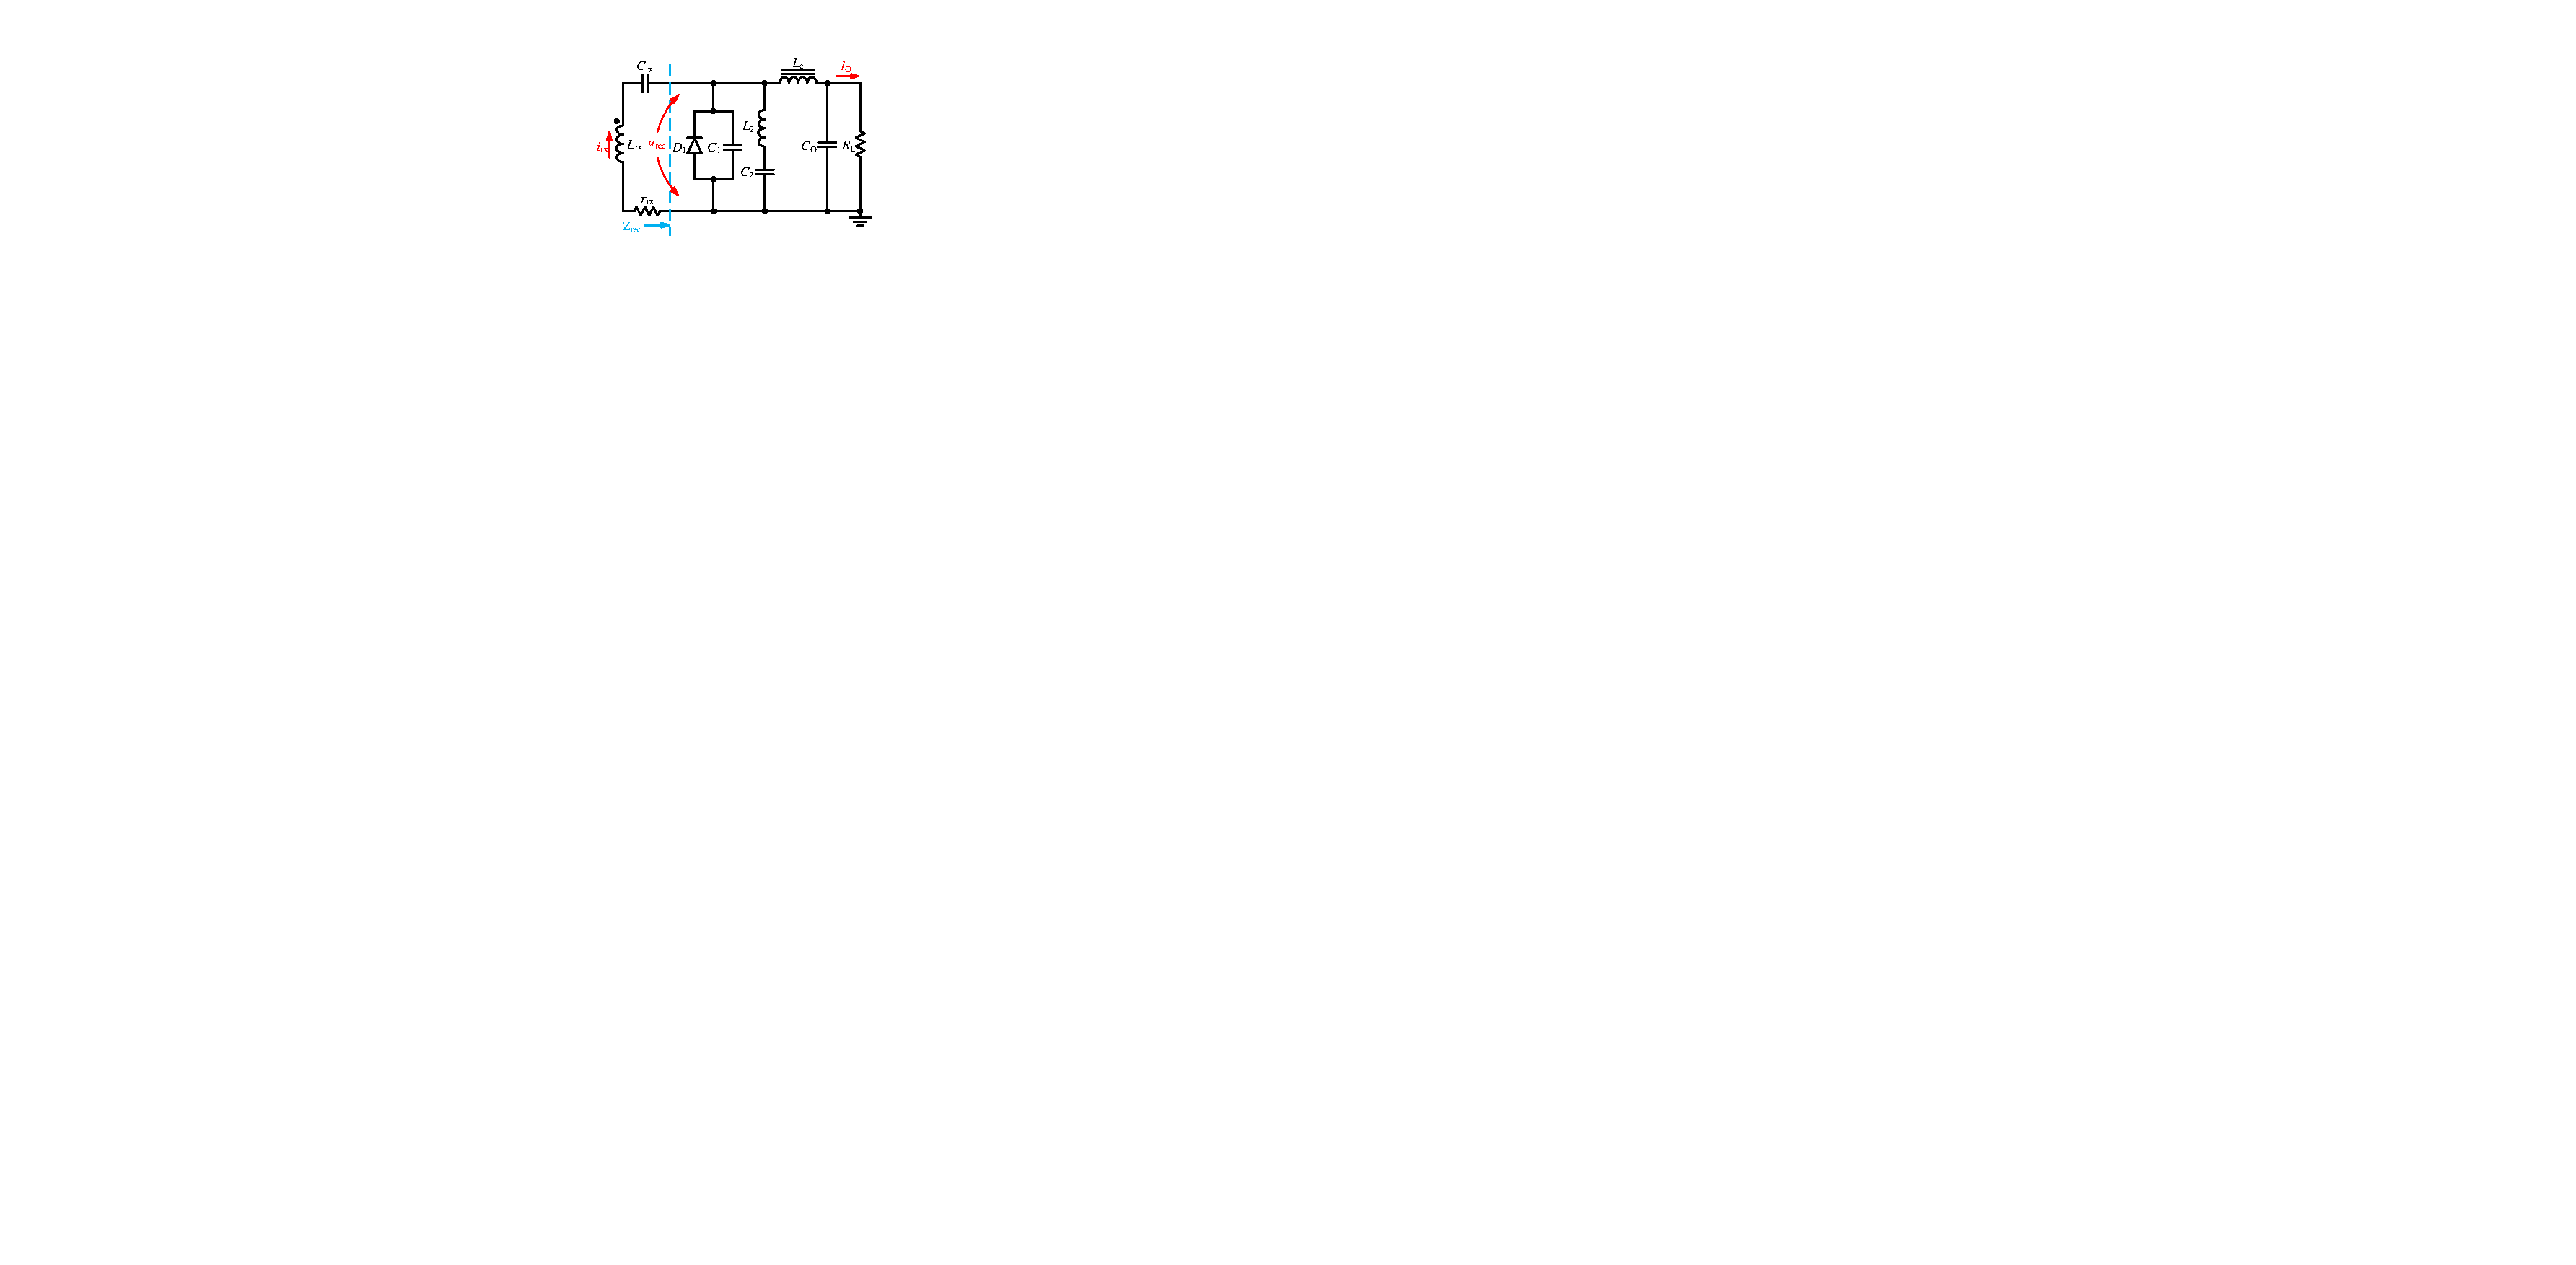
\includegraphics[width=2in]{FiguresEdge/RectifierEF.pdf}}
	\subfigure[]{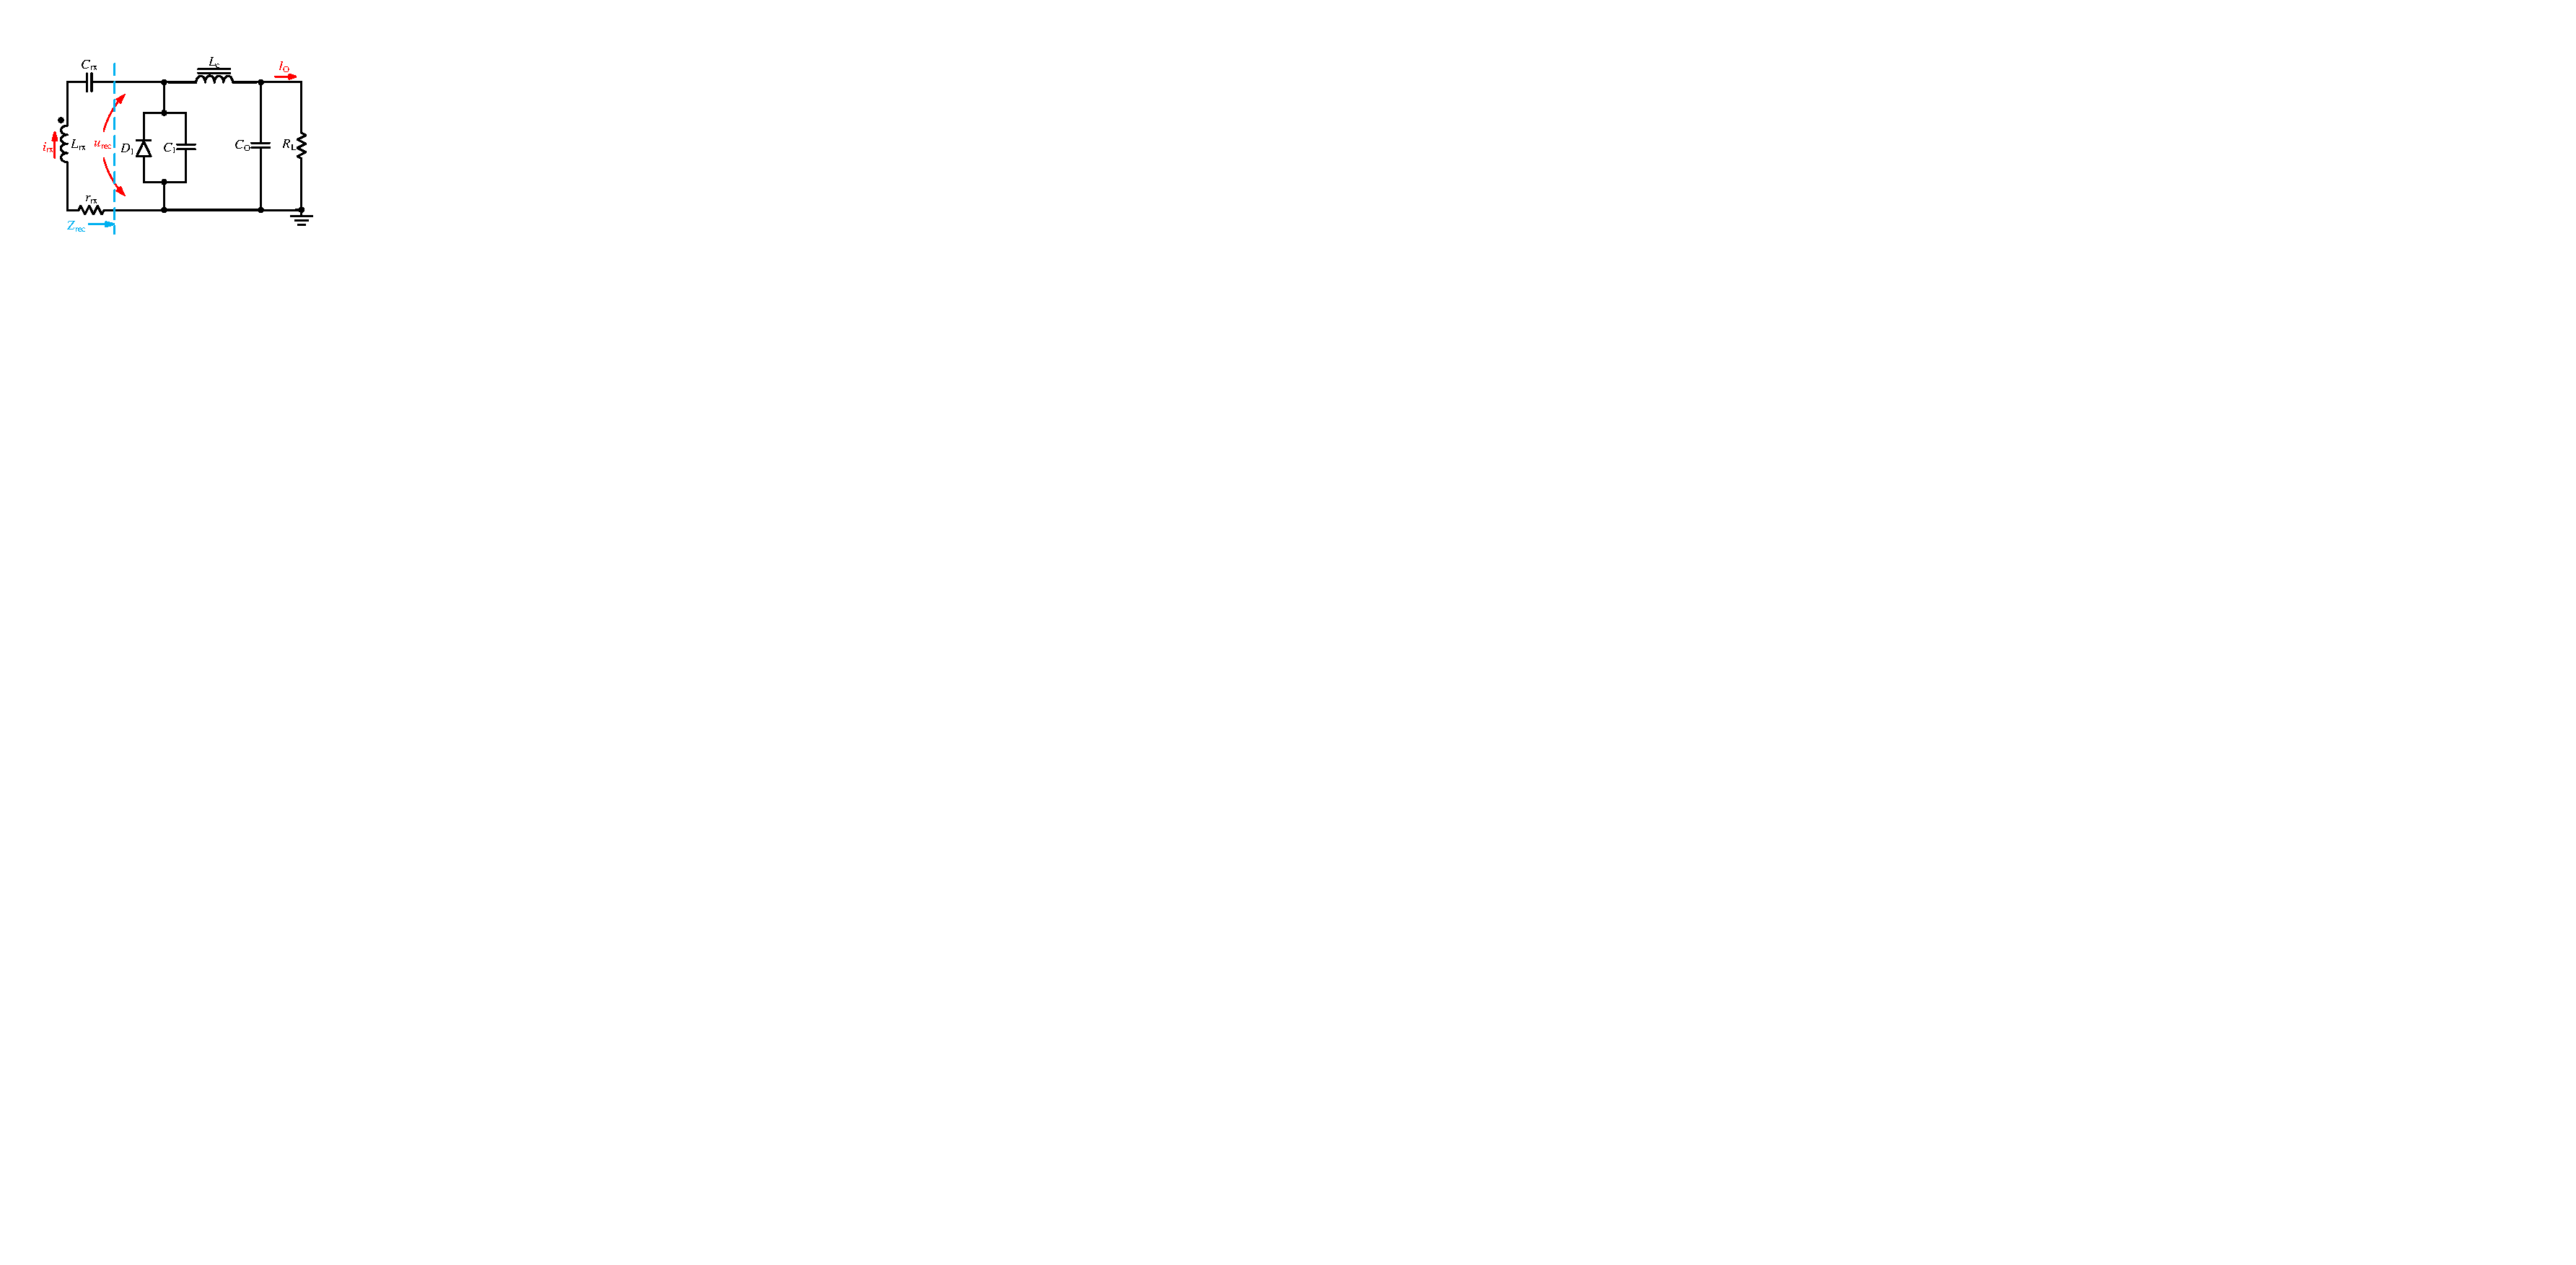
\includegraphics[width=2in]{FiguresEdge/RectifierHalfwave.pdf}}
	\caption{Class E family of rectifiers. (a) Full-wave rectifier. (b) Class EF rectifier. (c) Half-wave rectifier.}
	\label{fig:ClassEfamilyrectifier}
\end{figure}

\ifx\allfiles\undefined
	\onehalfspacing
	\bibliographystyle{chicago}
	%****************************************************************
	%=========This is the file that contains your bibliography entries=======
	%****************************************************************
	\bibliography{HuanBib}
	%=======================================================
	\end{document}
\fi

%\cleardoublepage
%\ifx\allfiles\undefined
	\include{Config} %deifne the using package and the paper layout
	\begin{document}
\else
	
\fi
\chapter{Chapter2 Name}
\section{Overview}
Here is the overview of chapter2. Here is the overview of chapter2. Here is the overview of chapter2. Here is the overview of chapter2

Here is the overview of chapter2. Here is the overview of chapter2. Here is the overview of chapter2. Here is the overview of chapter2

Here is the overview of chapter2. Here is the overview of chapter2. Here is the overview of chapter2. Here is the overview of chapter2

Here is the overview of chapter2. Here is the overview of chapter2. Here is the overview of chapter2. Here is the overview of chapter2

Here is the overview of chapter2. Here is the overview of chapter2. Here is the overview of chapter2. Here is the overview of chapter2

Here is the overview of chapter2. Here is the overview of chapter2. Here is the overview of chapter2. Here is the overview of chapter2

Here is the overview of chapter2. Here is the overview of chapter2. Here is the overview of chapter2. Here is the overview of chapter2

Here is the overview of chapter2. Here is the overview of chapter2. Here is the overview of chapter2. Here is the overview of chapter2
\begin{figure}[!htb]
	\centering
	\subfigure[]{\includegraphics[width=2in]{FiguresEdge/RectifierFullWave.pdf}}
	\subfigure[]{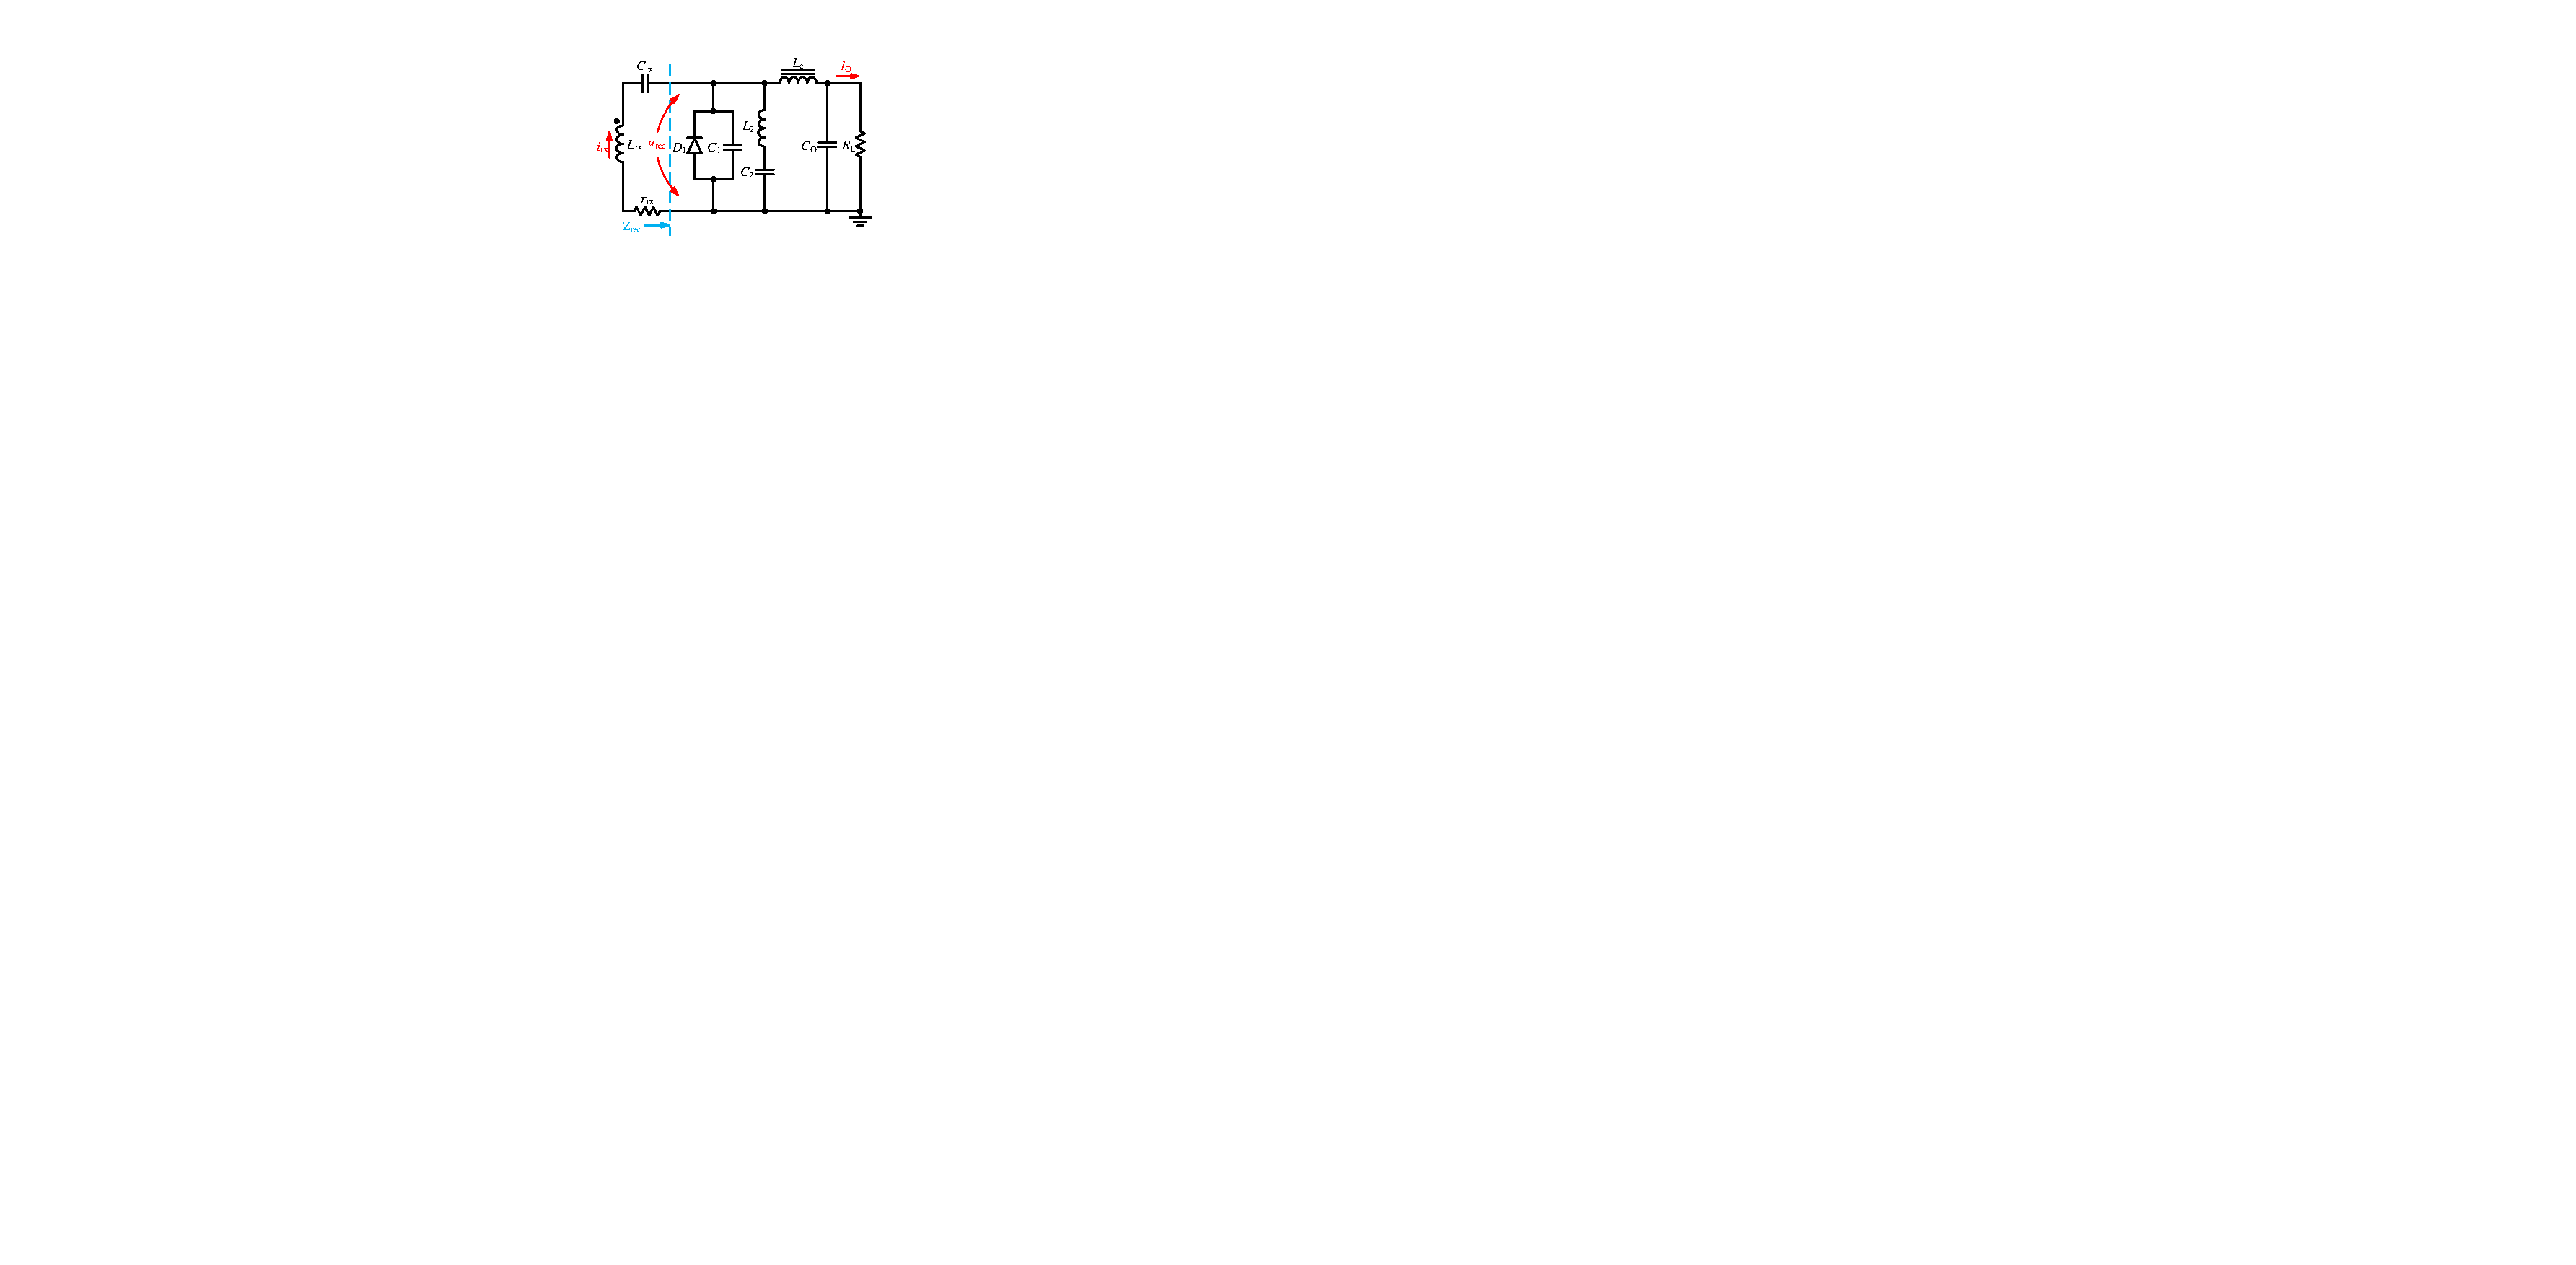
\includegraphics[width=2in]{FiguresEdge/RectifierEF.pdf}}
	\subfigure[]{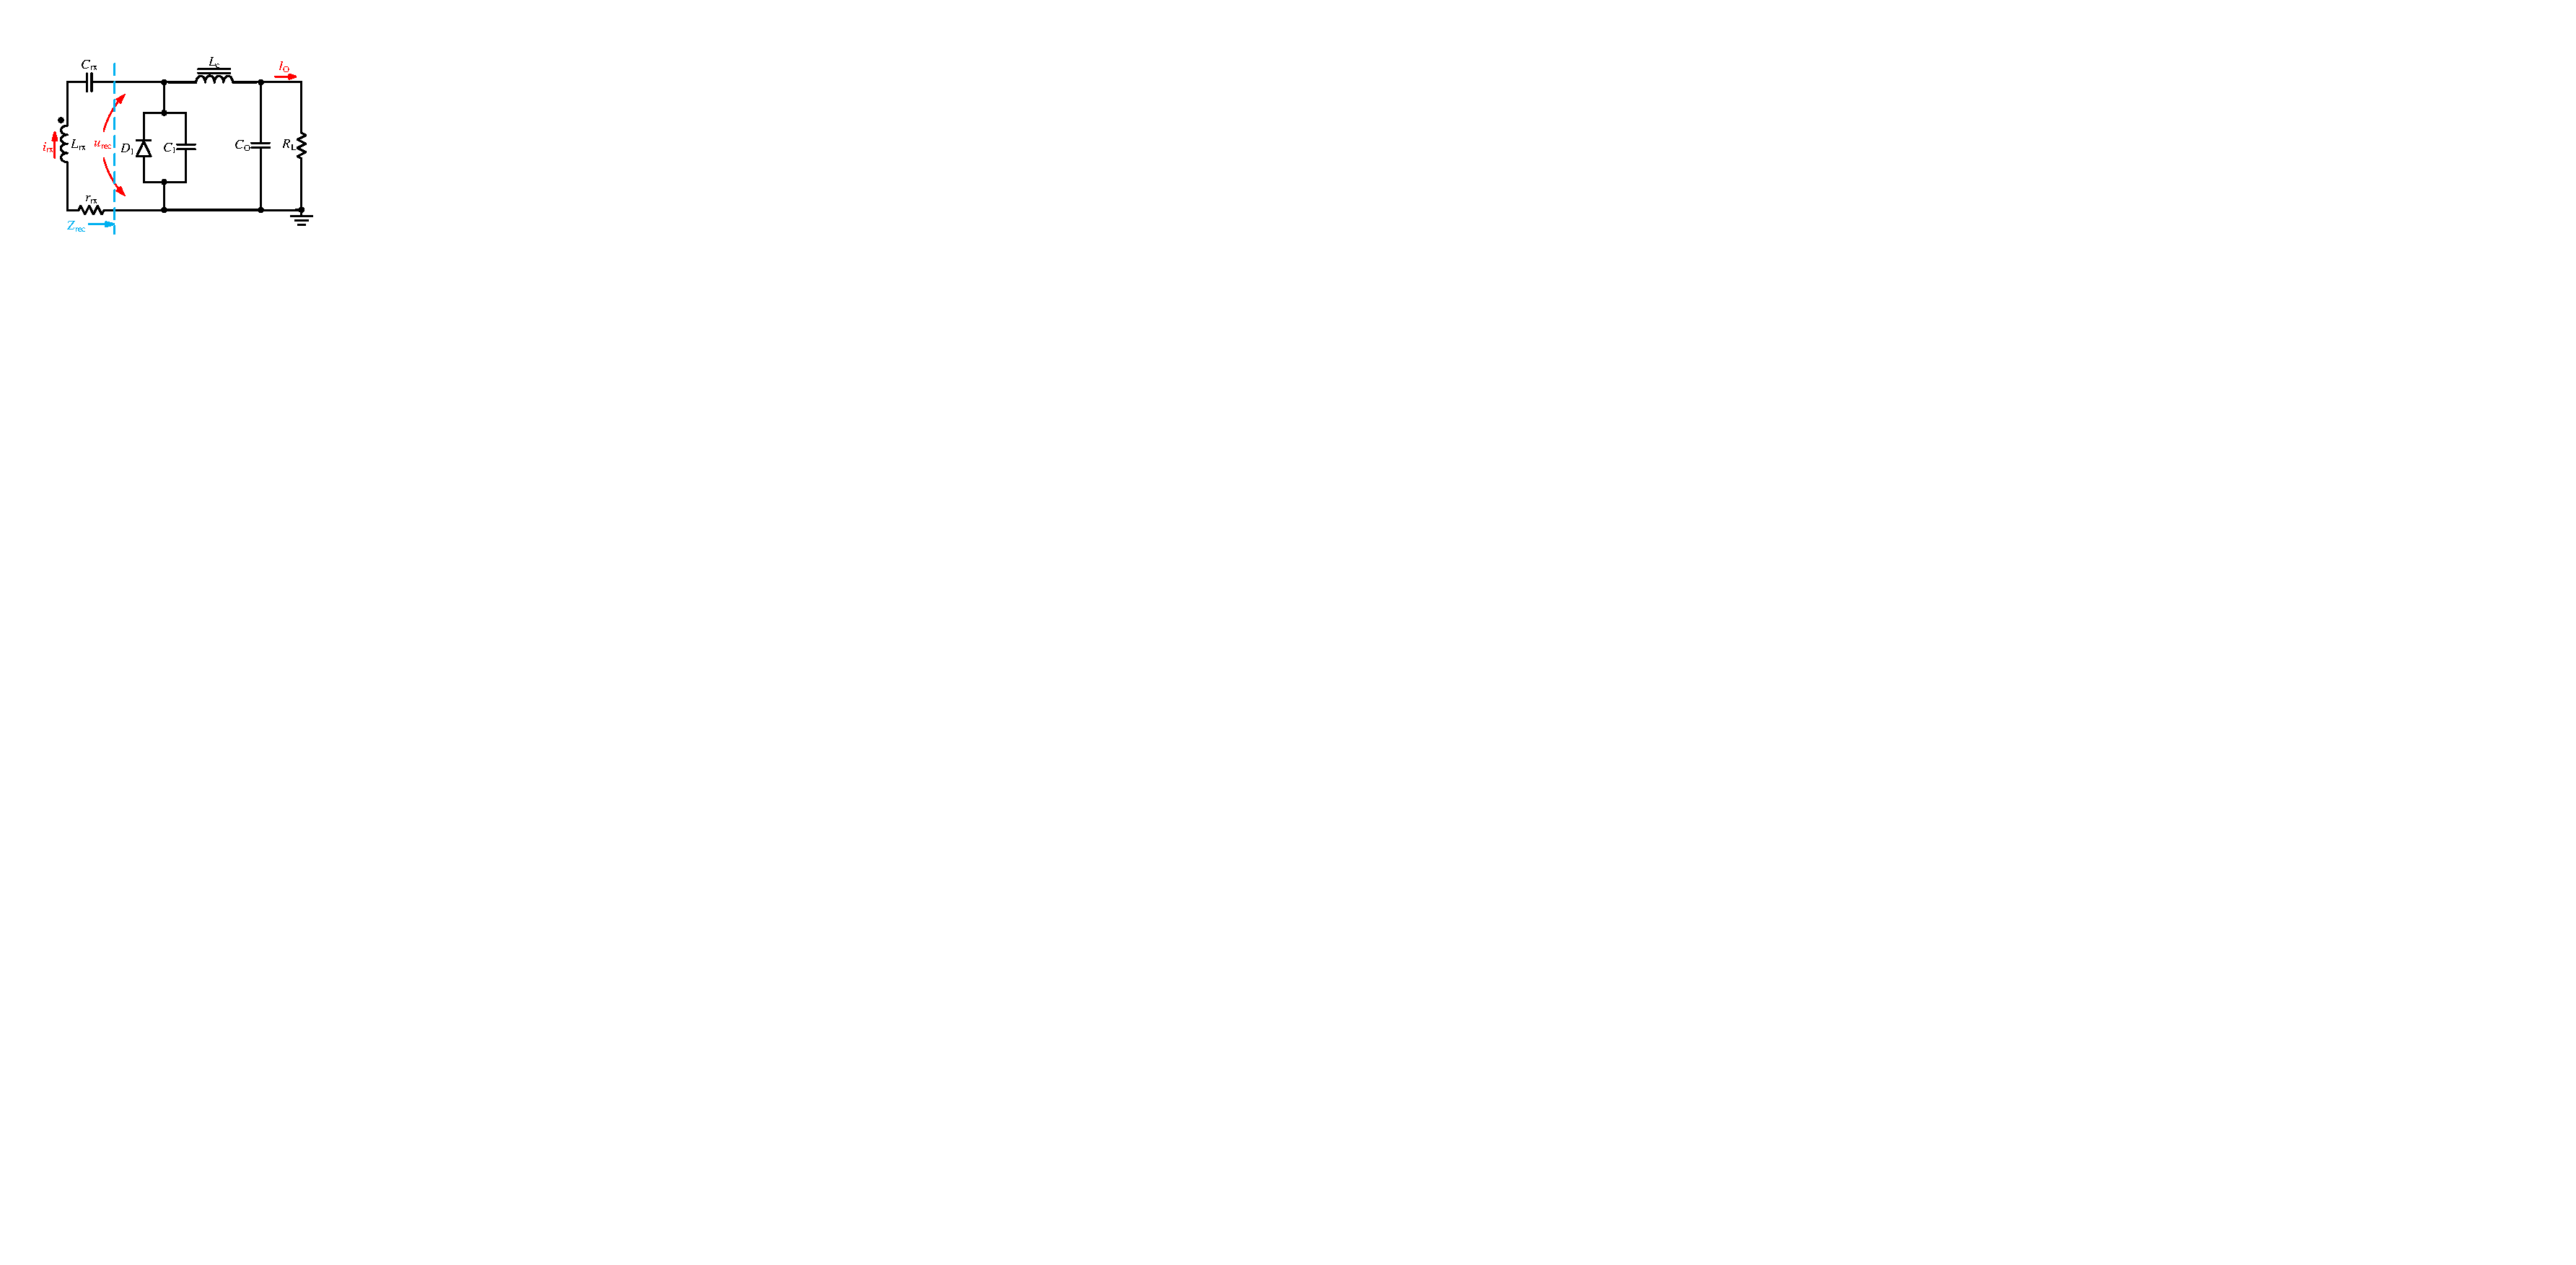
\includegraphics[width=2in]{FiguresEdge/RectifierHalfwave.pdf}}
	\caption{Class E family of rectifiers. (a) Full-wave rectifier. (b) Class EF rectifier. (c) Half-wave rectifier.}
	\label{fig:ClassEfamilyrectifier}
\end{figure}





\ifx\allfiles\undefined
	\onehalfspacing
	\bibliographystyle{chicago}
	%****************************************************************
	%=========This is the file that contains your bibliography entries=======
	%****************************************************************
	\bibliography{HuanBib}
	%=======================================================
	\end{document}
\fi=======================================

%\cleardoublepage
%%\ifx\allfiles\undefined
	\include{Config} %deifne the using package and the paper layout
	\begin{document}
\else
	
\fi
\chapter{Chapter3 Name}
\section{Overview}
Here is the overview of chapter3. Here is the overview of chapter3. Here is the overview of chapter3. Here is the overview of chapter3.

Here is the overview of chapter3. Here is the overview of chapter3. Here is the overview of chapter3. Here is the overview of chapter3.

Here is the overview of chapter3. Here is the overview of chapter3. Here is the overview of chapter3. Here is the overview of chapter3.

Here is the overview of chapter3. Here is the overview of chapter3. Here is the overview of chapter3. Here is the overview of chapter3.

Here is the overview of chapter3. Here is the overview of chapter3. Here is the overview of chapter3. Here is the overview of chapter3.

Here is the overview of chapter3. Here is the overview of chapter3. Here is the overview of chapter3. Here is the overview of chapter3.


\section{Section3}
\label{sec:ModularMRSystem}

\subsection{Modular Architecture}
ABCDE

\ifx\allfiles\undefined
	\onehalfspacing
	\bibliographystyle{chicago}
	%****************************************************************
	%=========This is the file that contains your bibliography entries=======
	%****************************************************************
	\bibliography{HuanBib}
	%=======================================================
	\end{document}
\fi
%%\cleardoublepage
%%\ifx\allfiles\undefined
	\include{Config}
	\begin{document}
\else
	
\fi
\chapter{Current Status and Working Plan}
\section{Overview}
Here is the overview. Here is the overview Here is the overview. Here is the overview. Here is the overview.

Here is the overview. Here is the overview Here is the overview. Here is the overview. Here is the overview

Here is the overview. Here is the overview Here is the overview. Here is the overview. Here is the overview

Here is the overview. Here is the overview Here is the overview. Here is the overview. Here is the overview

Here is the overview. Here is the overview Here is the overview. Here is the overview. Here is the overview

Here is the overview. Here is the overview Here is the overview. Here is the overview. Here is the overview
\section{Summary}\label{sec:Chapter4summary}
Here is the Summary.

\ifx\allfiles\undefined
	\onehalfspacing
	\bibliographystyle{chicago}
	%****************************************************************
	%=========This is the file that contains your bibliography entries=======
	%****************************************************************
	\bibliography{HuanBib}
	%=======================================================
	\end{document}
\fi



%%\cleardoublepage
%%\include{Chapter5}
%%\cleardoublepage
%\include{Conclusion}
%\cleardoublepage
%\chapter*{ACKNOWLEDGEMENT}

Here I would like to thank all the individuals who provide your kind supports and assistances to me and finally make this dissertation possible. It is hard to use words to express my gratitude to all of you.

Foremost, I want to express my heartfelt thanks to my Ph.D supervisor Prof.Chengbin Ma. His wisdom, knowledge, and encouragement really make me to mature as a qualified researcher.
Without his guidance, it is hard for me to make all the accomplishments what I have already achieved. 

Moreover, I would like to express my gratitude to my dissertation committee members, Prof. Houjun Tang, Prof. Jigang Wu, Prof. Mian Li, and Prof. Xinen Zhu. Their detailed guidance and insightful comments are very helpful to further improve the quality of this dissertation and make it more solid, both in terms of technical contents and readability. Also, many thanks to Prof. Patrick Chi-Kwong LUK and Dr. Songnan Yang for their worthful guidance and advice on my research works, especially at the very beginning of my research.

And then, I am grateful to all my lab mates for their selfless helps. I am very enjoy the time working with them all. I also thank the JI staffs for your kind supports throughout my Ph.D program.

Finally, I want to give the special thanks to my family, especially my wife and my son. I will never forget the debt I owe you for your gratuitous support and understanding in the past three years. For this sake, I dedicate the dissertation to you.





%\cleardoublepage
%\include{Appendix}
%\cleardoublepage
%\onehalfspacing
%\bibliographystyle{chicago}
%%****************************************************************
%%=========This is the file that contains your bibliography entries=======
%%****************************************************************
%\bibliography{References}
%%=======================================================
%\end{document}

	\begin{document}
\else
	
\fi
\chapter{Current Status and Working Plan}
\section{Overview}
Here is the overview. Here is the overview Here is the overview. Here is the overview. Here is the overview.

Here is the overview. Here is the overview Here is the overview. Here is the overview. Here is the overview

Here is the overview. Here is the overview Here is the overview. Here is the overview. Here is the overview

Here is the overview. Here is the overview Here is the overview. Here is the overview. Here is the overview

Here is the overview. Here is the overview Here is the overview. Here is the overview. Here is the overview

Here is the overview. Here is the overview Here is the overview. Here is the overview. Here is the overview
\section{Summary}\label{sec:Chapter4summary}
Here is the Summary.

\ifx\allfiles\undefined
	\onehalfspacing
	\bibliographystyle{chicago}
	%****************************************************************
	%=========This is the file that contains your bibliography entries=======
	%****************************************************************
	\bibliography{HuanBib}
	%=======================================================
	\end{document}
\fi



%%\cleardoublepage
%%\include{Chapter5}
%%\cleardoublepage
%\include{Conclusion}
%\cleardoublepage
%\chapter*{ACKNOWLEDGEMENT}

Here I would like to thank all the individuals who provide your kind supports and assistances to me and finally make this dissertation possible. It is hard to use words to express my gratitude to all of you.

Foremost, I want to express my heartfelt thanks to my Ph.D supervisor Prof.Chengbin Ma. His wisdom, knowledge, and encouragement really make me to mature as a qualified researcher.
Without his guidance, it is hard for me to make all the accomplishments what I have already achieved. 

Moreover, I would like to express my gratitude to my dissertation committee members, Prof. Houjun Tang, Prof. Jigang Wu, Prof. Mian Li, and Prof. Xinen Zhu. Their detailed guidance and insightful comments are very helpful to further improve the quality of this dissertation and make it more solid, both in terms of technical contents and readability. Also, many thanks to Prof. Patrick Chi-Kwong LUK and Dr. Songnan Yang for their worthful guidance and advice on my research works, especially at the very beginning of my research.

And then, I am grateful to all my lab mates for their selfless helps. I am very enjoy the time working with them all. I also thank the JI staffs for your kind supports throughout my Ph.D program.

Finally, I want to give the special thanks to my family, especially my wife and my son. I will never forget the debt I owe you for your gratuitous support and understanding in the past three years. For this sake, I dedicate the dissertation to you.





%\cleardoublepage
%\include{Appendix}
%\cleardoublepage
%\onehalfspacing
%\bibliographystyle{chicago}
%%****************************************************************
%%=========This is the file that contains your bibliography entries=======
%%****************************************************************
%\bibliography{References}
%%=======================================================
%\end{document}
